%=============================================================
%  DSA HANDBOOK — Java Edition
%  Fundamentals → ArrayList
%  Compiled with XeLaTeX
%=============================================================
\documentclass[12pt,a4paper,oneside]{book}

%--- geometry ---
\usepackage[a4paper, margin=0.8in]{geometry}

%--- XeLaTeX fonts ---
\usepackage{fontspec}
\usepackage{unicode-math}
\setmainfont{TeX Gyre Pagella}
\setmonofont[Scale=0.88]{TeX Gyre Cursor}
\setmathfont{Latin Modern Math}

%--- spacing ---
\setlength{\parindent}{0pt}
\setlength{\parskip}{6pt}

%--- core packages ---
\usepackage{microtype}
\usepackage{xcolor}
\usepackage{listings}
\usepackage{tcolorbox}
\tcbuselibrary{skins,breakable}
\usepackage{fancyhdr}
\usepackage{titlesec}
\usepackage{booktabs}
\usepackage{array}
\usepackage{colortbl}
\usepackage{longtable}
\usepackage{amsmath}
% Global table spacing
\renewcommand{\arraystretch}{1.35}
\setlength{\tabcolsep}{7pt}

\usepackage{tikz}
\usetikzlibrary{shapes,arrows.meta,positioning,fit,calc,
                decorations.pathreplacing,shapes.geometric,
                shapes.misc}
\usepackage{mdframed}
\usepackage{enumitem}
\usepackage{emptypage}

%=============================================================
%  COLOUR PALETTE — defined early so tocloft/hyperref can use them
%=============================================================
\definecolor{myblue}{RGB}{20,60,120}
\definecolor{mybluelt}{RGB}{25,84,155}
\definecolor{myorange}{RGB}{210,100,0}
\definecolor{mygreen}{RGB}{30,130,60}
\definecolor{myred}{RGB}{190,35,35}
\definecolor{myredlt}{RGB}{200,50,50}
\definecolor{myteal}{RGB}{0,110,100}
\definecolor{mysteelblue}{RGB}{50,90,140}
\definecolor{mygray}{RGB}{90,90,100}
\definecolor{coverbg}{RGB}{18,28,52}

% tint bases
\colorlet{myblue!10}{myblue!10}
\colorlet{myorange!10}{myorange!10}
\colorlet{mygreen!10}{mygreen!10}
\colorlet{myred!10}{myred!10}

% box backgrounds
\definecolor{defbg}{RGB}{238,244,255}
\definecolor{dryrunbg}{RGB}{255,250,235}
\definecolor{tipbg}{RGB}{236,252,242}
\definecolor{warnbg}{RGB}{255,246,230}
\definecolor{cpxbg}{RGB}{237,241,255}
\definecolor{intbg}{RGB}{255,238,238}
\definecolor{codebg}{RGB}{246,248,250}
\definecolor{codeborder}{RGB}{208,215,222}
\definecolor{codecomment}{RGB}{106,153,85}
\definecolor{codekeyword}{RGB}{0,92,197}
\definecolor{codestring}{RGB}{3,119,59}
\definecolor{codenumber}{RGB}{160,80,10}

%--- tocloft: TOC styling (colors now available) ---
\usepackage{tocloft}
% "Contents" heading: Red only — entries follow blue/teal/steelblue hierarchy
\renewcommand{\cfttoctitlefont}{\huge\bfseries\color{myred}}
\renewcommand{\cftaftertoctitle}{\par\noindent\color{black}\rule{\linewidth}{1.5pt}\vspace{2pt}\par\noindent\color{black!20}\rule{\linewidth}{0.5pt}}
\setlength{\cftbeforetoctitleskip}{0pt}
\setlength{\cftaftertoctitleskip}{16pt}
% TOC entries: chapter=blue bold, section=teal, subsection=steelblue small
\renewcommand{\cftchapfont}{\bfseries\color{myblue}}
\renewcommand{\cftchappagefont}{\bfseries\color{myblue}}
\renewcommand{\cftsecfont}{\color{myteal}}
\renewcommand{\cftsecpagefont}{\color{myteal}}
\renewcommand{\cftsubsecfont}{\small\color{mysteelblue}}
\renewcommand{\cftsubsecpagefont}{\small\color{mysteelblue}}

%--- hyperref last (after colors and tocloft) ---
\usepackage[bookmarks=true,
            colorlinks=true,
            linkcolor=black,
            urlcolor=mybluelt,
            pdftitle={DSA Handbook — Java Edition},
            pdfauthor={Biraj}]{hyperref}
% Override hyperref chapter/section link colors to match our hierarchy
\AtBeginDocument{
  \hypersetup{linkcolor=black}
}

%=============================================================
%  LISTINGS — GitHub Light style (NEVER dark background)
%=============================================================
\lstdefinestyle{JavaStyle}{
  language=Java,
  backgroundcolor=\color{codebg},
  basicstyle=\ttfamily\small\color{black},
  keywordstyle=\bfseries\color{codekeyword},
  stringstyle=\color{codestring},
  commentstyle=\itshape\color{codecomment},
  numberstyle=\tiny\color{mygray},
  numbers=left,
  numbersep=10pt,
  stepnumber=1,
  breaklines=true,
  tabsize=4,
  showspaces=false,
  showstringspaces=false,
  frame=single,
  framesep=6pt,
  rulecolor=\color{codeborder},
  xleftmargin=20pt,
  xrightmargin=4pt,
  captionpos=b,
  morekeywords={String,System,out,println,print,printf,length,
                Arrays,Math,ArrayList,HashMap,Scanner,Integer,
                Collections,containsKey,get,put,add,size,
                isEmpty,nextInt,nextLine,nextDouble,close,
                MIN_VALUE,MAX_VALUE,abs,max,min,reverse}
}
\lstset{style=JavaStyle}

%=============================================================
%  TCOLORBOX ENVIRONMENTS
%=============================================================
\tcbset{
  mydefstyle/.style={
    enhanced, breakable, arc=5pt,
    colback=defbg, colframe=myblue,
    fonttitle=\bfseries\color{white}, coltitle=white,
    attach boxed title to top left={yshift=-2mm, xshift=8mm},
    boxed title style={colback=myblue, arc=3pt},
    left=9pt, right=9pt, top=14pt, bottom=10pt,
    parskip=7pt},
  mywarnstyle/.style={
    enhanced, arc=4pt,
    colback=warnbg, colframe=myorange,
    fonttitle=\bfseries, left=9pt, right=9pt,
    top=8pt, bottom=8pt,
    parskip=7pt},
  mytipstyle/.style={
    enhanced, arc=4pt,
    colback=tipbg, colframe=mygreen,
    fonttitle=\bfseries, left=9pt, right=9pt,
    top=8pt, bottom=8pt,
    parskip=7pt},
  mydrstyle/.style={
    enhanced, breakable, arc=5pt,
    colback=dryrunbg, colframe=myorange,
    fonttitle=\bfseries\color{white}, coltitle=white,
    attach boxed title to top left={yshift=-2mm, xshift=8mm},
    boxed title style={colback=myorange, arc=3pt},
    left=9pt, right=9pt, top=14pt, bottom=10pt,
    parskip=7pt},
  mycpxstyle/.style={
    enhanced, arc=4pt,
    colback=cpxbg, colframe=mybluelt,
    fonttitle=\bfseries\color{white}, coltitle=white,
    attach boxed title to top left={yshift=-2mm, xshift=8mm},
    boxed title style={colback=mybluelt, arc=3pt},
    left=9pt, right=9pt, top=14pt, bottom=10pt,
    parskip=7pt},
  myintstyle/.style={
    enhanced, arc=4pt,
    colback=intbg, colframe=myred,
    fonttitle=\bfseries\color{white}, coltitle=white,
    attach boxed title to top left={yshift=-2mm, xshift=8mm},
    boxed title style={colback=myred, arc=3pt},
    left=9pt, right=9pt, top=14pt, bottom=10pt,
    parskip=7pt},
}
\newtcolorbox{definitionbox}[1]{mydefstyle, title={#1}}
\newtcolorbox{warningbox}[1][Note]{mywarnstyle, title={#1}}
\newtcolorbox{tipbox}[1][Tip]{mytipstyle, title={#1}}
\newtcolorbox{dryrun}[1][Dry Run]{mydrstyle, title={#1}}
\newtcolorbox{complexity}[1][Complexity Analysis]{mycpxstyle, title={#1}}
\newtcolorbox{interviewcorner}[1][Interview Corner]{myintstyle, title={#1}}

%=============================================================
%  CHAPTER / SECTION TITLES  —  4-level colour hierarchy
%  Chapter → Deep Red  |  Section  → Deep Blue
%  Subsection → Teal   |  Subsubsection → Steel Blue
%=============================================================
\titleformat{\chapter}[display]
  {\normalfont\huge\bfseries\protect\color{myred}}
  {\filleft\large\protect\color{myorange}\MakeUppercase{Chapter}\ \thechapter}
  {8pt}
  {\protect\color{black}\rule{\linewidth}{1.5pt}\vspace{4pt}\newline\protect\color{myred}}
  [\vspace{2pt}\protect\color{black!25}\rule{\linewidth}{0.5pt}]

\titlespacing*{\chapter}{0pt}{10pt}{16pt}

\titleformat{\section}
  {\normalfont\Large\bfseries\color{myblue}}
  {\thesection}{1em}{}
  [\vspace{-4pt}\color{black!20}\rule{\linewidth}{0.5pt}]
\titlespacing*{\section}{0pt}{18pt}{8pt}

\titleformat{\subsection}
  {\normalfont\large\bfseries\color{myteal}}
  {\thesubsection}{1em}{}
\titlespacing*{\subsection}{0pt}{14pt}{6pt}

\titleformat{\subsubsection}
  {\normalfont\normalsize\bfseries\color{mysteelblue}}
  {\thesubsubsection}{1em}{}
\titlespacing*{\subsubsection}{0pt}{10pt}{4pt}

%=============================================================
%  HEADER / FOOTER
%=============================================================
\pagestyle{fancy}
\fancyhf{}
\fancyhead[L]{\small\color{mygray}\textit{DSA Handbook --- Java Edition}}
\fancyhead[R]{\small\color{mygray}\textit{\nouppercase{\leftmark}}}
\fancyfoot[L]{\small\color{mygray!60}\textit{© Biraj's Notes}}
\fancyfoot[R]{\small\color{mygray}\thepage}
\renewcommand{\headrulewidth}{0.4pt}
\renewcommand{\footrulewidth}{0.2pt}

%--- list spacing ---
\setlist[itemize]{noitemsep, topsep=3pt, leftmargin=1.4em}
\setlist[enumerate]{noitemsep, topsep=3pt, leftmargin=1.6em}

%--- uniform vertical gap around every tcolorbox ---
\tcbset{
  before skip=14pt,
  after skip=14pt,
}

%=============================================================
\begin{document}
%=============================================================

%-------------------------------------------------------------
%  COVER PAGE — white theme, professional branding
%-------------------------------------------------------------
\begin{titlepage}
\pagecolor{white}
\color{black}

% Full-page layout using TikZ for pixel-perfect placement
\begin{tikzpicture}[remember picture, overlay]

  % ── Left red sidebar stripe ──────────────────────────────
  \fill[myred] (current page.north west)
    rectangle ([xshift=1.1cm]current page.south west);

  % ── Top bar (thin, full width) ───────────────────────────
  \fill[myred] (current page.north west)
    rectangle ([yshift=-0.55cm]current page.north east);

  % ── Bottom bar ───────────────────────────────────────────
  \fill[myred!20] (current page.south west)
    rectangle ([yshift=0.45cm]current page.south east);

  % ── Decorative large faint "DSA" watermark behind title ──
  \node[anchor=west, opacity=0.04, font=\fontsize{180}{180}\selectfont\bfseries]
    at ([xshift=1.4cm, yshift=1.5cm]current page.west) {DSA};

\end{tikzpicture}

% ── Main content block ───────────────────────────────────────
\noindent\hspace{1.6cm}%
\begin{minipage}{0.82\textwidth}
\vspace*{1.2cm}

  % Category tag
  {\small\bfseries\color{myred}\MakeUppercase{Personal Study Handbook}
   \hspace{6pt}\textcolor{black!25}{\rule[0.6ex]{1.8cm}{0.4pt}}\hspace{6pt}
   \textcolor{black!55}{\textit{Java Edition}}}

  \vspace{0.55cm}

  % Main title
  {\fontsize{62}{66}\selectfont\bfseries\color{black}DSA}\\[0pt]
  {\fontsize{28}{32}\selectfont\bfseries\color{black}Handbook}

  \vspace{0.42cm}

  % Bold red rule
  {\color{myred}\rule{9.5cm}{3pt}}

  \vspace{0.55cm}

  % Subtitle — full black, not grey
  {\large\bfseries\color{black!85} From Fundamentals to 2-D Arrays}

  \vspace{0.3cm}

  % Tag pills — stronger color
  \foreach \tag in {Beginner-Friendly, Interview-Oriented, Deeply Explained}{%
    \tikz[baseline=-0.5ex]\node[%
      fill=myred!12, draw=myred!50, rounded corners=10pt,
      inner xsep=9pt, inner ysep=4pt,
      font=\small\bfseries\color{myred}]{\tag};\hspace{5pt}%
  }

  \vspace{1.3cm}

  % ── Array visualisation ──────────────────────────────────
  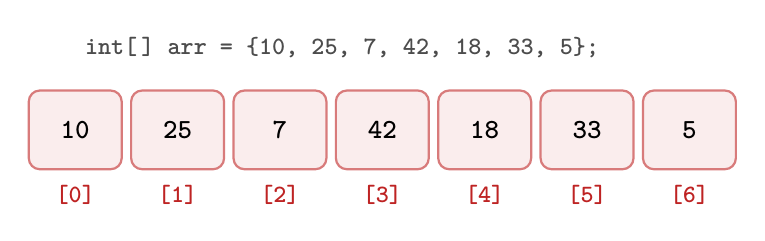
\begin{tikzpicture}
    \node[font=\small\ttfamily\bfseries\color{black!70}, anchor=west]
      at (0, 1.05) {int[\,] arr\ =\ \{10,\ 25,\ 7,\ 42,\ 18,\ 33,\ 5\};};
    \foreach \v/\i in {10/0, 25/1, 7/2, 42/3, 18/4, 33/5, 5/6}{
      \node[draw=myred!60, fill=myred!8, line width=0.8pt,
            minimum width=1.18cm, minimum height=1.0cm,
            rounded corners=4pt,
            font=\ttfamily\normalsize\bfseries\color{black}]
        at (\i*1.30, 0) {\v};
      \node[font=\small\ttfamily\bfseries\color{myred}]
        at (\i*1.30,-0.82) {[\i]};
    }
  \end{tikzpicture}

  \vspace{1.5cm}

  % Separator
  {\color{black!20}\rule{9.5cm}{0.6pt}}

  \vspace{0.45cm}

  % References — darker, readable
  {\normalsize\color{black!70}
    Based on \textbf{\color{black}TakeUForward} (Striver),
    \textbf{\color{black}Love Babbar} \&
    \textbf{\color{black}APNA CLG DSA} Series
  }

  \vspace{0.25cm}

  {\small\color{black!50}
    \textbullet\ w3schools.com\quad
    \textbullet\ geeksforgeeks.org\quad
    \textbullet\ codehelp.in\quad
    \textbullet\ apnacollege.in
  }

  \vspace{2.0cm}

  % ── Author block ─────────────────────────────────────────
  \begin{minipage}{0.52\textwidth}
    {\LARGE\bfseries\color{black} Biraj}\\[4pt]
    {\normalsize\color{black!70} ECE Student \ $\cdot$\ Full-Stack Developer}\\[4pt]
    {\normalsize\bfseries\color{myred} github.com/Biraj2004}
  \end{minipage}%
  \hfill
  \begin{minipage}{0.40\textwidth}\raggedleft
    {\normalsize\bfseries\color{black} Version 1.0}\\[4pt]
    {\normalsize\color{black!65} May 2026}
  \end{minipage}

  \vspace{0.6cm}

\end{minipage}

\end{titlepage}
\nopagecolor

%=============================================================
\frontmatter
%=============================================================
\tableofcontents
\clearpage

%=============================================================
%  HOW TO USE THIS HANDBOOK
%=============================================================
\chapter*{How to Use This Handbook}
\addcontentsline{toc}{chapter}{How to Use This Handbook}
\markboth{How to Use This Handbook}{}

This handbook is your structured companion for learning Data Structures \& Algorithms in Java --- from the very first concept to mastering 2-D Arrays. It is written to be \textbf{shallow-to-medium depth}: clear enough to understand quickly, deep enough to perform in interviews.

\begin{definitionbox}{Structure of Each Topic}
\begin{enumerate}
  \item \textbf{Concept} --- What it is, in plain English
  \item \textbf{Java Code} --- Clean implementation (no step-jumps; every line explained)
  \item \textbf{Dry Run} --- Step-by-step table trace on a small example
  \item \textbf{Visual Diagram} --- Memory or execution diagram where helpful
  \item \textbf{Complexity} --- Time and Space Big-O analysis
  \item \textbf{Interview Corner} --- What interviewers ask, edge cases, tricks
\end{enumerate}
\end{definitionbox}

\begin{warningbox}[Box Colour Guide]
\textbf{Blue box} --- Core definition / concept\\
\textbf{Orange box (Dry Run)} --- Step-by-step trace table\\
\textbf{Indigo box (Complexity)} --- Big-O analysis\\
\textbf{Red box (Interview Corner)} --- Interview questions \& edge cases\\
\textbf{Green box (Tip)} --- Shortcuts, tricks, common mistakes
\end{warningbox}

%=============================================================
\mainmatter
%=============================================================

%%############################################################
\chapter{Fundamentals of Programming}
%%############################################################

\section{What is a Program?}

A \textbf{program} is a set of instructions given to a computer to solve a problem. You write those instructions in a \textbf{programming language} (like Java), and the computer executes them one by one.

\begin{definitionbox}{Essential Terms}
\begin{itemize}
  \item \textbf{Source Code} --- The human-readable instructions you type
  \item \textbf{Compiler} --- Translates source code into machine-understandable code
  \item \textbf{JVM (Java Virtual Machine)} --- Runs compiled Java bytecode on any operating system
  \item \textbf{Algorithm} --- A finite, step-by-step procedure that solves a problem
  \item \textbf{Data Structure} --- A way to organise, store, and access data efficiently
\end{itemize}
\end{definitionbox}

\section{How Java Works}

Java follows a two-step process: compile once, run anywhere.

\begin{center}
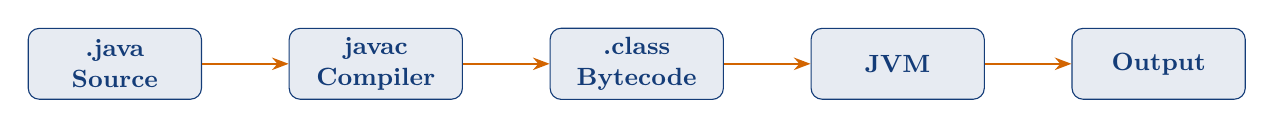
\begin{tikzpicture}[
  box/.style={
    rectangle, draw=myblue, fill=myblue!10,
    rounded corners=4pt,
    minimum width=2.2cm, minimum height=0.9cm,
    font=\small\bfseries, text=myblue, align=center},
  arr/.style={-{Stealth[length=6pt]}, thick, color=myorange}
]
  \node[box](src){.java\\Source};
  \node[box, right=1.1cm of src](javac){javac\\Compiler};
  \node[box, right=1.1cm of javac](cls){.class\\Bytecode};
  \node[box, right=1.1cm of cls](jvm){JVM};
  \node[box, right=1.1cm of jvm](out){Output};
  \draw[arr](src)--(javac);
  \draw[arr](javac)--(cls);
  \draw[arr](cls)--(jvm);
  \draw[arr](jvm)--(out);
\end{tikzpicture}
\end{center}

\begin{enumerate}
  \item You write code in a \texttt{.java} file
  \item \texttt{javac} compiles it to a \texttt{.class} file (bytecode)
  \item The JVM reads bytecode and executes it on your machine
  \item The result appears as output (console, file, etc.)
\end{enumerate}

\textbf{Key advantage of JVM:} The same \texttt{.class} file runs on Windows, Linux, or macOS without recompilation --- ``Write Once, Run Anywhere.''

\section{Your First Java Program}

\begin{lstlisting}[caption={Hello World in Java --- Every line explained}]
// A comment: ignored by compiler, just for you to read

public class HelloWorld {     // every Java file needs a class
                              // class name MUST match filename

    // main() is the entry point - JVM starts here
    public static void main(String[] args) {

        // println prints text then moves to the next line
        System.out.println("Hello, World!");

    }  // end of main
}      // end of class
\end{lstlisting}

\begin{dryrun}[Dry Run: Hello World]
\begin{enumerate}
  \item JVM locates \texttt{main()} and enters it
  \item Executes \texttt{System.out.println("Hello, World!")} --- sends text to console
  \item Prints: \texttt{Hello, World!}
  \item \texttt{main()} reaches its closing brace \texttt{\}} and exits
  \item Program terminates
\end{enumerate}
\end{dryrun}

\section{Flowcharts and Pseudocode}

Before writing code, professionals plan their logic using flowcharts or pseudocode. This catches errors early and makes coding faster.

\subsection{Flowchart Symbols}

\begin{center}
\begin{tabular}{lll}
\toprule
\textbf{Shape} & \textbf{Name} & \textbf{Represents}\\
\midrule
Oval (rounded box)  & Terminator    & Start or End of program\\
Rectangle           & Process       & A computation or action\\
Diamond             & Decision      & A yes/no branch (if/else)\\
Parallelogram       & Input/Output  & Reading input or printing output\\
Arrow               & Flow line     & Direction of execution\\
\bottomrule
\end{tabular}
\end{center}

\subsection{Flowchart: Is a Number Even or Odd?}

\begin{center}
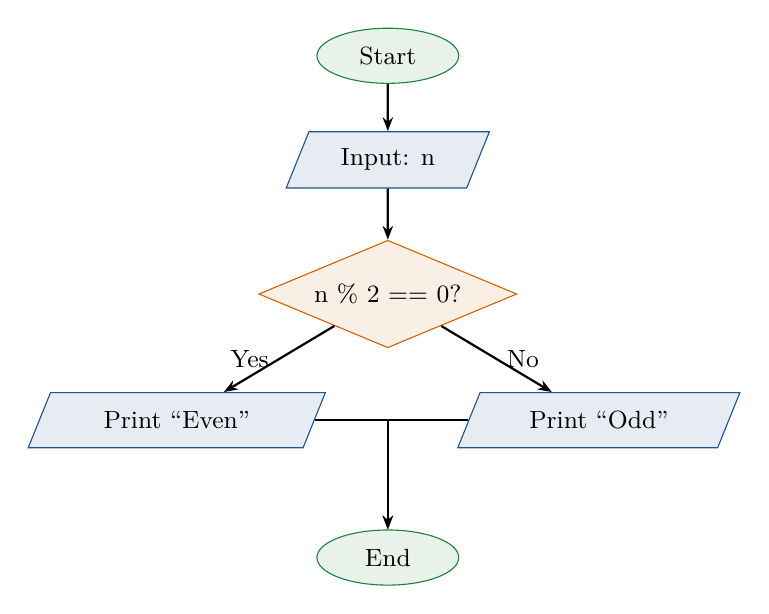
\begin{tikzpicture}[
  term/.style={ellipse, draw=mygreen, fill=mygreen!10,
               minimum width=1.8cm, minimum height=0.7cm, font=\small},
  io/.style={trapezium, trapezium left angle=68, trapezium right angle=112,
             draw=mybluelt, fill=myblue!10,
             minimum width=2.6cm, minimum height=0.7cm, font=\small},
  dec/.style={diamond, draw=myorange, fill=myorange!10,
              minimum width=2.2cm, minimum height=0.7cm,
              font=\small, aspect=2.4},
  arr/.style={-{Stealth[length=5pt]}, thick}
]
  \node[term](start){Start};
  \node[io, below=0.6cm of start](inp){Input: n};
  \node[dec, below=0.65cm of inp](dec){n \% 2 == 0?};
  \node[io, below left=0.9cm and 1.5cm of dec](even){Print ``Even''};
  \node[io, below right=0.9cm and 1.5cm of dec](odd){Print ``Odd''};
  \node[term, below=2.3cm of dec](end){End};

  \draw[arr](start)--(inp);
  \draw[arr](inp)--(dec);
  \draw[arr](dec)--node[left,font=\small]{Yes}(even);
  \draw[arr](dec)--node[right,font=\small]{No}(odd);
  \draw[arr](even)-|(end);
  \draw[arr](odd)-|(end);
\end{tikzpicture}
\end{center}

\subsection{Pseudocode for Even / Odd}

\begin{mdframed}[linecolor=myblue, linewidth=1pt, backgroundcolor=myblue!10,
                 innerleftmargin=10pt, innerrightmargin=10pt,
                 innertopmargin=8pt, innerbottommargin=8pt]
\begin{verbatim}
BEGIN
  INPUT n
  IF n % 2 == 0 THEN
    PRINT "Even"
  ELSE
    PRINT "Odd"
  END IF
END
\end{verbatim}
\end{mdframed}

%%############################################################
\chapter{Java Language Basics}
%%############################################################

\section{Variables and Data Types}

A \textbf{variable} is a named slot in memory. You give it a name, declare its type, and assign a value.

\begin{center}
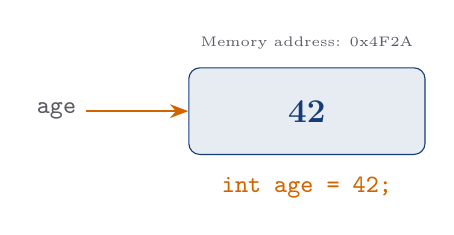
\begin{tikzpicture}[font=\small]
  \node[draw=myblue, fill=myblue!10, minimum width=3cm, minimum height=1.1cm,
        rounded corners=4pt, font=\large\bfseries, text=myblue](box) at (0,0){42};
  \node[below=0.15cm of box, text=myorange, font=\ttfamily\small]
    {\texttt{int age = 42;}};
  \node[above=0.1cm of box, text=mygray, font=\tiny]
    {Memory address: 0x4F2A};
  \draw[myorange, -{Stealth}, thick](-2.8,0)
    node[left, text=mygray, font=\ttfamily\small]{\texttt{age}} -- (box.west);
\end{tikzpicture}
\end{center}

\subsection{Java's Eight Primitive Types}

\begin{center}
{\setlength{\arrayrulewidth}{0.4pt}%
\renewcommand{\arraystretch}{1.4}%
\begin{tabular}{!{\color{black!30}\vrule}l!{\color{black!30}\vrule}l!{\color{black!30}\vrule}l!{\color{black!30}\vrule}l!{\color{black!30}\vrule}l!{\color{black!30}\vrule}}
\toprule
\textbf{Type} & \textbf{Size} & \textbf{Value Range (approx)} & \textbf{Default} & \textbf{Example}\\
\midrule
\texttt{byte}    & 1 byte  & $-128$ to $127$                          & \texttt{0}     & \texttt{byte b = 100;}\\
\texttt{short}   & 2 bytes & $-32{,}768$ to $32{,}767$                & \texttt{0}     & \texttt{short s = 1000;}\\
\texttt{int}     & 4 bytes & $\approx -2.1\text{B}$ to $+2.1\text{B}$& \texttt{0}     & \texttt{int n = 42;}\\
\texttt{long}    & 8 bytes & $\approx \pm 9.2 \times 10^{18}$         & \texttt{0L}    & \texttt{long l = 99L;}\\
\texttt{float}   & 4 bytes & $\approx \pm 3.4 \times 10^{38}$         & \texttt{0.0f}  & \texttt{float f = 3.14f;}\\
\texttt{double}  & 8 bytes & $\approx \pm 1.7 \times 10^{308}$        & \texttt{0.0}   & \texttt{double d = 3.14;}\\
\texttt{char}    & 2 bytes & $0$ to $65{,}535$ (Unicode)               & \texttt{'\textbackslash{}u0000'} & \texttt{char c = 'A';}\\
\texttt{boolean} & 1 bit   & \texttt{true} / \texttt{false}           & \texttt{false} & \texttt{boolean ok = true;}\\
\bottomrule
\end{tabular}}
\end{center}

\begin{lstlisting}[caption={Variables and Data Types in Action}]
public class DataTypesDemo {
    public static void main(String[] args) {

        // Integer family
        int age       = 21;
        long bigNum   = 7_800_000_000L;  // L suffix required for long
        short s       = 500;
        byte b        = 127;             // max value for byte

        // Decimal family
        double pi     = 3.14159265;      // prefer double for accuracy
        float temp    = 36.6f;           // f suffix required for float

        // Character and boolean
        char grade    = 'A';             // single quotes for char
        boolean pass  = true;

        // String -- NOT a primitive; it is a class
        String name   = "Riya";          // double quotes for String

        System.out.println("Name  : " + name);
        System.out.println("Age   : " + age);
        System.out.println("Grade : " + grade);
        System.out.println("PI    : " + pi);
        System.out.println("Pass  : " + pass);
    }
}
\end{lstlisting}

\begin{tipbox}[int vs long vs double]
Use \texttt{int} for whole numbers that fit in 2 billion. Use \texttt{long} for very large counts (populations, timestamps). Use \texttt{double} for decimals in DSA --- it is the most precise floating-point type in Java.
\end{tipbox}

\section{Operators}

\subsection{Arithmetic Operators}

\begin{center}
\begin{tabular}{clll}
\toprule
\textbf{Op} & \textbf{Meaning} & \textbf{Example} & \textbf{Result}\\
\midrule
\texttt{+}  & Addition        & \texttt{10 + 3}  & \texttt{13}\\
\texttt{-}  & Subtraction     & \texttt{10 - 3}  & \texttt{7}\\
\texttt{*}  & Multiplication  & \texttt{10 * 3}  & \texttt{30}\\
\texttt{/}  & Division        & \texttt{10 / 3}  & \texttt{3} (decimal dropped!)\\
\texttt{\%} & Modulus/Remainder & \texttt{10 \% 3} & \texttt{1}\\
\bottomrule
\end{tabular}
\end{center}

\begin{tipbox}[Integer Division Trap]
\texttt{int / int} always drops the decimal part. To get the true decimal result, cast one operand: \texttt{(double) 10 / 3} gives \texttt{3.3333...}
\end{tipbox}

\subsection{Relational and Logical Operators}

\begin{center}
\begin{tabular}{llll}
\toprule
\textbf{Category} & \textbf{Operator} & \textbf{Meaning} & \textbf{Example $\to$ Result}\\
\midrule
Relational & \texttt{==}  & Equal to           & \texttt{5 == 5} $\to$ \texttt{true}\\
           & \texttt{!=}  & Not equal          & \texttt{5 != 3} $\to$ \texttt{true}\\
           & \texttt{>}   & Greater than       & \texttt{7 > 3}  $\to$ \texttt{true}\\
           & \texttt{<}   & Less than          & \texttt{2 < 9}  $\to$ \texttt{true}\\
           & \texttt{>=}  & Greater or equal   & \texttt{5 >= 5} $\to$ \texttt{true}\\
           & \texttt{<=}  & Less or equal      & \texttt{3 <= 4} $\to$ \texttt{true}\\
\midrule
Logical    & \texttt{\&\&}& AND --- both true  & \texttt{T \&\& F} $\to$ \texttt{false}\\
           & \texttt{||}  & OR  --- at least one & \texttt{T || F} $\to$ \texttt{true}\\
           & \texttt{!}   & NOT --- negate     & \texttt{!true}  $\to$ \texttt{false}\\
\bottomrule
\end{tabular}
\end{center}

\section{Input and Output}

\begin{lstlisting}[caption={Reading User Input with Scanner}]
import java.util.Scanner;   // import this class before using it

public class InputDemo {
    public static void main(String[] args) {

        // Create a Scanner connected to the keyboard (System.in)
        Scanner sc = new Scanner(System.in);

        System.out.print("Enter your name: ");
        String name = sc.nextLine();     // reads the whole line

        System.out.print("Enter your age: ");
        int age = sc.nextInt();          // reads one integer

        System.out.print("Enter your GPA: ");
        double gpa = sc.nextDouble();    // reads a decimal number

        // Output
        System.out.println("Name : " + name);
        System.out.println("Age  : " + age);
        System.out.printf("GPA  : %.2f%n", gpa);  // 2 decimal places

        sc.close();   // always close the Scanner
    }
}
\end{lstlisting}

\begin{center}
\begin{tabular}{ll}
\toprule
\textbf{Scanner Method} & \textbf{What it Reads}\\
\midrule
\texttt{sc.nextInt()}      & One integer\\
\texttt{sc.nextLong()}     & One long value\\
\texttt{sc.nextDouble()}   & One decimal (double)\\
\texttt{sc.nextFloat()}    & One decimal (float)\\
\texttt{sc.next()}         & One word (stops at whitespace)\\
\texttt{sc.nextLine()}     & A complete line of text\\
\texttt{sc.nextBoolean()}  & \texttt{true} or \texttt{false}\\
\bottomrule
\end{tabular}
\end{center}

\begin{warningbox}[nextInt() + nextLine() Pitfall]
After \texttt{sc.nextInt()}, the newline character \texttt{`\textbackslash n'} stays in the buffer. If you call \texttt{sc.nextLine()} immediately after, it picks up that leftover newline. Fix: add an extra \texttt{sc.nextLine()} to consume it before reading the string.
\end{warningbox}

\subsection{Output Methods --- print, println, and printf}
\index{Output!print}\index{Output!println}\index{Output!printf}

Java has three ways to print output. Knowing when to use which is essential.

\begin{center}
\renewcommand{\arraystretch}{1.55}
{\small
\begin{tabular}{
  !{\color{myblue}\vrule width 1.2pt}
  >{\bfseries\ttfamily}p{3.9cm}
  !{\color{myblue!40}\vrule}
  p{4.6cm}
  !{\color{myblue!40}\vrule}
  p{3.0cm}
  !{\color{myblue}\vrule width 1.2pt}
}
\arrayrulecolor{myblue}\hline
\rowcolor{myblue}
\color{white}\textbf{Method} &
\color{white}\textbf{What it does} &
\color{white}\textbf{Example output}\\
\arrayrulecolor{myblue}\hline
\rowcolor{myblue!8}
System.out.\newline println() & Prints then moves to \textbf{next line} automatically & \texttt{Hello}\newline(cursor $\to$ next line)\\
\rowcolor{white}
System.out.print() & Prints with \textbf{no newline} --- cursor stays on same line & \texttt{Hello} (cursor stays)\\
\rowcolor{myblue!8}
System.out.printf() & Prints using a \textbf{format string} with placeholders & \texttt{GPA : 8.46}\\
\arrayrulecolor{myblue}\hline
\end{tabular}}
\end{center}

\begin{lstlisting}[caption={print vs println vs printf --- all three compared}]
public class OutputMethods {
    public static void main(String[] args) {

        // println: adds a newline at the end automatically
        System.out.println("Hello");   // prints "Hello" then goes to next line
        System.out.println("World");   // prints "World" on a new line
        // Output:
        // Hello
        // World

        // print: NO newline added; cursor stays on the same line
        System.out.print("Hello ");
        System.out.print("World");
        System.out.println();   // manual newline to end the line
        // Output:
        // Hello World

        // printf: uses a FORMAT STRING with placeholders
        //   %s  --> placeholder for a String
        //   %d  --> placeholder for an integer (int)
        //   %f  --> placeholder for a decimal (double / float)
        //   %.2f --> decimal with exactly 2 digits after the decimal point
        //   %n  --> newline (platform-independent, prefer over \n in printf)

        String name = "Riya";
        int age = 20;
        double gpa = 8.4567;

        System.out.printf("%s is %d years old%n", name, age);
        // Output: Riya is 20 years old

        System.out.printf("GPA : %.2f%n", gpa);
        // Output: GPA : 8.46   (rounded to 2 decimal places)

        // Multiple placeholders: pass values after the format string, in order
        System.out.printf("Name: %s | Age: %d | GPA: %.1f%n", name, age, gpa);
        // Output: Name: Riya | Age: 20 | GPA: 8.5
    }
}
\end{lstlisting}

\begin{definitionbox}{How printf Format Strings Work}
\texttt{printf()} uses a \textbf{format string} first, then the actual values separated by commas.

\begin{center}
\begin{tabular}{ll}
\toprule
\textbf{Placeholder} & \textbf{Meaning}\\
\midrule
\texttt{\%s}   & String\\
\texttt{\%d}   & Integer (\texttt{int}, \texttt{long})\\
\texttt{\%f}   & Floating-point (\texttt{double}, \texttt{float}) --- default 6 decimal places\\
\texttt{\%.2f} & Float with exactly \textbf{2} decimal places (\texttt{.2} controls precision)\\
\texttt{\%n}   & Newline (use instead of \texttt{\textbackslash n} inside \texttt{printf})\\
\texttt{\%b}   & Boolean\\
\bottomrule
\end{tabular}
\end{center}

\vspace{4pt}
\textbf{Example:} \texttt{System.out.printf("GPA : \%.2f\%n", gpa);}

The placeholder \texttt{\%.2f} is \textit{replaced} by the value of \texttt{gpa}, formatted to 2 decimal places.

\texttt{double gpa = 8.4567;} $\xrightarrow{\texttt{printf}}$ \texttt{GPA : 8.46}
\end{definitionbox}

\begin{tipbox}[When to use which?]
\textbf{println} --- most common; use for simple messages, debug output, and when each print goes on its own line.\\[3pt]
\textbf{print} --- use when you want multiple values on the \textit{same line} (e.g., printing array elements separated by spaces).\\[3pt]
\textbf{printf} --- use when you need \textit{formatted} output: fixed decimal places, aligned columns, or embedding variables cleanly inside a string.
\end{tipbox}

\section{Conditional Statements}

\subsection{if / else if / else}

\begin{lstlisting}[caption={Grade Calculator using if-else chain}]
public class GradeCalc {
    public static void main(String[] args) {
        int marks = 75;

        if (marks >= 90) {
            System.out.println("Grade: A");
        } else if (marks >= 75) {
            System.out.println("Grade: B");   // <-- this runs
        } else if (marks >= 60) {
            System.out.println("Grade: C");
        } else if (marks >= 40) {
            System.out.println("Grade: D");
        } else {
            System.out.println("Grade: F");
        }
    }
}
\end{lstlisting}

\begin{dryrun}[Dry Run: marks = 75]
\begin{enumerate}
  \item Check \texttt{75 >= 90}? No $\to$ move to next condition
  \item Check \texttt{75 >= 75}? \textbf{Yes} $\to$ execute this block
  \item Print \texttt{Grade: B}
  \item All remaining \texttt{else if} and \texttt{else} blocks are skipped
\end{enumerate}
\textbf{Output:} \texttt{Grade: B}
\end{dryrun}

\subsection{switch-case}

Use \texttt{switch} when comparing one variable against many fixed values --- it is often cleaner than a long \texttt{else if} chain.

\begin{lstlisting}[caption={Day Name using switch-case}]
public class DayName {
    public static void main(String[] args) {
        int day = 3;

        switch (day) {
            case 1:  System.out.println("Monday");    break;
            case 2:  System.out.println("Tuesday");   break;
            case 3:  System.out.println("Wednesday"); break;  // runs
            case 4:  System.out.println("Thursday");  break;
            case 5:  System.out.println("Friday");    break;
            default: System.out.println("Weekend");
        }
    }
}
\end{lstlisting}

\begin{warningbox}[Always Write break!]
Without \texttt{break}, Java \textit{falls through} into the next case and executes it too. This is one of the most common beginner bugs.
\end{warningbox}

\section{Loops}

\subsection{for Loop}

Use the \texttt{for} loop when you know \textbf{exactly how many times} to repeat.

\begin{lstlisting}[caption={for Loop --- Print 1 to 5}]
public class ForLoopDemo {
    public static void main(String[] args) {

        //   init    condition  update
        for (int i = 1; i <= 5; i++) {
            System.out.println("i = " + i);
        }
    }
}
\end{lstlisting}

\begin{dryrun}[Dry Run: for loop i = 1 to 5]
\begin{center}
\begin{tabular}{cccc}
\toprule
\textbf{Iteration} & \textbf{i} & \textbf{i $\leq$ 5?} & \textbf{Output}\\
\midrule
1 & 1 & true  & \texttt{i = 1}\\
2 & 2 & true  & \texttt{i = 2}\\
3 & 3 & true  & \texttt{i = 3}\\
4 & 4 & true  & \texttt{i = 4}\\
5 & 5 & true  & \texttt{i = 5}\\
6 & 6 & false & Loop ends\\
\bottomrule
\end{tabular}
\end{center}
\end{dryrun}

\subsection{while and do-while Loops}

\begin{lstlisting}[caption={while vs do-while --- key difference shown}]
public class WhileDoWhile {
    public static void main(String[] args) {

        // while: checks condition BEFORE entering the body
        int i = 1;
        while (i <= 5) {
            System.out.print(i + " ");
            i++;              // MUST update -- else infinite loop!
        }
        System.out.println();  // Output: 1 2 3 4 5

        // do-while: runs the body FIRST, then checks condition
        // Body executes at least once even if condition is false
        int j = 10;
        do {
            System.out.println("Ran at least once: j = " + j);
            j++;
        } while (j <= 5);    // false immediately, but body ran once
    }
}
\end{lstlisting}

\subsection{break and continue}

\begin{lstlisting}[caption={break exits the loop; continue skips the current iteration}]
public class BreakContinue {
    public static void main(String[] args) {

        // break: immediately exits the loop
        System.out.print("break at 6: ");
        for (int i = 1; i <= 10; i++) {
            if (i == 6) break;          // stop here
            System.out.print(i + " ");
        }
        // Output: 1 2 3 4 5

        System.out.println();

        // continue: skip the current iteration and move to next
        System.out.print("skip evens: ");
        for (int i = 1; i <= 10; i++) {
            if (i % 2 == 0) continue;  // skip even numbers
            System.out.print(i + " ");
        }
        // Output: 1 3 5 7 9
    }
}
\end{lstlisting}

\begin{tipbox}[Which Loop to Use?]
\textbf{for loop} --- Number of iterations known in advance (most DSA problems).\\
\textbf{while loop} --- Iterate until a condition changes (count unknown).\\
\textbf{do-while} --- Must run at least once (e.g., menu-driven programs).
\end{tipbox}

\section{Methods in Java}

A \textbf{method} is a reusable block of code with a name. It avoids repeating the same code.

\begin{lstlisting}[caption={Defining and calling methods}]
public class MethodsDemo {

    // Method definition: returnType methodName(parameters)
    public static int add(int a, int b) {
        int result = a + b;
        return result;   // sends value back to caller
    }

    // void means no return value
    public static void greet(String name) {
        System.out.println("Hello, " + name + "!");
    }

    public static void main(String[] args) {
        int sum = add(10, 20);       // call the method
        System.out.println("Sum = " + sum);   // Sum = 30

        greet("Priya");    // Hello, Priya!
        greet("Arjun");    // Hello, Arjun!
    }
}
\end{lstlisting}

%%############################################################
\chapter{Time and Space Complexity}
%%############################################################

\section{Why Complexity Matters}

Two programs that produce the same correct output can behave very differently when the input is large. Understanding complexity tells you \textit{before coding} whether your approach will be fast enough.

\begin{definitionbox}{Big-O Notation}
Big-O describes the \textbf{worst-case growth rate} of an algorithm as input size $n \to \infty$. It ignores constant factors and smaller terms.

$$T(n) = 5n^2 + 3n + 100 \implies O(n^2)$$

Think of it as: \textit{``As n grows very large, how does the running time grow?''}
\end{definitionbox}

\section{Common Complexity Classes}

\begin{center}
\begin{tabular}{lllr}
\toprule
\textbf{Notation} & \textbf{Name} & \textbf{Classic Example} & \textbf{n = 1000 (ops)}\\
\midrule
$O(1)$        & Constant     & Array index access    & 1\\
$O(\log n)$   & Logarithmic  & Binary Search         & $\approx 10$\\
$O(n)$        & Linear       & Linear Search         & 1,000\\
$O(n \log n)$ & Linearithmic & Merge Sort            & $\approx 10{,}000$\\
$O(n^2)$      & Quadratic    & Bubble Sort           & 1,000,000\\
$O(n^3)$      & Cubic        & Triple-nested loop    & $10^9$\\
$O(2^n)$      & Exponential  & All subsets           & $\approx 10^{301}$\\
\bottomrule
\end{tabular}
\end{center}

\begin{center}
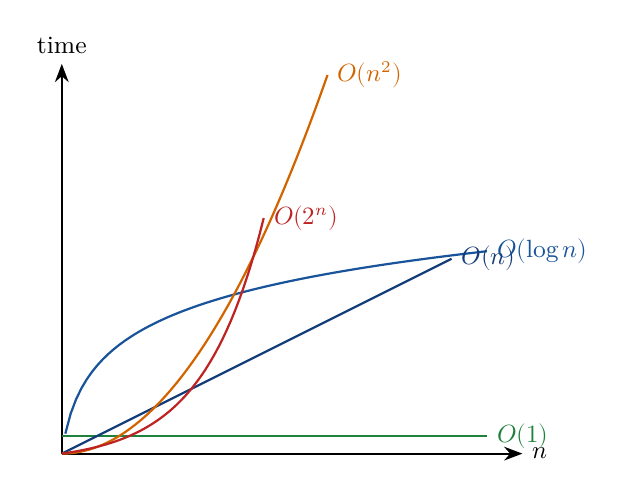
\begin{tikzpicture}[scale=0.9]
  \draw[-{Stealth}, thick] (0,0) -- (6.5,0) node[right]{\small $n$};
  \draw[-{Stealth}, thick] (0,0) -- (0,5.5) node[above]{\small time};
  % O(1)
  \draw[mygreen,   thick] (0,0.25) -- (6,0.25)
    node[right, font=\small, mygreen]{$O(1)$};
  % O(log n)
  \draw[mybluelt,  thick, domain=0.05:6, samples=80]
    plot (\x, {1.6*ln(10*\x+1)/ln(10)})
    node[right, font=\small, mybluelt]{$O(\log n)$};
  % O(n)
  \draw[myblue,    thick] (0,0) -- (5.5, 2.75)
    node[right, font=\small, myblue]{$O(n)$};
  % O(n^2)
  \draw[myorange,  thick, domain=0:3.75, samples=60]
    plot (\x, {0.38*\x*\x})
    node[right, font=\small, myorange]{$O(n^2)$};
  % O(2^n) clipped
  \draw[myred,     thick, domain=0:2.85, samples=50]
    plot (\x, {0.12*(2^(1.7*\x)-1)})
    node[right, font=\small, myred]{$O(2^n)$};
\end{tikzpicture}
\end{center}

\section{Rules for Analysing Code}

\begin{enumerate}
  \item \textbf{Any single statement} (assignment, print, return) $\to O(1)$
  \item \textbf{A loop running $n$ times} with $O(1)$ body $\to O(n)$
  \item \textbf{Two nested loops, each $n$ times} $\to O(n^2)$
  \item \textbf{Two sequential (non-nested) blocks}: add them, keep the dominant term
  \item \textbf{Input is halved each step} (binary search, etc.) $\to O(\log n)$
\end{enumerate}

\begin{lstlisting}[caption={Identifying complexity from code structure}]
// O(1): single operation, no loop
int getFirst(int[] arr) {
    return arr[0];
}

// O(n): one loop over n elements
int sumArray(int[] arr) {
    int sum = 0;                          // O(1)
    for (int i = 0; i < arr.length; i++) // n iterations
        sum += arr[i];                    // O(1) per iteration
    return sum;                           // O(1)
}   // Total: O(n)

// O(n^2): nested loops
void printAllPairs(int[] arr) {
    int n = arr.length;
    for (int i = 0; i < n; i++)          // n iterations
        for (int j = 0; j < n; j++)      // n iterations each
            System.out.print(arr[i] + "," + arr[j] + " ");
}   // Total: n * n = O(n^2)
\end{lstlisting}

\section{Space Complexity}

\begin{definitionbox}{Space Complexity}
The amount of \textbf{extra memory} an algorithm uses, beyond its input.
\begin{itemize}
  \item $O(1)$ --- Only a fixed number of variables (int, double, etc.)
  \item $O(n)$ --- An extra array or list of size $n$
  \item $O(n^2)$ --- A 2-D matrix of size $n \times n$
\end{itemize}
The input itself is not counted --- only the \textit{additional} memory you allocate.
\end{definitionbox}

\begin{interviewcorner}
\begin{itemize}
  \item Always mention \textbf{both} Time \textbf{and} Space complexity
  \item ``$O(n^2)$ solution'' is acceptable when $n \leq 1000$
  \item For $n \leq 10^6$, aim for $O(n \log n)$ or better
  \item When asked ``Can you optimise?'' --- the interviewer usually wants $O(n)$
  \item Trading space for time (and vice versa) is a valid interview discussion
\end{itemize}
\end{interviewcorner}

%%############################################################
\chapter{Basic Mathematics for DSA}
%%############################################################

These problems appear directly in DSA interviews and also build the maths intuition needed for harder problems.

\section{Count Digits of a Number}

\textbf{Problem:} Given integer $n$, count how many digits it has.

\textbf{Idea:} Keep dividing by 10 until the number becomes 0. Each division removes one digit.

\begin{lstlisting}[caption={Count Digits --- Loop method}]
public class CountDigits {
    public static int countDigits(int n) {
        if (n == 0) return 1;          // special case: 0 has 1 digit
        int count = 0;
        n = Math.abs(n);               // handle negatives

        while (n > 0) {
            n = n / 10;                // remove last digit
            count++;                   // count this digit
        }
        return count;
    }

    public static void main(String[] args) {
        System.out.println(countDigits(12345)); // 5
        System.out.println(countDigits(0));     // 1
        System.out.println(countDigits(-987));  // 3
    }
}
\end{lstlisting}

\begin{dryrun}[Dry Run: countDigits(12345)]
\begin{center}
\begin{tabular}{cccc}
\toprule
\textbf{Iteration} & \textbf{n (before)} & \textbf{n = n / 10} & \textbf{count}\\
\midrule
1 & 12345 & 1234 & 1\\
2 & 1234  & 123  & 2\\
3 & 123   & 12   & 3\\
4 & 12    & 1    & 4\\
5 & 1     & 0    & 5\\
\multicolumn{3}{l}{n = 0, loop ends} & 5\\
\bottomrule
\end{tabular}
\end{center}
\textbf{Result: 5 digits}
\end{dryrun}

\begin{complexity}
Time: $O(\log_{10} n)$ --- one iteration per digit\quad Space: $O(1)$
\end{complexity}

\section{Reverse a Number}

\textbf{Idea:} Extract the last digit using \texttt{\% 10}, append it to the result, remove it with \texttt{/ 10}.

\begin{lstlisting}[caption={Reverse a Number}]
public class ReverseNumber {
    public static int reverse(int n) {
        int reversed = 0;
        n = Math.abs(n);               // handle negatives

        while (n > 0) {
            int lastDigit = n % 10;               // extract last digit
            reversed = reversed * 10 + lastDigit; // shift and append
            n = n / 10;                           // remove last digit
        }
        return reversed;
    }

    public static void main(String[] args) {
        System.out.println(reverse(12345)); // 54321
        System.out.println(reverse(100));   // 1
    }
}
\end{lstlisting}

\begin{dryrun}[Dry Run: reverse(1234)]
\begin{center}
\begin{tabular}{ccccc}
\toprule
\textbf{Step} & \textbf{n} & \textbf{lastDigit (n \% 10)} & \textbf{reversed} & \textbf{n after / 10}\\
\midrule
1 & 1234 & 4 & $0 \times 10 + 4 = 4$    & 123\\
2 & 123  & 3 & $4 \times 10 + 3 = 43$   & 12\\
3 & 12   & 2 & $43 \times 10 + 2 = 432$ & 1\\
4 & 1    & 1 & $432 \times 10 + 1 = 4321$ & 0\\
\bottomrule
\end{tabular}
\end{center}
\textbf{Result: 4321}
\end{dryrun}

\section{Palindrome Number}

A number is a \textbf{palindrome} if it reads the same forwards and backwards (e.g., 121, 1221, 12321).

\begin{lstlisting}[caption={Check Palindrome Number}]
public class PalindromeCheck {
    public static boolean isPalindrome(int n) {
        if (n < 0) return false;       // negatives are never palindromes

        int original = n;
        int reversed = 0;

        while (n > 0) {
            reversed = reversed * 10 + (n % 10);
            n = n / 10;
        }
        return original == reversed;
    }

    public static void main(String[] args) {
        System.out.println(isPalindrome(121));   // true
        System.out.println(isPalindrome(123));   // false
        System.out.println(isPalindrome(1221));  // true
    }
}
\end{lstlisting}

\begin{complexity}
Time: $O(\log_{10} n)$\quad Space: $O(1)$
\end{complexity}

\section{Factorial of a Number}

$n! = n \times (n-1) \times (n-2) \times \cdots \times 2 \times 1$, with $0! = 1$.

\begin{lstlisting}[caption={Factorial --- Iterative approach}]
public class Factorial {
    public static long factorial(int n) {
        if (n < 0) return -1;         // factorial undefined for negatives
        long result = 1;
        for (int i = 2; i <= n; i++) {
            result = result * i;
        }
        return result;
    }

    public static void main(String[] args) {
        System.out.println(factorial(5));  // 120  (5*4*3*2*1)
        System.out.println(factorial(0));  // 1
        System.out.println(factorial(10)); // 3628800
    }
}
\end{lstlisting}

\begin{tipbox}[Use \texttt{long} for Factorial]
\texttt{int} overflows at $n = 13$ ($13! = 6{,}227{,}020{,}800 > 2.1$B). Use \texttt{long} to handle up to $n = 20$. For $n > 20$, use \texttt{BigInteger}.
\end{tipbox}

\section{GCD and LCM}

\textbf{GCD} (Greatest Common Divisor) --- the largest integer that divides both $a$ and $b$ without remainder.

\textbf{LCM} (Lowest Common Multiple) --- the smallest positive integer divisible by both.

\textbf{Relationship:} $\text{LCM}(a,b) \times \text{GCD}(a,b) = a \times b$

\textbf{Euclidean Algorithm:} $\gcd(a, b) = \gcd(b,\; a \bmod b)$, stop when $b = 0$.

\begin{lstlisting}[caption={GCD and LCM using Euclidean Algorithm}]
public class GcdLcm {
    public static int gcd(int a, int b) {
        while (b != 0) {
            int temp = b;
            b = a % b;     // b becomes the remainder
            a = temp;      // a becomes the old b
        }
        return a;          // when b = 0, a holds the GCD
    }

    public static int lcm(int a, int b) {
        // Divide first to avoid integer overflow
        return (a / gcd(a, b)) * b;
    }

    public static void main(String[] args) {
        System.out.println("GCD(12, 8) = " + gcd(12, 8));  // 4
        System.out.println("LCM(12, 8) = " + lcm(12, 8));  // 24
    }
}
\end{lstlisting}

\begin{dryrun}[Dry Run: gcd(12, 8)]
\begin{center}
\begin{tabular}{cccc}
\toprule
\textbf{Step} & \textbf{a} & \textbf{b} & \textbf{b = a \% b}\\
\midrule
1 & 12 & 8 & $12 \% 8 = 4$\\
2 & 8  & 4 & $8 \% 4 = 0$\\
3 & 4  & 0 & Loop ends\\
\bottomrule
\end{tabular}
\end{center}
\textbf{Result:} GCD = 4, so LCM = $(12 / 4) \times 8 = 24$
\end{dryrun}

\begin{complexity}
Time: $O(\log \min(a,b))$ --- the Euclidean algorithm is very fast\quad Space: $O(1)$
\end{complexity}

\section{Prime Number Check}

A number $n$ is \textbf{prime} if it has exactly two divisors: 1 and itself. (1 is not prime; 2 is the only even prime.)

\begin{lstlisting}[caption={Is Prime? --- Optimised $O(\sqrt{n})$ check}]
public class PrimeCheck {
    public static boolean isPrime(int n) {
        if (n <= 1) return false;           // 0 and 1 are not prime
        if (n == 2) return true;            // 2 is prime
        if (n % 2 == 0) return false;       // all other even numbers: not prime

        // Check odd divisors from 3 up to sqrt(n)
        for (int i = 3; i * i <= n; i += 2) {
            if (n % i == 0) return false;   // found a divisor
        }
        return true;
    }

    public static void main(String[] args) {
        System.out.println(isPrime(7));    // true
        System.out.println(isPrime(12));   // false
        System.out.println(isPrime(97));   // true
    }
}
\end{lstlisting}

\begin{tipbox}[Why check only up to $\sqrt{n}$?]
If $n$ has a divisor $d > \sqrt{n}$, then $n/d < \sqrt{n}$ is also a divisor --- and we would have already found it. So we never need to check beyond $\sqrt{n}$.

Example: $n = 36$. Divisors: 1, 2, 3, 4, \textbf{6}, 9, 12, 18, 36. $\sqrt{36} = 6$. All divisors $> 6$ pair with one $\leq 6$.
\end{tipbox}

\begin{complexity}
Naive: $O(n)$\quad Optimised: $O(\sqrt{n})$. For $n = 10^{12}$: from $10^{12}$ ops down to $10^6$ ops.
\end{complexity}

%%############################################################
\chapter{1-D Arrays}
%%############################################################

Arrays are the single most important topic for DSA interviews. Nearly every other data structure (stack, queue, heap, hash table) is implemented using arrays internally.

\section{What is an Array?}

\begin{definitionbox}{Array}
An \textbf{array} is a collection of elements of the \textbf{same data type}, stored in \textbf{contiguous (adjacent) memory locations}, each accessible in $O(1)$ time via a 0-based \textbf{index}.
\end{definitionbox}

\subsection{Memory Representation}

\begin{center}
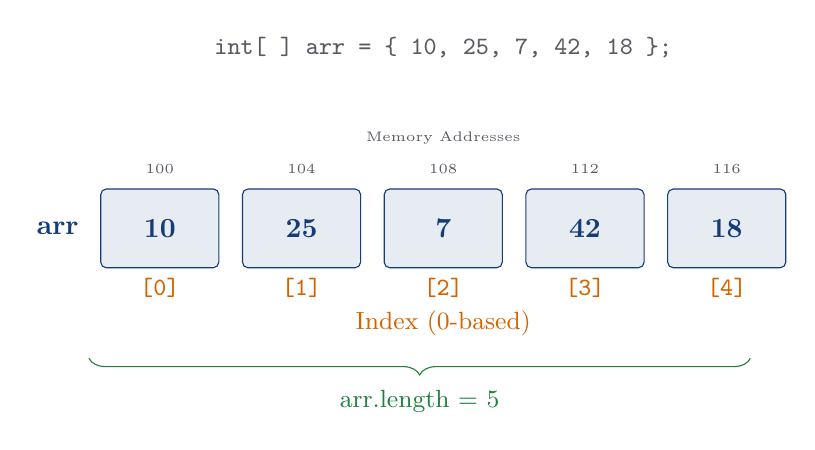
\begin{tikzpicture}[font=\small]
  % declaration label
  \node[text=mygray, font=\ttfamily\small] at (3.6, 2.3)
    {int[ ] arr = \{ 10,\ 25,\ 7,\ 42,\ 18 \};};

  % memory cells
  \foreach \v/\i/\addr in {10/0/100, 25/1/104, 7/2/108, 42/3/112, 18/4/116}{
    \node[draw=myblue, fill=myblue!10,
          minimum width=1.5cm, minimum height=1.0cm,
          font=\bfseries, text=myblue, rounded corners=2pt]
      (cell\i) at (\i*1.8, 0) {\v};
    \node[text=myorange, font=\ttfamily\small] at (\i*1.8, -0.75) {[\i]};
    \node[text=mygray, font=\tiny]             at (\i*1.8, 0.75)  {\addr};
  }

  \node[text=myblue, left=0.15cm of cell0, font=\bfseries] {arr};
  \node[text=mygray, font=\tiny] at (3.6, 1.15) {Memory Addresses};
  \node[text=myorange, font=\small] at (3.6, -1.2) {Index (0-based)};

  % brace
  \draw[mygreen, decorate,
        decoration={brace, amplitude=6pt, mirror}]
    (-0.9, -1.65) -- (7.5, -1.65)
    node[midway, below=8pt, text=mygreen, font=\small]
      {arr.length = 5};
\end{tikzpicture}
\end{center}

\textbf{Key Properties:}
\begin{itemize}
  \item \textbf{Fixed size} --- Size is set at creation; cannot grow or shrink
  \item \textbf{0-indexed} --- First element is at index \texttt{0}; last is at index \texttt{arr.length - 1}
  \item \textbf{$O(1)$ random access} --- Any element can be read or written in constant time
  \item \textbf{Same type} --- All elements share one data type
  \item \textbf{Contiguous memory} --- Elements sit side-by-side in RAM (cache-friendly)
\end{itemize}

\section{Declaring and Initialising Arrays}

\begin{lstlisting}[caption={All ways to declare and initialise arrays in Java}]
public class ArrayDeclaration {
    public static void main(String[] args) {

        // WAY 1: Declare size only -- JVM fills with default values
        //   int  -> 0,  double -> 0.0,  boolean -> false,  String -> null
        int[] arr1 = new int[5];         // {0, 0, 0, 0, 0}

        // WAY 2: Declare with values -- compiler counts the size
        int[] arr2 = {10, 20, 30, 40, 50};

        // WAY 3: new keyword with values (same result as Way 2)
        int[] arr3 = new int[]{10, 20, 30, 40, 50};

        // ---------- Accessing elements ----------
        System.out.println(arr2[0]);   // 10  (first element, index 0)
        System.out.println(arr2[4]);   // 50  (last element, index 4)

        // arr2[5] -> ArrayIndexOutOfBoundsException (out of range!)

        // ---------- Modifying an element ----------
        arr2[2] = 99;
        System.out.println(arr2[2]);   // 99

        // ---------- Length (PROPERTY, not method - no parentheses!) ----------
        System.out.println("Size = " + arr2.length);        // 5

        // ---------- Last element ----------
        System.out.println("Last = " + arr2[arr2.length - 1]);  // 50
    }
}
\end{lstlisting}

\begin{warningbox}[Most Common Array Mistakes]
\texttt{arr.length} is a \textbf{property} --- no parentheses. Do not write \texttt{arr.length()}.\\
Valid indices: \texttt{0} to \texttt{arr.length - 1}. Accessing \texttt{arr[arr.length]} throws \texttt{ArrayIndexOutOfBoundsException}.
\end{warningbox}

\section{Traversing an Array}

\begin{lstlisting}[caption={Three ways to traverse --- when to use each}]
public class ArrayTraversal {
    public static void main(String[] args) {
        int[] arr = {10, 20, 30, 40, 50};

        // WAY 1: Traditional for loop
        //   Use when: you need the INDEX (most DSA problems)
        System.out.print("for loop : ");
        for (int i = 0; i < arr.length; i++) {
            System.out.print(arr[i] + " ");
        }
        System.out.println();          // Output: 10 20 30 40 50

        // WAY 2: Enhanced for-each loop
        //   Use when: you only need VALUES, not the index (read-only)
        System.out.print("for-each : ");
        for (int x : arr) {
            System.out.print(x + " ");
        }
        System.out.println();          // Output: 10 20 30 40 50

        // WAY 3: while loop
        //   Use when: the traversal condition is complex
        System.out.print("while    : ");
        int i = 0;
        while (i < arr.length) {
            System.out.print(arr[i] + " ");
            i++;
        }
        System.out.println();          // Output: 10 20 30 40 50
    }
}
\end{lstlisting}

\section{Sum of Array Elements}

\begin{lstlisting}[caption={Sum of all elements --- accumulator pattern}]
public class ArraySum {
    public static int sumArray(int[] arr) {
        int sum = 0;
        for (int i = 0; i < arr.length; i++) {
            sum = sum + arr[i];   // add current element to running total
        }
        return sum;
    }

    public static void main(String[] args) {
        int[] arr = {3, 1, 4, 1, 5, 9, 2, 6};
        System.out.println("Sum = " + sumArray(arr));  // 31
    }
}
\end{lstlisting}

\begin{dryrun}[Dry Run: arr = \{3, 1, 4, 1, 5\}]
\begin{center}
\begin{tabular}{cccc}
\toprule
\textbf{i} & \textbf{arr[i]} & \textbf{sum (before)} & \textbf{sum (after)}\\
\midrule
0 & 3 & 0  & 3\\
1 & 1 & 3  & 4\\
2 & 4 & 4  & 8\\
3 & 1 & 8  & 9\\
4 & 5 & 9  & 14\\
\bottomrule
\end{tabular}
\end{center}
\textbf{Result: 14}
\end{dryrun}

\begin{complexity}
Time: $O(n)$ --- visit every element once\quad Space: $O(1)$ --- only \texttt{sum} variable
\end{complexity}

\section{Largest and Smallest Element}

\begin{lstlisting}[caption={Find Max and Min in a single pass each}]
public class MaxMin {
    public static int findMax(int[] arr) {
        int max = arr[0];                 // assume first element is max
        for (int i = 1; i < arr.length; i++) {
            if (arr[i] > max) {
                max = arr[i];             // update when a larger value found
            }
        }
        return max;
    }

    public static int findMin(int[] arr) {
        int min = arr[0];
        for (int i = 1; i < arr.length; i++) {
            if (arr[i] < min) {
                min = arr[i];
            }
        }
        return min;
    }

    public static void main(String[] args) {
        int[] arr = {64, 34, 25, 12, 22, 11, 90};
        System.out.println("Max = " + findMax(arr));  // 90
        System.out.println("Min = " + findMin(arr));  // 11
    }
}
\end{lstlisting}

\begin{dryrun}[Dry Run: findMax on \{64, 34, 25, 12, 22, 11, 90\}]
\begin{center}
\begin{tabular}{cccl}
\toprule
\textbf{i} & \textbf{arr[i]} & \textbf{max} & \textbf{Updated?}\\
\midrule
init& ---  & 64 & max = arr[0] = 64\\
1   & 34   & 64 & $34 > 64$? No\\
2   & 25   & 64 & $25 > 64$? No\\
3   & 12   & 64 & $12 > 64$? No\\
4   & 22   & 64 & $22 > 64$? No\\
5   & 11   & 64 & $11 > 64$? No\\
6   & 90   & \textbf{90} & $90 > 64$? \textbf{Yes} $\to$ max = 90\\
\bottomrule
\end{tabular}
\end{center}
\textbf{Result: max = 90}
\end{dryrun}

\begin{complexity}
Time: $O(n)$\quad Space: $O(1)$
\end{complexity}

\section{Second Largest Element}

Find the second largest without sorting --- in a single pass.

\begin{lstlisting}[caption={Second Largest --- Single Pass $O(n)$}]
public class SecondLargest {
    public static int secondLargest(int[] arr) {
        if (arr.length < 2) return -1;    // not enough elements

        int first  = Integer.MIN_VALUE;   // will hold the largest
        int second = Integer.MIN_VALUE;   // will hold second largest

        for (int i = 0; i < arr.length; i++) {
            if (arr[i] > first) {
                second = first;           // old largest drops to second place
                first  = arr[i];          // new largest found
            } else if (arr[i] > second && arr[i] != first) {
                second = arr[i];          // update second (skip duplicates of first)
            }
        }
        if (second == Integer.MIN_VALUE) return -1;  // all elements identical
        return second;
    }

    public static void main(String[] args) {
        int[] arr = {12, 35, 1, 10, 34, 1};
        System.out.println(secondLargest(arr));  // 34
    }
}
\end{lstlisting}

\begin{dryrun}[Dry Run: arr = \{12, 35, 1, 10, 34, 1\}]
\begin{center}
\begin{tabular}{cccc}
\toprule
\textbf{i} & \textbf{arr[i]} & \textbf{first} & \textbf{second}\\
\midrule
init & ---& MIN\_VALUE & MIN\_VALUE\\
0    & 12 & 12         & MIN\_VALUE\\
1    & 35 & 35         & 12\\
2    & 1  & 35         & 12\\
3    & 10 & 35         & 12\\
4    & 34 & 35         & \textbf{34}\\
5    & 1  & 35         & 34\\
\bottomrule
\end{tabular}
\end{center}
\textbf{Result: 34}
\end{dryrun}

\begin{complexity}
Time: $O(n)$ --- single pass\quad Space: $O(1)$
\end{complexity}

\section{Linear Search}

\textbf{Problem:} Search for a target value. Return its index, or $-1$ if not found.

\begin{lstlisting}[caption={Linear Search --- scan left to right}]
public class LinearSearch {
    public static int linearSearch(int[] arr, int target) {
        for (int i = 0; i < arr.length; i++) {
            if (arr[i] == target) {
                return i;      // found! return the index
            }
        }
        return -1;             // target not in array
    }

    public static void main(String[] args) {
        int[] arr = {10, 23, 45, 70, 11, 15};
        System.out.println(linearSearch(arr, 70));  //  3
        System.out.println(linearSearch(arr, 99));  // -1
    }
}
\end{lstlisting}

\begin{center}
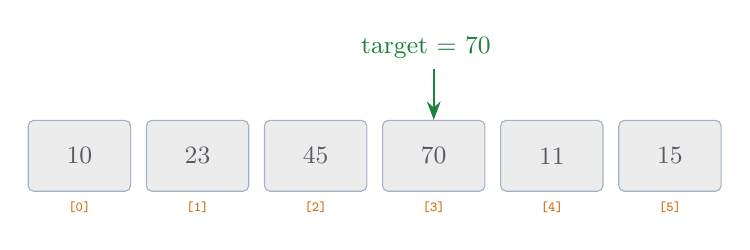
\begin{tikzpicture}[font=\small]
  \foreach \v/\i/\found in {10/0/n, 23/1/n, 45/2/n, 70/3/y, 11/4/n, 15/5/n}{
    \ifx\found y
      \node[draw=mygreen, fill=mygreen!10, minimum width=1.3cm,
            minimum height=0.9cm, font=\bfseries, text=mygreen,
            rounded corners=2pt](cell\i) at (\i*1.5, 0){\v};
    \else
      \node[draw=myblue!40, fill=gray!15, minimum width=1.3cm,
            minimum height=0.9cm, text=mygray,
            rounded corners=2pt](cell\i) at (\i*1.5, 0){\v};
    \fi
    \node[text=myorange, font=\tiny\ttfamily] at (\i*1.5,-0.65){[\i]};
  }
  \draw[mygreen,-{Stealth},thick](4.5,1.1)
    node[above,text=mygreen,font=\small]{target = 70\ \checkmark}
    -- (cell3.north);
\end{tikzpicture}
\end{center}

\begin{complexity}
Best: $O(1)$ (found at index 0)\quad Worst: $O(n)$ (last or not present)\quad Space: $O(1)$
\end{complexity}

\section{Check if Array is Sorted}

\begin{lstlisting}[caption={Is the array sorted in ascending order?}]
public class IsSorted {
    public static boolean isSorted(int[] arr) {
        // Compare every adjacent pair; if any pair violates order, return false
        for (int i = 0; i < arr.length - 1; i++) {
            if (arr[i] > arr[i + 1]) {
                return false;    // found a descending pair -- not sorted
            }
        }
        return true;             // no violations found
    }

    public static void main(String[] args) {
        int[] a = {1, 2, 3, 4, 5};
        int[] b = {1, 3, 2, 4, 5};   // 3 > 2: violation at index 1-2
        System.out.println(isSorted(a));  // true
        System.out.println(isSorted(b));  // false
    }
}
\end{lstlisting}

\begin{complexity}
Time: $O(n)$\quad Space: $O(1)$
\end{complexity}

\section{Reverse an Array}

\textbf{Approach:} Two-pointer technique. Place one pointer at the start (\texttt{left}) and one at the end (\texttt{right}). Swap and move both inward until they meet.

\begin{lstlisting}[caption={Reverse Array --- Two Pointer, in-place}]
public class ReverseArray {
    public static void reverse(int[] arr) {
        int left  = 0;
        int right = arr.length - 1;

        while (left < right) {
            // Swap arr[left] and arr[right]
            int temp    = arr[left];
            arr[left]   = arr[right];
            arr[right]  = temp;

            left++;    // move left pointer rightward
            right--;   // move right pointer leftward
        }
    }

    public static void main(String[] args) {
        int[] arr = {1, 2, 3, 4, 5};
        System.out.print("Before: ");
        for (int x : arr) System.out.print(x + " ");

        reverse(arr);

        System.out.print("\nAfter:  ");
        for (int x : arr) System.out.print(x + " ");
        // Output Before: 1 2 3 4 5
        // Output After:  5 4 3 2 1
    }
}
\end{lstlisting}

\begin{dryrun}[Dry Run: reverse(\{1, 2, 3, 4, 5\})]
\begin{center}
\begin{tabular}{ccccc}
\toprule
\textbf{Step} & \textbf{left} & \textbf{right} & \textbf{Swap} & \textbf{Array State}\\
\midrule
Start  & 0 & 4 & ---                             & \{1, 2, 3, 4, 5\}\\
1      & 0 & 4 & arr[0] $\leftrightarrow$ arr[4] & \{5, 2, 3, 4, 1\}\\
2      & 1 & 3 & arr[1] $\leftrightarrow$ arr[3] & \{5, 4, 3, 2, 1\}\\
3      & 2 & 2 & left $\not<$ right: \textbf{stop}& \{5, 4, 3, 2, 1\}\\
\bottomrule
\end{tabular}
\end{center}
\textbf{Result: \{5, 4, 3, 2, 1\}}
\end{dryrun}

\begin{center}
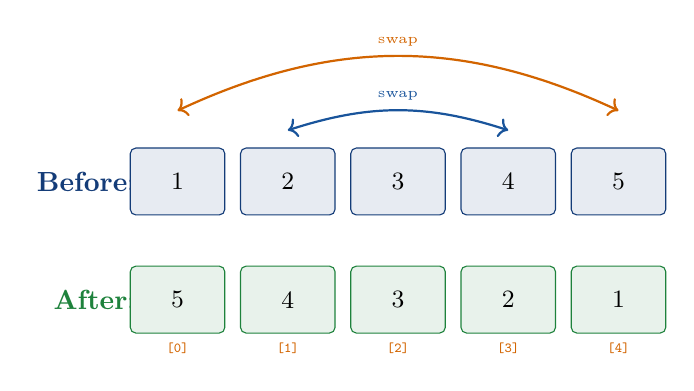
\begin{tikzpicture}[font=\small]
  \node[left, text=myblue, font=\bfseries] at (-0.4, 1.5){Before:};
  \foreach \v/\i in {1/0, 2/1, 3/2, 4/3, 5/4}{
    \node[draw=myblue, fill=myblue!10, minimum width=1.2cm,
          minimum height=0.85cm, rounded corners=2pt]
      at (\i*1.4, 1.5){\v};
  }
  \draw[myorange, <->, thick, bend left=25] (0, 2.4) to
    node[above, font=\tiny, myorange]{swap} (5.6, 2.4);
  \draw[mybluelt, <->, thick, bend left=18] (1.4, 2.15) to
    node[above, font=\tiny, mybluelt]{swap} (4.2, 2.15);

  \node[left, text=mygreen, font=\bfseries] at (-0.4, 0){After:};
  \foreach \v/\i in {5/0, 4/1, 3/2, 2/3, 1/4}{
    \node[draw=mygreen, fill=mygreen!10, minimum width=1.2cm,
          minimum height=0.85cm, rounded corners=2pt]
      at (\i*1.4, 0){\v};
    \node[text=myorange, font=\tiny\ttfamily] at (\i*1.4,-0.62){[\i]};
  }
\end{tikzpicture}
\end{center}

\begin{complexity}
Time: $O(n)$ --- $\lfloor n/2 \rfloor$ swaps\quad Space: $O(1)$ --- in-place, only \texttt{temp}
\end{complexity}

\section{Count Odd Numbers in Array}

\begin{lstlisting}[caption={Count all odd elements}]
public class CountOdd {
    public static int countOdd(int[] arr) {
        int count = 0;
        for (int i = 0; i < arr.length; i++) {
            if (arr[i] % 2 != 0) {    // odd: remainder when divided by 2 is 1
                count++;
            }
        }
        return count;
    }

    public static void main(String[] args) {
        int[] arr = {1, 2, 3, 4, 5, 6, 7, 8};
        System.out.println("Odd count = " + countOdd(arr));  // 4
    }
}
\end{lstlisting}

\begin{complexity}
Time: $O(n)$\quad Space: $O(1)$
\end{complexity}

\section{Left Rotate Array by One}

\begin{lstlisting}[caption={Left Rotate by One Position}]
public class RotateByOne {
    public static void rotateByOne(int[] arr) {
        int n     = arr.length;
        int first = arr[0];          // save the first element

        // shift every element one index to the left
        for (int i = 0; i < n - 1; i++) {
            arr[i] = arr[i + 1];
        }
        arr[n - 1] = first;          // place saved element at the end
    }

    public static void main(String[] args) {
        int[] arr = {1, 2, 3, 4, 5};
        System.out.print("Before: ");
        for (int x : arr) System.out.print(x + " ");   // 1 2 3 4 5

        rotateByOne(arr);

        System.out.print("\nAfter:  ");
        for (int x : arr) System.out.print(x + " ");   // 2 3 4 5 1
    }
}
\end{lstlisting}

\begin{dryrun}[Dry Run: arr = \{1, 2, 3, 4, 5\}]
\begin{center}
\begin{tabular}{lll}
\toprule
\textbf{Action} & \textbf{Array State} & \textbf{Notes}\\
\midrule
Initial             & \{1, 2, 3, 4, 5\} & first = 1 (saved)\\
After shift loop    & \{2, 3, 4, 5, 5\} & each element moved left\\
After arr[4] = 1    & \{2, 3, 4, 5, 1\} & saved element placed at end\\
\bottomrule
\end{tabular}
\end{center}
\textbf{Result: \{2, 3, 4, 5, 1\}}
\end{dryrun}

\begin{complexity}
Time: $O(n)$\quad Space: $O(1)$
\end{complexity}

\section{Left Rotate by K Places}

\textbf{Approach: Triple Reverse Trick}

To rotate left by $k$:
\begin{enumerate}
  \item Reverse the first $k$ elements
  \item Reverse the remaining $n-k$ elements
  \item Reverse the entire array
\end{enumerate}

\begin{lstlisting}[caption={Left Rotate by K --- Triple Reverse, O(n) time O(1) space}]
public class RotateByK {
    // Helper: reverse arr[start..end] in-place
    private static void reverse(int[] arr, int start, int end) {
        while (start < end) {
            int temp       = arr[start];
            arr[start]     = arr[end];
            arr[end]       = temp;
            start++;
            end--;
        }
    }

    public static void rotateLeft(int[] arr, int k) {
        int n = arr.length;
        k = k % n;             // e.g., k=7, n=5 -> k=2 (same effect)
        if (k == 0) return;    // nothing to rotate

        reverse(arr, 0, k - 1);    // Step 1: reverse first k elements
        reverse(arr, k, n - 1);    // Step 2: reverse remaining n-k elements
        reverse(arr, 0, n - 1);    // Step 3: reverse the whole array
    }

    public static void main(String[] args) {
        int[] arr = {1, 2, 3, 4, 5};
        rotateLeft(arr, 2);
        for (int x : arr) System.out.print(x + " ");
        // Output: 3 4 5 1 2
    }
}
\end{lstlisting}

\begin{dryrun}[Dry Run: arr = \{1, 2, 3, 4, 5\}, k = 2]
\begin{center}
\begin{tabular}{ll}
\toprule
\textbf{Step} & \textbf{Array State}\\
\midrule
Initial                       & \{1, 2, 3, 4, 5\}\\
Reverse arr[0..1]             & \{2, 1, 3, 4, 5\}\\
Reverse arr[2..4]             & \{2, 1, 5, 4, 3\}\\
Reverse arr[0..4] (whole)     & \{3, 4, 5, 1, 2\}\\
\bottomrule
\end{tabular}
\end{center}
\textbf{Result: \{3, 4, 5, 1, 2\}} --- elements at positions 0 and 1 moved to the end.
\end{dryrun}

\begin{complexity}
Time: $O(n)$ --- three reversals each $O(n)$\quad Space: $O(1)$ --- completely in-place
\end{complexity}

\begin{interviewcorner}
Also know the \textbf{extra-array approach}: copy the last $n-k$ elements to a temp array, then the first $k$ elements, then copy back. It is $O(n)$ time but $O(n)$ space --- worse in space. The triple-reverse trick is the optimal solution.
\end{interviewcorner}

\section{Maximum Consecutive Ones}

\textbf{Problem:} Given a binary array (only 0s and 1s), find the length of the longest consecutive run of 1s.

\begin{lstlisting}[caption={Maximum Consecutive Ones --- streak counter}]
public class MaxConsecutiveOnes {
    public static int maxOnes(int[] arr) {
        int maxCount = 0;   // best streak seen so far
        int count    = 0;   // current streak length

        for (int i = 0; i < arr.length; i++) {
            if (arr[i] == 1) {
                count++;                              // extend the streak
                maxCount = Math.max(maxCount, count); // update best
            } else {
                count = 0;    // 0 breaks the streak; reset
            }
        }
        return maxCount;
    }

    public static void main(String[] args) {
        int[] arr = {1, 1, 0, 1, 1, 1, 0, 1};
        System.out.println(maxOnes(arr));  // 3
    }
}
\end{lstlisting}

\begin{dryrun}[Dry Run: arr = \{1, 1, 0, 1, 1, 1, 0, 1\}]
\begin{center}
\begin{tabular}{ccccl}
\toprule
\textbf{i} & \textbf{arr[i]} & \textbf{count} & \textbf{maxCount} & \textbf{Note}\\
\midrule
0 & 1 & 1 & 1 & streak starts\\
1 & 1 & 2 & 2 & streak extends\\
2 & 0 & 0 & 2 & reset on 0\\
3 & 1 & 1 & 2 & new streak\\
4 & 1 & 2 & 2 & extends\\
5 & 1 & 3 & \textbf{3} & new best!\\
6 & 0 & 0 & 3 & reset on 0\\
7 & 1 & 1 & 3 & streak, max stays 3\\
\bottomrule
\end{tabular}
\end{center}
\textbf{Result: 3}
\end{dryrun}

\begin{complexity}
Time: $O(n)$\quad Space: $O(1)$
\end{complexity}

\section{Move Zeros to End}

\textbf{Problem:} Move all zeros to the end while preserving the \textbf{relative order} of non-zero elements.

\begin{lstlisting}[caption={Move Zeros to End --- Two Pointer, O(n) O(1)}]
public class MoveZeros {
    public static void moveZeros(int[] arr) {
        int j = 0;    // j = index where the next non-zero element goes

        // Pass 1: push all non-zeros to the front
        for (int i = 0; i < arr.length; i++) {
            if (arr[i] != 0) {
                arr[j] = arr[i];   // place non-zero at position j
                j++;
            }
            // if arr[i] == 0: skip it
        }

        // Pass 2: fill remaining positions (j to end) with zeros
        while (j < arr.length) {
            arr[j] = 0;
            j++;
        }
    }

    public static void main(String[] args) {
        int[] arr = {0, 1, 0, 3, 12};
        moveZeros(arr);
        for (int x : arr) System.out.print(x + " ");
        // Output: 1 3 12 0 0
    }
}
\end{lstlisting}

\begin{dryrun}[Dry Run: arr = \{0, 1, 0, 3, 12\}]
\begin{center}
\begin{tabular}{ccccl}
\toprule
\textbf{i} & \textbf{arr[i]} & \textbf{j (before)} & \textbf{j (after)} & \textbf{Action}\\
\midrule
0 & 0  & 0 & 0 & Skip (zero)\\
1 & 1  & 0 & 1 & arr[0] = 1\\
2 & 0  & 1 & 1 & Skip (zero)\\
3 & 3  & 1 & 2 & arr[1] = 3\\
4 & 12 & 2 & 3 & arr[2] = 12\\
\midrule
\multicolumn{5}{l}{Fill: arr[3] = 0, arr[4] = 0 $\to$ \{1, 3, 12, 0, 0\}}\\
\bottomrule
\end{tabular}
\end{center}
\end{dryrun}

\begin{complexity}
Time: $O(n)$\quad Space: $O(1)$
\end{complexity}

\section{Remove Duplicates from Sorted Array}

\textbf{Problem:} Given a \textbf{sorted} array, remove duplicates in-place. Return the count of unique elements.

\begin{lstlisting}[caption={Remove Duplicates from Sorted Array --- Two Pointer}]
public class RemoveDuplicates {
    public static int removeDuplicates(int[] arr) {
        if (arr.length == 0) return 0;

        int j = 0;    // j points to the last unique element placed

        for (int i = 1; i < arr.length; i++) {
            if (arr[i] != arr[j]) {    // found a new unique element
                j++;                   // move j forward
                arr[j] = arr[i];       // place it at the next unique position
            }
            // if arr[i] == arr[j]: it's a duplicate -- skip it
        }
        return j + 1;  // unique count: indices 0 through j
    }

    public static void main(String[] args) {
        int[] arr = {1, 1, 2, 2, 3, 4, 4, 5};
        int uniqueLen = removeDuplicates(arr);

        System.out.print("Unique elements: ");
        for (int i = 0; i < uniqueLen; i++) {
            System.out.print(arr[i] + " ");
        }
        // Output: 1 2 3 4 5
    }
}
\end{lstlisting}

\begin{dryrun}[Dry Run: arr = \{1, 1, 2, 2, 3\}]
\begin{center}
\begin{tabular}{ccccl}
\toprule
\textbf{i} & \textbf{arr[i]} & \textbf{arr[j]} & \textbf{j} & \textbf{Note}\\
\midrule
init & --- & arr[0]=1 & 0 & Initial state\\
1    & 1   & 1        & 0 & Duplicate, skip\\
2    & 2   & 1        & 1 & Unique! arr[1] = 2\\
3    & 2   & 2        & 1 & Duplicate, skip\\
4    & 3   & 2        & 2 & Unique! arr[2] = 3\\
\bottomrule
\end{tabular}
\end{center}
\textbf{Result: uniqueLen = 3, array front = \{1, 2, 3\}}
\end{dryrun}

\begin{warningbox}[Only Works on Sorted Arrays!]
If the array is unsorted, use a \texttt{LinkedHashSet} to preserve order while removing duplicates, or sort first in $O(n \log n)$.
\end{warningbox}

\begin{complexity}
Time: $O(n)$\quad Space: $O(1)$
\end{complexity}

\section{Find the Missing Number}

\textbf{Problem:} Given an array of $n$ distinct integers from range $[1,\, n]$, exactly one number is missing. Find it.

\begin{lstlisting}[caption={Missing Number --- Sum Formula and XOR (both shown)}]
public class MissingNumber {
    // METHOD 1: Gauss Sum Formula
    //   Expected sum of 1..n = n*(n+1)/2
    //   Missing = expected - actual
    public static int missingBySum(int[] arr) {
        int n           = arr.length + 1;          // total should be n numbers
        int expectedSum = n * (n + 1) / 2;         // Gauss formula
        int actualSum   = 0;
        for (int x : arr) actualSum += x;
        return expectedSum - actualSum;
    }

    // METHOD 2: XOR (preferred -- avoids overflow for very large n)
    //   x ^ x = 0,  x ^ 0 = x
    //   XOR all 1..n with all array values; pairs cancel; missing survives
    public static int missingByXOR(int[] arr) {
        int n      = arr.length + 1;
        int xorAll = 0;
        for (int i = 1; i <= n; i++) xorAll ^= i;   // XOR 1 to n
        for (int x : arr)            xorAll ^= x;   // XOR all array values
        return xorAll;                               // missing number remains
    }

    public static void main(String[] args) {
        int[] arr = {1, 2, 4, 5, 6};    // 3 is missing
        System.out.println(missingBySum(arr));  // 3
        System.out.println(missingByXOR(arr));  // 3
    }
}
\end{lstlisting}

\begin{dryrun}[Sum Method: arr = \{1, 2, 4, 5, 6\}, range [1..6]]
Expected sum $= 6 \times 7 / 2 = 21$\\
Actual sum $= 1 + 2 + 4 + 5 + 6 = 18$\\
Missing $= 21 - 18 = \mathbf{3}$
\end{dryrun}

\begin{complexity}
Time: $O(n)$\quad Space: $O(1)$
\end{complexity}

\begin{interviewcorner}
The \textbf{XOR method} is preferred in interviews because the Gauss sum can overflow \texttt{int} for very large $n$ (e.g., $n = 10^5$ gives sum $\approx 5 \times 10^{9}$, which overflows 32-bit int). Use \texttt{long} with the sum method as a safe alternative. XOR has no overflow risk.
\end{interviewcorner}

\section{Union of Two Sorted Arrays}

\textbf{Problem:} Return a sorted array containing every unique element from both sorted arrays.

\begin{lstlisting}[caption={Union of Two Sorted Arrays --- Two Pointer, O(m+n)}]
import java.util.ArrayList;

public class UnionArrays {
    public static ArrayList<Integer> union(int[] a, int[] b) {
        ArrayList<Integer> res = new ArrayList<>();
        int i = 0, j = 0;

        while (i < a.length && j < b.length) {
            // Skip duplicates already added to result
            if (!res.isEmpty() && res.get(res.size() - 1) == a[i]) { i++; continue; }
            if (!res.isEmpty() && res.get(res.size() - 1) == b[j]) { j++; continue; }

            if      (a[i] < b[j]) res.add(a[i++]);
            else if (a[i] > b[j]) res.add(b[j++]);
            else                { res.add(a[i]); i++; j++; } // both equal
        }
        // Drain remaining elements from a
        while (i < a.length) {
            if (res.isEmpty() || res.get(res.size()-1) != a[i]) res.add(a[i]);
            i++;
        }
        // Drain remaining elements from b
        while (j < b.length) {
            if (res.isEmpty() || res.get(res.size()-1) != b[j]) res.add(b[j]);
            j++;
        }
        return res;
    }

    public static void main(String[] args) {
        int[] a = {1, 2, 3, 4, 5};
        int[] b = {1, 2, 3, 6, 7};
        System.out.println(union(a, b));  // [1, 2, 3, 4, 5, 6, 7]
    }
}
\end{lstlisting}

\begin{complexity}
Time: $O(m + n)$ --- one pass over both\quad Space: $O(m + n)$ for result list
\end{complexity}

\section{Intersection of Two Sorted Arrays}

\textbf{Problem:} Return elements common to both sorted arrays (no duplicates).

\begin{lstlisting}[caption={Intersection of Two Sorted Arrays --- Two Pointer}]
import java.util.ArrayList;

public class IntersectionArrays {
    public static ArrayList<Integer> intersection(int[] a, int[] b) {
        ArrayList<Integer> res = new ArrayList<>();
        int i = 0, j = 0;

        while (i < a.length && j < b.length) {
            if (a[i] == b[j]) {
                // Common element -- add only if not already added
                if (res.isEmpty() || res.get(res.size()-1) != a[i])
                    res.add(a[i]);
                i++;
                j++;
            } else if (a[i] < b[j]) {
                i++;    // a[i] is smaller; advance a
            } else {
                j++;    // b[j] is smaller; advance b
            }
        }
        return res;
    }

    public static void main(String[] args) {
        int[] a = {1, 2, 3, 4, 5};
        int[] b = {2, 3, 5, 7};
        System.out.println(intersection(a, b));  // [2, 3, 5]
    }
}
\end{lstlisting}

\begin{complexity}
Time: $O(m + n)$\quad Space: $O(\min(m,n))$ for result
\end{complexity}

\section{Two Sum Problem}

\textbf{Problem:} Given an integer array and a target, return the \textbf{indices} of the two numbers that add up to target.

\begin{lstlisting}[caption={Two Sum --- HashMap approach O(n) time O(n) space}]
import java.util.HashMap;

public class TwoSum {
    public static int[] twoSum(int[] arr, int target) {
        // Map stores: element value -> its index
        HashMap<Integer, Integer> map = new HashMap<>();

        for (int i = 0; i < arr.length; i++) {
            int complement = target - arr[i];   // what we still need

            if (map.containsKey(complement)) {
                // Found the pair!
                return new int[]{ map.get(complement), i };
            }
            map.put(arr[i], i);    // store current element for future look-up
        }
        return new int[]{-1, -1};  // no pair found
    }

    public static void main(String[] args) {
        int[] arr = {2, 7, 11, 15};
        int[] res = twoSum(arr, 9);
        System.out.println("[" + res[0] + ", " + res[1] + "]");
        // Output: [0, 1]  because arr[0] + arr[1] = 2 + 7 = 9
    }
}
\end{lstlisting}

\begin{dryrun}[Dry Run: arr = \{2, 7, 11, 15\}, target = 9]
\begin{center}
\begin{tabular}{cccccl}
\toprule
\textbf{i} & \textbf{arr[i]} & \textbf{complement} & \textbf{In map?} & \textbf{map contents} & \textbf{Action}\\
\midrule
0 & 2  & $9-2=7$  & No       & \{\}          & put(2, 0)\\
1 & 7  & $9-7=2$  & \textbf{Yes!} & \{2:0\}  & return [0, 1]\\
\bottomrule
\end{tabular}
\end{center}
\end{dryrun}

\begin{complexity}
\begin{center}
\begin{tabular}{lll}
\toprule
\textbf{Approach} & \textbf{Time} & \textbf{Space}\\
\midrule
Brute Force (nested loops) & $O(n^2)$       & $O(1)$\\
HashMap (this solution)    & $O(n)$         & $O(n)$\\
Two Pointer (sorted array) & $O(n \log n)$ sort + $O(n)$ & $O(1)$\\
\bottomrule
\end{tabular}
\end{center}
\end{complexity}

\begin{interviewcorner}
One of the \textbf{most-asked} interview questions at every company. Know all three approaches and when to use each:
\begin{itemize}
  \item HashMap when unsorted, $O(n)$ preferred
  \item Two Pointer when array is already sorted and $O(1)$ space needed
  \item Brute force only for very small $n$ or when explaining the naive approach first
\end{itemize}
\end{interviewcorner}

\section{Leaders in an Array}

\textbf{Definition:} An element is a \textbf{leader} if it is strictly greater than all elements to its right. The rightmost element is always a leader.

\begin{lstlisting}[caption={Leaders in Array --- Right-to-Left scan, O(n)}]
import java.util.ArrayList;
import java.util.Collections;

public class Leaders {
    public static ArrayList<Integer> findLeaders(int[] arr) {
        ArrayList<Integer> leaders = new ArrayList<>();
        int n = arr.length;

        int maxFromRight = arr[n - 1];    // rightmost is always a leader
        leaders.add(maxFromRight);

        // Scan right to left; a leader must be > every element to its right
        for (int i = n - 2; i >= 0; i--) {
            if (arr[i] > maxFromRight) {
                maxFromRight = arr[i];
                leaders.add(arr[i]);
            }
        }
        Collections.reverse(leaders);    // restore left-to-right order
        return leaders;
    }

    public static void main(String[] args) {
        int[] arr = {16, 17, 4, 3, 5, 2};
        System.out.println(findLeaders(arr));  // [17, 5, 2]
    }
}
\end{lstlisting}

\begin{dryrun}[Dry Run: arr = \{16, 17, 4, 3, 5, 2\}]
\begin{enumerate}
  \item Initialise: maxFromRight = 2, leaders = \{2\}
  \item i=4: arr[4]=5. $5 > 2$? Yes $\to$ max=5, leaders=\{2, 5\}
  \item i=3: arr[3]=3. $3 > 5$? No
  \item i=2: arr[2]=4. $4 > 5$? No
  \item i=1: arr[1]=17. $17 > 5$? Yes $\to$ max=17, leaders=\{2, 5, 17\}
  \item i=0: arr[0]=16. $16 > 17$? No
  \item Reverse leaders $\to$ \{17, 5, 2\}
\end{enumerate}
\textbf{Result: \{17, 5, 2\}}
\end{dryrun}

\begin{complexity}
Time: $O(n)$\quad Space: $O(k)$ where $k$ = number of leaders
\end{complexity}

%%############################################################
\chapter{Array Problems --- Interview Revision}
%%############################################################

\section{Complete Problem Reference Table}

\begin{longtable}{p{4.3cm}p{2.9cm}p{2.0cm}p{4.1cm}}
\toprule
\textbf{Problem} & \textbf{Approach} & \textbf{Time} & \textbf{Core Idea}\\
\midrule
\endhead
\midrule
\multicolumn{4}{r}{\small Continued on next page}\\
\endfoot
\endlastfoot
Sum of elements          & Single loop      & $O(n)$        & Accumulate\\
Max / Min element        & Single loop      & $O(n)$        & Track running best\\
Second largest           & Single loop      & $O(n)$        & Two variables: first, second\\
Linear search            & Single loop      & $O(n)$        & Compare and return index\\
Check sorted             & Loop $n-1$ pairs & $O(n)$        & arr[i] $\leq$ arr[i+1]?\\
Reverse array            & Two pointers     & $O(n)$        & Swap from both ends\\
Move zeros to end        & Two pointers     & $O(n)$        & Compact non-zeros, fill zeros\\
Remove duplicates        & Two pointers     & $O(n)$        & Sorted array only\\
Find missing number      & XOR / Gauss      & $O(n)$        & Expected $-$ actual sum\\
Rotate left by 1         & Save and shift   & $O(n)$        & Save first, shift, place last\\
Rotate left by K         & Triple reverse   & $O(n)$        & Reverse three segments\\
Max consecutive ones     & Single loop      & $O(n)$        & Streak counter with reset\\
Two Sum                  & HashMap          & $O(n)$        & complement = target $-$ x\\
Sort 0s / 1s / 2s        & Dutch NF         & $O(n)$        & low, mid, high pointers (Ch.\,8)\\
Majority element         & Boyer-Moore      & $O(n)$        & Vote cancellation (Ch.\,8)\\
Leaders in array         & Right to left    & $O(n)$        & Track max from right\\
\bottomrule
\caption{1-D Array Problems --- Complete Quick Reference}
\end{longtable}

\section{The Two Pointer Technique}

\begin{definitionbox}{Two Pointer Pattern}
Use two index variables to traverse the array simultaneously. They can move from both ends inward, or both from the left at different speeds.

\textbf{When to use:}
\begin{itemize}
  \item Array is sorted and you need pairs satisfying a condition
  \item Removing or moving elements in-place
  \item Palindrome / symmetry checks
  \item Subarrays with a running window (sliding window variant)
\end{itemize}
\textbf{Typical gain:} Reduces $O(n^2)$ brute force to $O(n)$.
\end{definitionbox}

\section{Top Interview Questions}

\begin{interviewcorner}[Must-Know Array Problems for Interviews]
\begin{enumerate}
  \item \textbf{Kadane's Algorithm} --- Maximum subarray sum ($O(n)$)
  \item \textbf{Find first and last position} of element in sorted array (Binary Search)
  \item \textbf{Move negatives to left}, positives to right
  \item \textbf{Merge two sorted arrays} without extra space
  \item \textbf{Find the duplicate} in array of size $n+1$, values $[1,n]$
  \item \textbf{Pascal's Triangle} --- print row $n$
  \item \textbf{Rearrange alternating} positive and negative numbers
  \item \textbf{Equilibrium index} --- where left sum equals right sum
  \item \textbf{3-Sum problem} --- find all triplets summing to zero
  \item \textbf{Minimum jumps} to reach end of array
\end{enumerate}
\end{interviewcorner}

\section{Common Edge Cases to Check}

\begin{warningbox}[Always Test These Cases in Interviews]
\begin{itemize}
  \item \textbf{Empty array} (\texttt{arr.length == 0}) --- return early or return $-1$
  \item \textbf{Single element} (\texttt{arr.length == 1}) --- often needs special handling
  \item \textbf{All elements same} --- e.g., \texttt{\{5,5,5,5\}} --- duplicates everywhere
  \item \textbf{Already sorted / reverse sorted} --- check both extremes
  \item \textbf{Negative numbers} --- especially for max/min and sum problems
  \item \textbf{Integer overflow} --- use \texttt{long} when summing large arrays
  \item \textbf{k = 0 or k = n} --- for rotation problems (no change expected)
\end{itemize}
\end{warningbox}

%%############################################################
\chapter{Sorting Algorithms}
%%############################################################

Sorting is arranging array elements in a specific order (ascending or descending). It is a prerequisite for Binary Search and many other algorithms. Know these algorithms cold --- both the code and the complexity.

\begin{center}
\begin{tabular}{llllll}
\toprule
\textbf{Algorithm} & \textbf{Best} & \textbf{Average} & \textbf{Worst} & \textbf{Space} & \textbf{Stable?}\\
\midrule
Selection Sort & $O(n^2)$      & $O(n^2)$      & $O(n^2)$      & $O(1)$ & No\\
Bubble Sort    & $O(n)$        & $O(n^2)$      & $O(n^2)$      & $O(1)$ & Yes\\
Insertion Sort & $O(n)$        & $O(n^2)$      & $O(n^2)$      & $O(1)$ & Yes\\
Merge Sort     & $O(n\log n)$  & $O(n\log n)$  & $O(n\log n)$  & $O(n)$ & Yes\\
Quick Sort     & $O(n\log n)$  & $O(n\log n)$  & $O(n^2)$      & $O(\log n)$ & No\\
Heap Sort      & $O(n\log n)$  & $O(n\log n)$  & $O(n\log n)$  & $O(1)$ & No\\
Radix Sort     & $O(dn)$       & $O(d(n+b))$   & $O(d(n+b))$   & $O(n+b)$ & Yes\\
\bottomrule
\end{tabular}
\end{center}

{\small\color{mygray}$d$ = number of digits in max element \quad $b$ = base (10 for decimal)}

\begin{tipbox}[Stable Sort?]
A sort is \textbf{stable} if elements with equal values maintain their original relative order. Stability matters when sorting objects by multiple keys (e.g., sort students by grade, then by name within the same grade).
\end{tipbox}

\section{Selection Sort}

\textbf{Idea:} Find the minimum element in the unsorted region and swap it to the front. Repeat.

\begin{center}
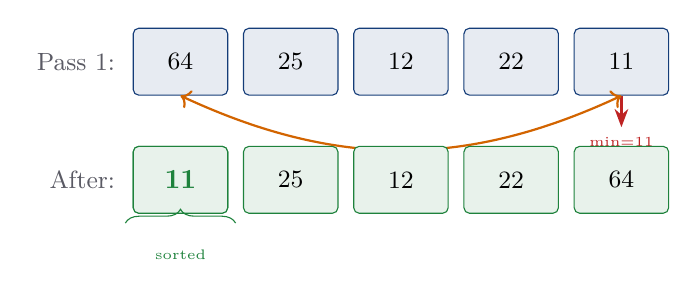
\begin{tikzpicture}[font=\small, every node/.style={rounded corners=2pt}]
  \foreach \v/\i in {64/0,25/1,12/2,22/3,11/4}{
    \node[draw=myblue,fill=myblue!10,minimum width=1.2cm,minimum height=0.85cm]
      (a\i) at (\i*1.4,1.5){\v};
  }
  \node[left=0.1cm of a0,text=mygray,font=\small]{Pass 1:};
  \draw[myred,-{Stealth},thick](a4.south)--++(0,-0.4)
    node[below,text=myred,font=\tiny]{min=11};
  \draw[myorange,<->,thick,bend right=25](a0.south) to
    node[below,font=\tiny,myorange]{swap}(a4.south);

  \foreach \v/\i in {11/0,25/1,12/2,22/3,64/4}{
    \node[draw=mygreen,fill=mygreen!10,minimum width=1.2cm,minimum height=0.85cm]
      (b\i) at (\i*1.4,0){\v};
  }
  \node[left=0.1cm of b0,text=mygray,font=\small]{After:};
  \node[draw=mygreen,fill=mygreen!10,text=mygreen,font=\bfseries,
        minimum width=1.2cm,minimum height=0.85cm](b0fixed) at (0,0){11};
  \draw[mygreen,decorate,decoration={brace,amplitude=5pt}]
    (-0.7,-0.55)--(0.7,-0.55)
    node[midway,below=6pt,font=\tiny,text=mygreen]{sorted};
\end{tikzpicture}
\end{center}

\begin{lstlisting}[caption={Selection Sort}]
public class SelectionSort {
    public static void selectionSort(int[] arr) {
        int n = arr.length;

        for (int i = 0; i < n - 1; i++) {
            // Find the index of the minimum element in arr[i..n-1]
            int minIndex = i;
            for (int j = i + 1; j < n; j++) {
                if (arr[j] < arr[minIndex]) {
                    minIndex = j;   // found a smaller element
                }
            }
            // Swap the minimum element to position i
            int temp        = arr[minIndex];
            arr[minIndex]   = arr[i];
            arr[i]          = temp;
        }
    }

    public static void main(String[] args) {
        int[] arr = {64, 25, 12, 22, 11};
        selectionSort(arr);
        for (int x : arr) System.out.print(x + " ");
        // Output: 11 12 22 25 64
    }
}
\end{lstlisting}

\begin{dryrun}[Dry Run: arr = \{64, 25, 12, 22, 11\}]
\begin{center}
\begin{tabular}{clll}
\toprule
\textbf{Pass (i)} & \textbf{Unsorted Region} & \textbf{Minimum Found} & \textbf{Array After Swap}\\
\midrule
0 & \{64,25,12,22,11\} & 11 at index 4 & \{11,25,12,22,64\}\\
1 & \{25,12,22,64\}    & 12 at index 2 & \{11,12,25,22,64\}\\
2 & \{25,22,64\}       & 22 at index 3 & \{11,12,22,25,64\}\\
3 & \{25,64\}          & 25 at index 3 & \{11,12,22,25,64\}\\
\bottomrule
\end{tabular}
\end{center}
\textbf{Result: \{11, 12, 22, 25, 64\}}
\end{dryrun}

\begin{complexity}
Time: $O(n^2)$ always (even if already sorted --- it still scans)\quad Space: $O(1)$\quad Stable: No
\end{complexity}

\section{Bubble Sort}

\textbf{Idea:} Repeatedly compare adjacent elements and swap if out of order. After each pass, the largest unsorted element ``bubbles'' to its correct position at the end.

\begin{lstlisting}[caption={Bubble Sort with early-exit optimisation}]
public class BubbleSort {
    public static void bubbleSort(int[] arr) {
        int n = arr.length;

        for (int i = 0; i < n - 1; i++) {
            boolean swapped = false;   // optimisation: detect already-sorted array

            // Inner loop: push the largest in arr[0..n-i-1] to its final position
            for (int j = 0; j < n - i - 1; j++) {
                if (arr[j] > arr[j + 1]) {
                    // Swap adjacent elements
                    int temp    = arr[j];
                    arr[j]      = arr[j + 1];
                    arr[j + 1]  = temp;
                    swapped = true;
                }
            }
            // If no swap happened in this pass, array is already sorted
            if (!swapped) break;
        }
    }

    public static void main(String[] args) {
        int[] arr = {5, 1, 4, 2, 8};
        bubbleSort(arr);
        for (int x : arr) System.out.print(x + " ");
        // Output: 1 2 4 5 8
    }
}
\end{lstlisting}

\begin{dryrun}[Dry Run: arr = \{5, 1, 4, 2, 8\}]
\begin{center}
\begin{tabular}{clll}
\toprule
\textbf{Pass (i)} & \textbf{Array Before} & \textbf{Comparisons \& Swaps} & \textbf{Array After}\\
\midrule
0 & \{5,1,4,2,8\} & 5$>$1 swap; 5$>$4 swap; 5$>$2 swap; 5$<$8 ok & \{1,4,2,5,8\}\\
1 & \{1,4,2,5,8\} & 1$<$4 ok; 4$>$2 swap; 4$<$5 ok               & \{1,2,4,5,8\}\\
2 & \{1,2,4,5,8\} & 1$<$2 ok; 2$<$4 ok  (no swaps)               & \{1,2,4,5,8\}\\
\multicolumn{4}{l}{swapped=false in pass 2 $\to$ \textbf{early exit!}}\\
\bottomrule
\end{tabular}
\end{center}
\textbf{Result: \{1, 2, 4, 5, 8\}}
\end{dryrun}

\begin{complexity}
Best: $O(n)$ (sorted input, early exit)\quad Worst/Average: $O(n^2)$\quad Space: $O(1)$\quad Stable: Yes
\end{complexity}

\section{Insertion Sort}

\textbf{Idea:} Build a sorted region from left to right. For each new element, insert it into its correct position in the sorted region --- just like sorting playing cards in your hand.

\begin{lstlisting}[caption={Insertion Sort}]
public class InsertionSort {
    public static void insertionSort(int[] arr) {
        int n = arr.length;

        for (int i = 1; i < n; i++) {
            int key = arr[i];   // the element to insert into sorted region
            int j   = i - 1;   // start of the sorted region's right end

            // Shift all sorted elements greater than key one position right
            while (j >= 0 && arr[j] > key) {
                arr[j + 1] = arr[j];
                j--;
            }
            // Place key at the correct position
            arr[j + 1] = key;
        }
    }

    public static void main(String[] args) {
        int[] arr = {12, 11, 13, 5, 6};
        insertionSort(arr);
        for (int x : arr) System.out.print(x + " ");
        // Output: 5 6 11 12 13
    }
}
\end{lstlisting}

\begin{dryrun}[Dry Run: arr = \{12, 11, 13, 5, 6\}]
\begin{center}
\begin{tabular}{clll}
\toprule
\textbf{i} & \textbf{key} & \textbf{Shifting} & \textbf{Array After Insert}\\
\midrule
1 & 11 & 12 $>$ 11: shift 12 right         & \{11, 12, 13, 5, 6\}\\
2 & 13 & 12 $\not>$ 13: no shift           & \{11, 12, 13, 5, 6\}\\
3 & 5  & 13,12,11 all $>$ 5: shift all     & \{5, 11, 12, 13, 6\}\\
4 & 6  & 13,12,11 $>$ 6: shift; 5 $<$ 6: stop & \{5, 6, 11, 12, 13\}\\
\bottomrule
\end{tabular}
\end{center}
\textbf{Result: \{5, 6, 11, 12, 13\}}
\end{dryrun}

\begin{complexity}
Best: $O(n)$ (already sorted)\quad Worst/Average: $O(n^2)$\quad Space: $O(1)$\quad Stable: Yes\\[4pt]
\textbf{Insertion Sort is preferred for small arrays ($n \leq 20$)} and nearly-sorted data.
\end{complexity}

\section{Merge Sort}

\textbf{Idea:} Divide and Conquer. Recursively split the array into halves until size 1, then \textit{merge} the sorted halves back together.

\begin{lstlisting}[caption={Merge Sort --- stable O(n log n) guaranteed}]
public class MergeSort {
    // Merge two sorted halves: arr[left..mid] and arr[mid+1..right]
    static void merge(int[] arr, int left, int mid, int right) {
        int n1 = mid - left + 1;
        int n2 = right - mid;

        int[] L = new int[n1];   // temp left half
        int[] R = new int[n2];   // temp right half

        for (int i = 0; i < n1; i++) L[i] = arr[left + i];
        for (int j = 0; j < n2; j++) R[j] = arr[mid + 1 + j];

        int i = 0, j = 0, k = left;
        while (i < n1 && j < n2) {
            if (L[i] <= R[j]) arr[k++] = L[i++];
            else               arr[k++] = R[j++];
        }
        while (i < n1) arr[k++] = L[i++];  // copy remaining left
        while (j < n2) arr[k++] = R[j++];  // copy remaining right
    }

    static void mergeSort(int[] arr, int left, int right) {
        if (left < right) {
            int mid = (left + right) / 2;
            mergeSort(arr, left, mid);        // sort left half
            mergeSort(arr, mid + 1, right);   // sort right half
            merge(arr, left, mid, right);     // merge sorted halves
        }
    }

    public static void main(String[] args) {
        int[] arr = {38, 27, 43, 3, 9, 82, 10};
        mergeSort(arr, 0, arr.length - 1);
        for (int x : arr) System.out.print(x + " ");
        // Output: 3 9 10 27 38 43 82
    }
}
\end{lstlisting}

\begin{dryrun}[Dry Run: arr = \{38, 27, 43, 3\}]
\begin{center}
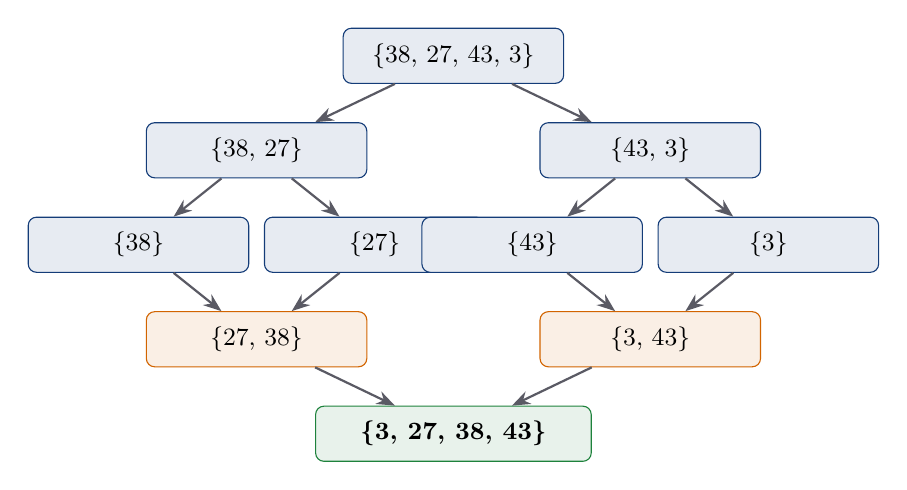
\begin{tikzpicture}[
  node/.style={draw=myblue,fill=myblue!10,rounded corners=3pt,
               font=\small,minimum width=2.8cm,minimum height=0.7cm,
               align=center},
  arr/.style={-{Stealth},thick,mygray}]
  \node[node](root) at (4,3) {\{38, 27, 43, 3\}};
  \node[node](l) at (1.5,1.8) {\{38, 27\}};
  \node[node](r) at (6.5,1.8) {\{43, 3\}};
  \node[node](ll) at (0,0.6) {\{38\}};
  \node[node](lr) at (3,0.6) {\{27\}};
  \node[node](rl) at (5,0.6) {\{43\}};
  \node[node](rr) at (8,0.6) {\{3\}};
  \draw[arr](root)--(l); \draw[arr](root)--(r);
  \draw[arr](l)--(ll); \draw[arr](l)--(lr);
  \draw[arr](r)--(rl); \draw[arr](r)--(rr);
  % merge back
  \node[draw=myorange,fill=myorange!10,rounded corners=3pt,font=\small,
        minimum width=2.8cm,minimum height=0.7cm,align=center]
    (ml) at (1.5,-0.6){\{27, 38\}};
  \node[draw=myorange,fill=myorange!10,rounded corners=3pt,font=\small,
        minimum width=2.8cm,minimum height=0.7cm,align=center]
    (mr) at (6.5,-0.6){\{3, 43\}};
  \node[draw=mygreen,fill=mygreen!10,rounded corners=3pt,font=\small\bfseries,
        minimum width=3.5cm,minimum height=0.7cm,align=center]
    (mfinal) at (4,-1.8){\{3, 27, 38, 43\}};
  \draw[myorange,arr](ll)--(ml); \draw[myorange,arr](lr)--(ml);
  \draw[myorange,arr](rl)--(mr); \draw[myorange,arr](rr)--(mr);
  \draw[mygreen,arr](ml)--(mfinal); \draw[mygreen,arr](mr)--(mfinal);
\end{tikzpicture}
\end{center}
\end{dryrun}

\begin{complexity}
Time: $O(n \log n)$ in all cases (best, average, worst)\quad Space: $O(n)$ auxiliary\quad Stable: Yes\\[4pt]
Preferred for sorting \textbf{Linked Lists}. Best choice when stability is required on large data.
\end{complexity}

\section{Quick Sort}

\textbf{Idea:} Choose a \textbf{pivot} element. Partition the array so all elements $<$ pivot go left and all $>$ pivot go right. Recursively sort both sides.

\begin{lstlisting}[caption={Quick Sort --- in-place, average O(n log n)}]
public class QuickSort {
    // Partition: place pivot at its correct sorted position
    static int partition(int[] arr, int low, int high) {
        int pivot = arr[high];   // choose last element as pivot
        int i     = low - 1;     // i tracks boundary of smaller elements

        for (int j = low; j < high; j++) {
            if (arr[j] <= pivot) {
                i++;
                // Swap arr[i] and arr[j]
                int temp = arr[i]; arr[i] = arr[j]; arr[j] = temp;
            }
        }
        // Place pivot in its correct position
        int temp = arr[i + 1]; arr[i + 1] = arr[high]; arr[high] = temp;
        return i + 1;   // return pivot's final index
    }

    static void quickSort(int[] arr, int low, int high) {
        if (low < high) {
            int pivotIndex = partition(arr, low, high);  // pivot is placed correctly
            quickSort(arr, low, pivotIndex - 1);          // sort left of pivot
            quickSort(arr, pivotIndex + 1, high);         // sort right of pivot
        }
    }

    public static void main(String[] args) {
        int[] arr = {10, 7, 8, 9, 1, 5};
        quickSort(arr, 0, arr.length - 1);
        for (int x : arr) System.out.print(x + " ");
        // Output: 1 5 7 8 9 10
    }
}
\end{lstlisting}

\begin{dryrun}[Dry Run: Partition on \{10, 7, 8, 9, 1, 5\}, pivot = 5]
\begin{center}
\begin{tabular}{ccccl}
\toprule
\textbf{j} & \textbf{arr[j]} & \textbf{arr[j] $\leq$ 5?} & \textbf{i} & \textbf{Action}\\
\midrule
0 & 10 & No  & -1 & skip\\
1 & 7  & No  & -1 & skip\\
2 & 8  & No  & -1 & skip\\
3 & 9  & No  & -1 & skip\\
4 & 1  & Yes & 0  & swap arr[0] $\leftrightarrow$ arr[4] $\to$ \{1,7,8,9,10,5\}\\
\multicolumn{5}{l}{End of loop: swap arr[i+1]=arr[1] with pivot arr[5]=5 $\to$ \{1,5,8,9,10,7\}}\\
\multicolumn{5}{l}{Pivot 5 is at index 1. Left \{1\}, Right \{8,9,10,7\} sorted recursively.}\\
\bottomrule
\end{tabular}
\end{center}
\end{dryrun}

\begin{complexity}
Best/Average: $O(n \log n)$\quad Worst: $O(n^2)$ (sorted array with last-element pivot)\quad Space: $O(\log n)$ call stack\quad Stable: No\\[4pt]
\textbf{In practice, Quick Sort is the fastest in-memory sort} due to excellent cache performance. Use randomised pivot to avoid $O(n^2)$ worst case.
\end{complexity}

\begin{interviewcorner}
\begin{itemize}
  \item ``Why is Quick Sort preferred over Merge Sort in practice?'' --- Better cache locality; in-place ($O(1)$ extra space vs $O(n)$)
  \item ``What is the worst case?'' --- Already sorted / reverse sorted array with fixed pivot
  \item ``How do you avoid worst case?'' --- Random pivot selection; or use median-of-three
  \item Quick Sort is \textbf{not stable}. If stability needed, use Merge Sort
\end{itemize}
\end{interviewcorner}

%%------------------------------------------------------------
\section{Heap Sort}
%%------------------------------------------------------------

\textbf{Idea:} Build a \textbf{Max-Heap} from the array. The largest element is always at the root (index 0). Swap it to the end, shrink the heap by one, and \textit{heapify} to restore the heap property. Repeat until sorted.

\textbf{Key concept --- heapify:} Given a node at index \texttt{i} in an array of size \texttt{n}, its children are at \texttt{2*i+1} (left) and \texttt{2*i+2} (right). Heapify pushes \texttt{arr[i]} down until it is larger than both children.

\begin{lstlisting}[caption={Heap Sort --- in-place O(n log n), not stable}]
public class HeapSort {

    // heapify: fix the heap rooted at index i, heap size = n
    static void heapify(int[] arr, int n, int i) {
        int largest = i;          // assume root is largest
        int left    = 2 * i + 1; // left child index
        int right   = 2 * i + 2; // right child index

        // if left child exists and is larger than root
        if (left < n && arr[left] > arr[largest])
            largest = left;

        // if right child exists and is larger than current largest
        if (right < n && arr[right] > arr[largest])
            largest = right;

        // if root is not the largest, swap and continue heapifying
        if (largest != i) {
            int temp    = arr[i];
            arr[i]      = arr[largest];
            arr[largest] = temp;

            heapify(arr, n, largest); // fix the affected subtree
        }
    }

    static void heapSort(int[] arr) {
        int n = arr.length;

        // Step 1: Build max-heap from the array
        // Start from last non-leaf node and heapify each node upward
        for (int i = n / 2 - 1; i >= 0; i--)
            heapify(arr, n, i);

        // Step 2: Extract elements one by one from heap
        for (int i = n - 1; i > 0; i--) {
            // Move current root (largest) to end
            int temp = arr[0];
            arr[0]   = arr[i];
            arr[i]   = temp;

            // Heapify the reduced heap (ignore sorted tail)
            heapify(arr, i, 0);
        }
    }

    public static void main(String[] args) {
        int[] arr = {12, 11, 13, 5, 6, 7};
        heapSort(arr);
        for (int x : arr) System.out.print(x + " ");
        // Output: 5 6 7 11 12 13
    }
}
\end{lstlisting}

\begin{dryrun}[Dry Run: arr = \{4, 10, 3, 5, 1\}]
\textbf{Step 1 — Build Max-Heap} (heapify from index 1 down to 0):

\begin{center}
\begin{tabular}{cl}
\toprule
\textbf{Heapify at i} & \textbf{Array after}\\
\midrule
$i=1$ & \{4, 10, 3, 5, 1\} \quad (10 $>$ 4, swap $\to$ no, 10 already largest child)\\
$i=0$ & \{10, 5, 3, 4, 1\} \quad (10 $>$ 4,5; swap root with 10; then fix subtree)\\
\bottomrule
\end{tabular}
\end{center}

\textbf{Step 2 — Extract max repeatedly:}

\begin{center}
\begin{tabular}{clll}
\toprule
\textbf{Pass} & \textbf{Swap (root $\leftrightarrow$ end)} & \textbf{Array} & \textbf{Sorted tail}\\
\midrule
1 & arr[0] $\leftrightarrow$ arr[4] & \{1,5,3,4,\textbf{10}\} & 10\\
  & heapify(4,0) & \{5,4,3,1,\textbf{10}\} & \\
2 & arr[0] $\leftrightarrow$ arr[3] & \{1,4,3,\textbf{5,10}\} & 5,10\\
  & heapify(3,0) & \{4,1,3,\textbf{5,10}\} & \\
3 & arr[0] $\leftrightarrow$ arr[2] & \{3,1,\textbf{4,5,10}\} & 4,5,10\\
  & heapify(2,0) & \{3,1,\textbf{4,5,10}\} & \\
4 & arr[0] $\leftrightarrow$ arr[1] & \{1,\textbf{3,4,5,10}\} & 3,4,5,10\\
\midrule
\multicolumn{4}{l}{Result: \{1, 3, 4, 5, 10\}}\\
\bottomrule
\end{tabular}
\end{center}
\end{dryrun}

\begin{complexity}
Time: $O(n \log n)$ best, average and worst\quad Space: $O(1)$ — fully in-place\quad Stable: No\\[4pt]
Best when memory is constrained. The $O(\log n)$ heapify runs $n$ times for build and $n$ times for extraction.
\end{complexity}

\begin{interviewcorner}
\begin{itemize}
  \item \textbf{Why not used in practice despite $O(n \log n)$?} --- Poor cache locality; heap accesses jump around in memory, unlike Quick Sort which accesses nearby indices
  \item \textbf{When is it preferred?} --- When guaranteed $O(n \log n)$ AND $O(1)$ space are both required
  \item \textbf{Is Heap Sort stable?} --- No. Equal elements may swap during heapify
  \item \textbf{What is a heap?} --- A complete binary tree stored as an array where every parent $\geq$ both children (max-heap)
\end{itemize}
\end{interviewcorner}

%%------------------------------------------------------------
\section{Radix Sort}
%%------------------------------------------------------------

\textbf{Idea:} Sort integers digit by digit, from the \textbf{least significant digit (LSD)} to the most significant digit. Use a \textbf{stable sort} (Counting Sort) at each digit pass. Since each pass is $O(n)$, and there are $d$ digit passes, total time is $O(d \cdot n)$.

\textbf{Key insight:} Radix Sort does \textit{not} compare elements. It distributes them into buckets 0--9 based on the current digit, then collects them in order.

\begin{lstlisting}[caption={Radix Sort --- O(d*n) time, O(n+b) space, stable}]
public class RadixSort {

    // Counting Sort on a specific digit position (exp = 1, 10, 100, ...)
    static void countingSort(int[] arr, int exp) {
        int n = arr.length;
        int[] output = new int[n];  // sorted output for this pass
        int[] count  = new int[10]; // buckets 0 to 9

        // Count how many numbers have digit d at position exp
        for (int i = 0; i < n; i++) {
            int digit = (arr[i] / exp) % 10;
            count[digit]++;
        }

        // Convert count[] to cumulative: count[i] now holds
        // the position of digit i in the output
        for (int i = 1; i < 10; i++)
            count[i] += count[i - 1];

        // Build output array (traverse right to left for stability)
        for (int i = n - 1; i >= 0; i--) {
            int digit = (arr[i] / exp) % 10;
            output[count[digit] - 1] = arr[i];
            count[digit]--;
        }

        // Copy output back into arr
        for (int i = 0; i < n; i++)
            arr[i] = output[i];
    }

    static void radixSort(int[] arr) {
        // Find maximum element to know number of digits
        int max = arr[0];
        for (int x : arr) if (x > max) max = x;

        // Do one counting sort pass for each digit position
        // exp = 1 (units), 10 (tens), 100 (hundreds), ...
        for (int exp = 1; max / exp > 0; exp *= 10)
            countingSort(arr, exp);
    }

    public static void main(String[] args) {
        int[] arr = {170, 45, 75, 90, 802, 24, 2, 66};
        radixSort(arr);
        for (int x : arr) System.out.print(x + " ");
        // Output: 2 24 45 66 75 90 170 802
    }
}
\end{lstlisting}

\begin{dryrun}[Dry Run: arr = \{170, 45, 75, 90, 802, 24, 2, 66\}]
Max = 802 $\to$ 3 digit passes needed.

\begin{center}
\begin{tabular}{cll}
\toprule
\textbf{Pass} & \textbf{Sort by digit} & \textbf{Array after pass}\\
\midrule
1 & Units (exp=1) & \{170, 90, 802, 2, 24, 45, 75, 66\}\\
2 & Tens (exp=10) & \{802, 2, 24, 45, 66, 170, 75, 90\}\\
3 & Hundreds (exp=100) & \{2, 24, 45, 66, 75, 90, 170, 802\}\\
\bottomrule
\end{tabular}
\end{center}

\textbf{Pass 1 detail} (sort by units digit):
Numbers grouped by last digit:\\
bucket[0]: 170, 90 \quad bucket[2]: 802, 2 \quad bucket[4]: 24 \quad bucket[5]: 45 \quad bucket[5]: 75 \quad bucket[6]: 66\\
Collect in order $\to$ \{170, 90, 802, 2, 24, 45, 75, 66\}
\end{dryrun}

\begin{complexity}
Time: $O(d \times n)$ where $d$ = number of digits in max element\quad Space: $O(n + b)$ where $b$ = base (10)\quad Stable: Yes\\[4pt]
For fixed-width integers (e.g.\ 32-bit), $d$ is constant, making it effectively $O(n)$ --- faster than any comparison sort.
\end{complexity}

\begin{interviewcorner}
\begin{itemize}
  \item \textbf{Why can Radix Sort beat $O(n \log n)$?} --- It does not compare elements; it counts and places. Comparison sorts have a theoretical lower bound of $O(n \log n)$; non-comparison sorts can bypass this
  \item \textbf{When to use?} --- Large arrays of integers with a bounded number of digits (phone numbers, IDs, scores)
  \item \textbf{Can it sort negative numbers?} --- Not directly. Separate negatives, sort absolute values, reverse and negate, then merge with positives
  \item \textbf{Why traverse right to left in counting sort?} --- To maintain stability: elements with the same digit keep their original relative order
\end{itemize}
\end{interviewcorner}

%%------------------------------------------------------------
\section{Counting Sort}
%%------------------------------------------------------------

\textbf{Idea:} Instead of comparing elements, \textbf{count how many times each value appears}. Then use those counts to place every element directly at its correct position. Works only when the range of values $k$ is known and reasonably small.

\textbf{When to use:} Elements are non-negative integers in a known range $[0, k]$. Example: sort exam scores (0--100), sort ages (0--120), sort characters.

\begin{lstlisting}[caption={Counting Sort --- O(n + k) time and space, stable}]
public class CountingSort {

    static void countingSort(int[] arr) {
        int n = arr.length;

        // Step 1: Find the maximum value to know range of counts
        int max = arr[0];
        for (int x : arr) if (x > max) max = x;

        // Step 2: Create count array of size max+1, initialised to 0
        int[] count = new int[max + 1];

        // Step 3: Count occurrences of each element
        for (int x : arr)
            count[x]++;
        // count[i] = how many times value i appears in arr

        // Step 4: Convert to cumulative counts
        // count[i] now = number of elements <= i
        for (int i = 1; i <= max; i++)
            count[i] += count[i - 1];

        // Step 5: Build output array (traverse right to left for stability)
        int[] output = new int[n];
        for (int i = n - 1; i >= 0; i--) {
            output[count[arr[i]] - 1] = arr[i]; // place at correct position
            count[arr[i]]--;                     // decrement for duplicates
        }

        // Step 6: Copy output back to arr
        for (int i = 0; i < n; i++)
            arr[i] = output[i];
    }

    public static void main(String[] args) {
        int[] arr = {4, 2, 2, 8, 3, 3, 1};
        countingSort(arr);
        for (int x : arr) System.out.print(x + " ");
        // Output: 1 2 2 3 3 4 8
    }
}
\end{lstlisting}

\begin{dryrun}[Dry Run: arr = \{4, 2, 2, 8, 3, 3, 1\}, max = 8]
\textbf{Step 3 — Count occurrences:}
\begin{center}
\begin{tabular}{!{\color{black!30}\vrule}l!{\color{black!30}\vrule}ccccccccc!{\color{black!30}\vrule}}
\toprule
\textbf{Index (value)} & 0 & 1 & 2 & 3 & 4 & 5 & 6 & 7 & 8\\
\midrule
\textbf{count[]}       & 0 & 1 & 2 & 2 & 1 & 0 & 0 & 0 & 1\\
\bottomrule
\end{tabular}
\end{center}

\textbf{Step 4 — Cumulative counts:}
\begin{center}
\begin{tabular}{!{\color{black!30}\vrule}l!{\color{black!30}\vrule}ccccccccc!{\color{black!30}\vrule}}
\toprule
\textbf{Index} & 0 & 1 & 2 & 3 & 4 & 5 & 6 & 7 & 8\\
\midrule
\textbf{count[]} & 0 & 1 & 3 & 5 & 6 & 6 & 6 & 6 & 7\\
\bottomrule
\end{tabular}
\end{center}

\textbf{Step 5 — Place elements} (right to left, \texttt{arr = \{4,2,2,8,3,3,1\}}):
\begin{center}
\begin{tabular}{cccl}
\toprule
\textbf{i} & \textbf{arr[i]} & \textbf{count[arr[i]]} & \textbf{Placed at index}\\
\midrule
6 & 1 & 1 & output[0] = 1\\
5 & 3 & 5 & output[4] = 3\\
4 & 3 & 4 & output[3] = 3\\
3 & 8 & 7 & output[6] = 8\\
2 & 2 & 3 & output[2] = 2\\
1 & 2 & 2 & output[1] = 2\\
0 & 4 & 6 & output[5] = 4\\
\midrule
\multicolumn{4}{l}{Result: \{1, 2, 2, 3, 3, 4, 8\}}\\
\bottomrule
\end{tabular}
\end{center}
\end{dryrun}

\begin{complexity}
Time: $O(n + k)$ where $k$ = range of values (max element)\quad Space: $O(n + k)$ for count and output arrays\quad Stable: Yes\\[4pt]
When $k = O(n)$, this is effectively $O(n)$ --- the fastest possible sort. But if $k \gg n$ (e.g.\ sorting 10 numbers in range 0--10\,000\,000), it wastes huge memory.
\end{complexity}

\begin{interviewcorner}
\begin{itemize}
  \item \textbf{Why is it $O(n + k)$ and not $O(n)$?} --- Even if the array has 5 elements but max is 1000, you still initialise and scan 1001 buckets
  \item \textbf{Can it handle negative numbers?} --- Yes, with an offset. Find \texttt{min}, shift all values by \texttt{-min} so the range starts at 0, sort, then shift back
  \item \textbf{Can it handle floats?} --- No. Only works for integer keys
  \item \textbf{Relationship to Radix Sort?} --- Radix Sort uses Counting Sort internally as its per-digit stable sort. Understanding Counting Sort is the key to understanding Radix Sort
  \item \textbf{Why right-to-left in Step 5?} --- Ensures stability: duplicate values appear in their original relative order in the output
\end{itemize}
\end{interviewcorner}

%%------------------------------------------------------------
\section{Tim Sort}
%%------------------------------------------------------------

\textbf{Idea:} Tim Sort is a \textbf{hybrid sorting algorithm} that combines \textbf{Insertion Sort} (for small subarrays) and \textbf{Merge Sort} (for merging). It was designed by Tim Peters in 2002 for Python and is now used in Java's \texttt{Arrays.sort()} for objects and Python's built-in \texttt{sort()}.

\textbf{Key concept --- run:} Tim Sort divides the array into small chunks called \textit{runs} (typically 32--64 elements). Each run is sorted with Insertion Sort (which is extremely fast on small arrays). Sorted runs are then merged using a merge similar to Merge Sort.

\begin{definitionbox}[Why Tim Sort?]
Real-world data is \textbf{rarely random}. It often has naturally ordered subsequences (partially sorted regions). Tim Sort detects these natural runs and exploits them, making it much faster than pure Merge Sort or Quick Sort on real data.
\end{definitionbox}

\begin{lstlisting}[caption={Tim Sort --- simplified implementation showing core idea}]
public class TimSort {

    static final int RUN = 32; // size of each small run

    // Step 1: Insertion Sort for a small subarray arr[left..right]
    static void insertionSort(int[] arr, int left, int right) {
        for (int i = left + 1; i <= right; i++) {
            int key = arr[i];
            int j   = i - 1;
            while (j >= left && arr[j] > key) {
                arr[j + 1] = arr[j];
                j--;
            }
            arr[j + 1] = key;
        }
    }

    // Step 2: Merge two sorted runs arr[left..mid] and arr[mid+1..right]
    static void merge(int[] arr, int left, int mid, int right) {
        int len1 = mid - left + 1;
        int len2 = right - mid;

        int[] L = new int[len1];
        int[] R = new int[len2];

        for (int i = 0; i < len1; i++) L[i] = arr[left + i];
        for (int i = 0; i < len2; i++) R[i] = arr[mid + 1 + i];

        int i = 0, j = 0, k = left;
        while (i < len1 && j < len2) {
            if (L[i] <= R[j]) arr[k++] = L[i++]; // <= keeps it stable
            else               arr[k++] = R[j++];
        }
        while (i < len1) arr[k++] = L[i++];
        while (j < len2) arr[k++] = R[j++];
    }

    // Step 3: Full Tim Sort
    static void timSort(int[] arr) {
        int n = arr.length;

        // Sort each run of size RUN using Insertion Sort
        for (int i = 0; i < n; i += RUN)
            insertionSort(arr, i, Math.min(i + RUN - 1, n - 1));

        // Merge runs: start with size RUN, then 2*RUN, 4*RUN, ...
        for (int size = RUN; size < n; size *= 2) {
            for (int left = 0; left < n; left += 2 * size) {
                int mid   = Math.min(left + size - 1, n - 1);
                int right = Math.min(left + 2 * size - 1, n - 1);

                if (mid < right) // only merge if there is a right run
                    merge(arr, left, mid, right);
            }
        }
    }

    public static void main(String[] args) {
        int[] arr = {5, 21, 7, 23, 19, 2, 11, 3, 8, 14};
        timSort(arr);
        for (int x : arr) System.out.print(x + " ");
        // Output: 2 3 5 7 8 11 14 19 21 23
    }
}
\end{lstlisting}

\begin{dryrun}[Dry Run concept: arr = \{5, 21, 7, 23, 19, 2, 11, 3, 8, 14\}, RUN = 4]
\begin{center}
\begin{tabular}{cl}
\toprule
\textbf{Phase} & \textbf{What happens}\\
\midrule
\textbf{Split into runs} & Run 1: \{5,21,7,23\} \quad Run 2: \{19,2,11,3\} \quad Run 3: \{8,14\}\\
\textbf{Insertion Sort each run} & Run 1 $\to$ \{5,7,21,23\}\\
  & Run 2 $\to$ \{2,3,11,19\}\\
  & Run 3 $\to$ \{8,14\} (already sorted)\\
\textbf{Merge pass 1 (size=4)} & Merge Run1 + Run2 $\to$ \{2,3,5,7,11,19,21,23\}\\
\textbf{Merge pass 2 (size=8)} & Merge result + Run3 $\to$ \{2,3,5,7,8,11,14,19,21,23\}\\
\bottomrule
\end{tabular}
\end{center}
\end{dryrun}

\begin{complexity}
Time: $O(n \log n)$ worst case\quad Best: $O(n)$ when array is already sorted (natural runs cover everything)\quad Space: $O(n)$ for merge\quad Stable: Yes\\[4pt]
In practice, Tim Sort outperforms pure Merge Sort and Quick Sort on real-world data because it exploits existing order. This is why Java and Python use it as their default sort.
\end{complexity}

\begin{interviewcorner}
\begin{itemize}
  \item \textbf{``What does \texttt{Arrays.sort()} use in Java?''} --- For primitive arrays (\texttt{int[]}, \texttt{double[]}) Java uses \textbf{Dual-Pivot Quick Sort}. For object arrays (\texttt{Integer[]}, \texttt{String[]}) Java uses \textbf{Tim Sort} because object sorting requires stability
  \item \textbf{Why Insertion Sort for small runs?} --- For $n \leq 32$, Insertion Sort's low overhead beats Merge Sort's recursive splitting cost. This crossover point is well-studied
  \item \textbf{What is a ``natural run''?} --- A maximal already-ascending (or descending) subsequence. Tim Sort detects these and avoids re-sorting them
  \item \textbf{Why is Tim Sort stable?} --- The \texttt{<=} in the merge step ensures equal elements from the left run come before those from the right run, preserving original order
  \item \textbf{Tim Sort vs Merge Sort?} --- Tim Sort is Merge Sort with two key optimisations: uses Insertion Sort for small chunks, and exploits pre-existing order in real data
\end{itemize}
\end{interviewcorner}

\section{Sorting Algorithms --- When to Use Which}
%%------------------------------------------------------------

\begin{center}
\renewcommand{\arraystretch}{1.55}
\setlength{\tabcolsep}{9pt}
\begin{tabular}{
  !{\color{myblue}\vrule width 1.2pt}
  >{\bfseries}p{5.2cm}
  !{\color{myblue!40}\vrule}
  p{2.8cm}
  !{\color{myblue!40}\vrule}
  p{5.8cm}
  !{\color{myblue}\vrule width 1.2pt}
}
% ---- header row ----
\arrayrulecolor{myblue}\hline
\rowcolor{myblue}
\color{white}\textbf{Situation} &
\color{white}\textbf{Best Choice} &
\color{white}\textbf{Why}\\
\arrayrulecolor{myblue}\hline
% ---- body rows, alternating shading ----
\rowcolor{myblue!8}
Small array ($n \leq 20$)        & Insertion Sort & Low overhead; nearly $O(n)$ if nearly sorted\\
\rowcolor{white}
General purpose, in-place        & Quick Sort     & Best average cache performance\\
\rowcolor{myblue!8}
Stability required               & Merge Sort     & Stable; $O(n \log n)$ guaranteed\\
\rowcolor{white}
Guaranteed $O(n \log n)$ + $O(1)$ space & Heap Sort & No $O(n^2)$ worst case, no extra memory\\
\rowcolor{myblue!8}
Large integer arrays             & Radix Sort     & Effectively $O(n)$ for bounded digit count\\
\rowcolor{white}
Small range integers             & Counting Sort  & $O(n + k)$ --- fastest when range $k$ is small\\
\rowcolor{myblue!8}
Real-world Java / Python sort    & Tim Sort       & What \texttt{Arrays.sort()} actually uses internally\\
\rowcolor{white}
Linked List sorting              & Merge Sort     & No random access needed\\
\rowcolor{myblue!8}
Nearly sorted data               & Insertion Sort & Best case $O(n)$\\
\arrayrulecolor{myblue}\hline
\end{tabular}
\end{center}

%%############################################################
\chapter{ArrayList}
%%############################################################

An \textbf{ArrayList} is a resizable array from \texttt{java.util}. Unlike a plain array, its size grows and shrinks automatically. Internally it uses an array; when that array is full, Java creates a new one roughly 1.5× larger and copies everything across.

\begin{definitionbox}{ArrayList vs Array}
\begin{center}
\begin{tabular}{p{3.5cm}p{3.8cm}p{4.5cm}}
\toprule
\textbf{Feature} & \textbf{Array} & \textbf{ArrayList}\\
\midrule
Size        & Fixed at creation     & Dynamic (grows/shrinks)\\
Type        & Primitives allowed    & Objects only (wrappers)\\
Syntax      & \texttt{int[] a}      & \texttt{ArrayList<Integer>}\\
Import      & None                  & \texttt{java.util.ArrayList}\\
Length      & \texttt{a.length}     & \texttt{a.size()}\\
Access      & \texttt{a[i]}         & \texttt{a.get(i)}\\
Set         & \texttt{a[i] = v}     & \texttt{a.set(i, v)}\\
Add element & Not possible          & \texttt{a.add(v)}\\
Remove      & Not possible          & \texttt{a.remove(i)}\\
\bottomrule
\end{tabular}
\end{center}
\end{definitionbox}

%%------------------------------------------------------------
\section{Creating an ArrayList}
%%------------------------------------------------------------

\begin{lstlisting}[caption={ArrayList --- Declaration and Initialisation}]
import java.util.ArrayList;

public class ArrayListBasics {
    public static void main(String[] args) {

        // 1. Empty ArrayList of integers
        ArrayList<Integer> nums = new ArrayList<>();

        // 2. ArrayList with initial capacity hint (does NOT set size)
        ArrayList<Integer> big = new ArrayList<>(100);

        // 3. Pre-filled using add()
        ArrayList<String> names = new ArrayList<>();
        names.add("Alice");
        names.add("Bob");
        names.add("Charlie");

        System.out.println(names);        // [Alice, Bob, Charlie]
        System.out.println(names.size()); // 3
    }
}
\end{lstlisting}

\begin{tipbox}[Wrapper Classes]
ArrayList cannot store primitives directly. Use wrapper classes:\\
\texttt{int} $\to$ \texttt{Integer}, \quad \texttt{double} $\to$ \texttt{Double}, \quad \texttt{char} $\to$ \texttt{Character}, \quad \texttt{boolean} $\to$ \texttt{Boolean}\\
Java auto-boxes and unboxes automatically: \texttt{nums.add(5)} works even though 5 is a primitive.
\end{tipbox}

%%------------------------------------------------------------
\section{Common Operations}
%%------------------------------------------------------------

\begin{lstlisting}[caption={ArrayList --- All Core Operations}]
import java.util.ArrayList;
import java.util.Collections;

public class ArrayListOps {
    public static void main(String[] args) {

        ArrayList<Integer> list = new ArrayList<>();

        // ── ADD ──────────────────────────────────────────
        list.add(10);          // append to end      -> [10]
        list.add(20);          //                    -> [10, 20]
        list.add(30);          //                    -> [10, 20, 30]
        list.add(1, 99);       // insert at index 1  -> [10, 99, 20, 30]

        // ── ACCESS ───────────────────────────────────────
        int first = list.get(0);          // 10
        int last  = list.get(list.size() - 1); // 30

        // ── UPDATE ───────────────────────────────────────
        list.set(1, 55);       // replace index 1    -> [10, 55, 20, 30]

        // ── REMOVE ───────────────────────────────────────
        list.remove(2);        // remove by index    -> [10, 55, 30]
        list.remove(Integer.valueOf(55)); // remove by value -> [10, 30]

        // ── SEARCH ───────────────────────────────────────
        boolean has = list.contains(30); // true
        int idx     = list.indexOf(30);  // 1

        // ── SIZE & EMPTY ─────────────────────────────────
        int sz   = list.size();      // 2
        boolean e = list.isEmpty();  // false

        // ── SORT & REVERSE ───────────────────────────────
        list.add(5); list.add(40); list.add(1);
        Collections.sort(list);           // [1, 5, 10, 30, 40]
        Collections.reverse(list);        // [40, 30, 10, 5, 1]
        Collections.sort(list, Collections.reverseOrder()); // descending

        // ── CLEAR ────────────────────────────────────────
        list.clear();          // []
        System.out.println(list.isEmpty()); // true
    }
}
\end{lstlisting}

%%------------------------------------------------------------
\section{Traversal Methods}
%%------------------------------------------------------------

\begin{lstlisting}[caption={ArrayList --- Four Ways to Traverse}]
import java.util.ArrayList;

public class Traverse {
    public static void main(String[] args) {

        ArrayList<Integer> list = new ArrayList<>();
        for (int i = 1; i <= 5; i++) list.add(i * 10);
        // list = [10, 20, 30, 40, 50]

        // 1. Traditional for loop (when index needed)
        for (int i = 0; i < list.size(); i++) {
            System.out.print(list.get(i) + " ");
        }

        // 2. Enhanced for-each (simplest, read-only)
        for (int x : list) {
            System.out.print(x + " ");
        }

        // 3. While loop
        int i = 0;
        while (i < list.size()) {
            System.out.print(list.get(i) + " ");
            i++;
        }

        // 4. forEach with lambda (Java 8+)
        list.forEach(x -> System.out.print(x + " "));
    }
}
\end{lstlisting}

%%------------------------------------------------------------
\section{Size of an ArrayList}
%%------------------------------------------------------------

\textbf{Problem:} Print the size of an ArrayList before and after adding elements.

\begin{lstlisting}[caption={ArrayList --- size() demo}]
import java.util.ArrayList;

public class SizeDemo {
    public static void main(String[] args) {
        ArrayList<Integer> list = new ArrayList<>();
        System.out.println("Before: " + list.size()); // 0

        list.add(5);
        list.add(10);
        list.add(15);

        System.out.println("After:  " + list.size()); // 3

        list.remove(0);
        System.out.println("After remove: " + list.size()); // 2
    }
}
\end{lstlisting}

\begin{dryrun}[list starts empty]
\begin{center}
\begin{tabular}{clc}
\toprule
\textbf{Operation} & \textbf{list state} & \textbf{size()}\\
\midrule
initial           & \texttt{[]}          & 0\\
add(5)            & \texttt{[5]}         & 1\\
add(10)           & \texttt{[5, 10]}     & 2\\
add(15)           & \texttt{[5, 10, 15]} & 3\\
remove(0)         & \texttt{[10, 15]}    & 2\\
\bottomrule
\end{tabular}
\end{center}
\end{dryrun}

%%------------------------------------------------------------
\section{Print Reverse of an ArrayList}
%%------------------------------------------------------------

\textbf{Problem:} Print all elements of an ArrayList in reverse order without modifying it.

\begin{lstlisting}[caption={Print Reverse --- O(n) time O(1) extra space}]
import java.util.ArrayList;

public class PrintReverse {
    public static void printReverse(ArrayList<Integer> list) {
        // Start from last index, go down to 0
        for (int i = list.size() - 1; i >= 0; i--) {
            System.out.print(list.get(i) + " ");
        }
        System.out.println();
    }

    public static void main(String[] args) {
        ArrayList<Integer> list = new ArrayList<>();
        list.add(10); list.add(20); list.add(30); list.add(40); list.add(50);
        // Original: [10, 20, 30, 40, 50]
        printReverse(list); // Output: 50 40 30 20 10
    }
}
\end{lstlisting}

\begin{dryrun}[list = {[10, 20, 30, 40, 50]}]
\begin{center}
\begin{tabular}{ccl}
\toprule
\textbf{i} & \textbf{list.get(i)} & \textbf{printed}\\
\midrule
4 & 50 & 50\\
3 & 40 & 40\\
2 & 30 & 30\\
1 & 20 & 20\\
0 & 10 & 10\\
\bottomrule
\end{tabular}
\end{center}
\end{dryrun}

\begin{complexity}
Time: $O(n)$ --- one reverse pass\quad Space: $O(1)$ extra (no copy made)
\end{complexity}

%%------------------------------------------------------------
\section{Swap Two Numbers in an ArrayList}
%%------------------------------------------------------------

\textbf{Problem:} Swap elements at two given indices in an ArrayList.

\begin{lstlisting}[caption={Swap Two Numbers in ArrayList}]
import java.util.ArrayList;
import java.util.Collections;

public class SwapNumbers {
    public static void main(String[] args) {
        ArrayList<Integer> list = new ArrayList<>();
        list.add(10); list.add(20); list.add(30); list.add(40);

        int i = 1, j = 3; // swap index 1 and index 3

        // Method 1: Manual swap using set()
        int temp = list.get(i);
        list.set(i, list.get(j));
        list.set(j, temp);
        System.out.println(list); // [10, 40, 30, 20]

        // Method 2: Using Collections.swap() -- one-liner
        Collections.swap(list, 0, 2);
        System.out.println(list); // [30, 40, 10, 20]
    }
}
\end{lstlisting}

\begin{dryrun}[list = {[10, 20, 30, 40]}, swap i=1, j=3]
\begin{center}
\begin{tabular}{lll}
\toprule
\textbf{Step} & \textbf{Action} & \textbf{list}\\
\midrule
Initial  & ---                       & \texttt{[10, 20, 30, 40]}\\
temp=20  & \texttt{temp = get(1)}    & \texttt{[10, 20, 30, 40]}\\
set(1,40)& copy get(3) to index 1   & \texttt{[10, 40, 30, 40]}\\
set(3,20)& copy temp to index 3     & \texttt{[10, 40, 30, 20]}\\
\bottomrule
\end{tabular}
\end{center}
\end{dryrun}

\begin{complexity}
Time: $O(1)$\quad Space: $O(1)$
\end{complexity}

%%------------------------------------------------------------
\section{Find Maximum in an ArrayList}
%%------------------------------------------------------------

\textbf{Problem:} Find the largest element in an ArrayList.

\begin{lstlisting}[caption={Find Maximum --- Linear Scan}]
import java.util.ArrayList;
import java.util.Collections;

public class FindMax {
    public static int findMax(ArrayList<Integer> list) {
        int max = list.get(0);        // assume first is max
        for (int i = 1; i < list.size(); i++) {
            if (list.get(i) > max) {
                max = list.get(i);    // update whenever we find a bigger value
            }
        }
        return max;
    }

    public static void main(String[] args) {
        ArrayList<Integer> list = new ArrayList<>();
        list.add(3); list.add(7); list.add(1); list.add(9); list.add(4);

        System.out.println("Max: " + findMax(list));          // 9
        System.out.println("Max (API): " + Collections.max(list)); // 9
    }
}
\end{lstlisting}

\begin{dryrun}[list = {[3, 7, 1, 9, 4]}]
\begin{center}
\begin{tabular}{ccc}
\toprule
\textbf{i} & \textbf{list.get(i)} & \textbf{max}\\
\midrule
— & —  & 3 (initial)\\
1 & 7  & 7\\
2 & 1  & 7\\
3 & 9  & 9\\
4 & 4  & 9\\
\bottomrule
\end{tabular}
\end{center}
\end{dryrun}

\begin{complexity}
Time: $O(n)$\quad Space: $O(1)$
\end{complexity}

%%------------------------------------------------------------
\section{Sorting an ArrayList}
%%------------------------------------------------------------

\textbf{Problem:} Sort an ArrayList in ascending and descending order.

\begin{lstlisting}[caption={Sort ArrayList --- Ascending and Descending}]
import java.util.ArrayList;
import java.util.Collections;

public class SortArrayList {
    public static void main(String[] args) {
        ArrayList<Integer> list = new ArrayList<>();
        list.add(5); list.add(1); list.add(9); list.add(3); list.add(7);

        // Ascending (natural order)
        Collections.sort(list);
        System.out.println("Ascending:  " + list); // [1, 3, 5, 7, 9]

        // Descending (reverse order)
        Collections.sort(list, Collections.reverseOrder());
        System.out.println("Descending: " + list); // [9, 7, 5, 3, 1]
    }
}
\end{lstlisting}

\begin{tipbox}[Sorting Strings]
\texttt{Collections.sort()} also works on \texttt{ArrayList<String>} --- it sorts lexicographically (dictionary order).
\end{tipbox}

\begin{complexity}
Time: $O(n \log n)$ --- Tim Sort internally\quad Space: $O(n)$
\end{complexity}

%%------------------------------------------------------------
\section{Multi-Dimensional ArrayList}
%%------------------------------------------------------------

A 2-D ArrayList is an \texttt{ArrayList} of \texttt{ArrayList}s. Each inner list can have a different length, making it a \textbf{jagged} structure — unlike a 2-D array which is always rectangular.

\begin{lstlisting}[caption={2-D ArrayList --- Declare, Fill, and Print}]
import java.util.ArrayList;

public class MultiDim {
    public static void main(String[] args) {

        // A 2-D ArrayList (list of lists)
        ArrayList<ArrayList<Integer>> matrix = new ArrayList<>();

        // Add three rows of different lengths
        ArrayList<Integer> row0 = new ArrayList<>();
        row0.add(1); row0.add(2); row0.add(3);

        ArrayList<Integer> row1 = new ArrayList<>();
        row1.add(4); row1.add(5);

        ArrayList<Integer> row2 = new ArrayList<>();
        row2.add(6); row2.add(7); row2.add(8); row2.add(9);

        matrix.add(row0);
        matrix.add(row1);
        matrix.add(row2);

        // Print
        for (int i = 0; i < matrix.size(); i++) {
            for (int j = 0; j < matrix.get(i).size(); j++) {
                System.out.print(matrix.get(i).get(j) + " ");
            }
            System.out.println();
        }
        // Output:
        // 1 2 3
        // 4 5
        // 6 7 8 9
    }
}
\end{lstlisting}

\begin{center}
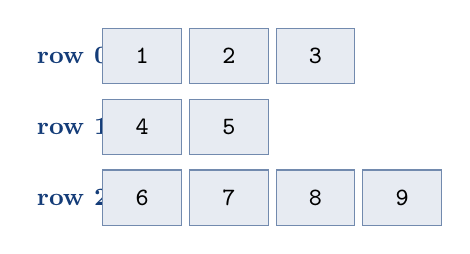
\begin{tikzpicture}[
  cell/.style={draw=myblue!60, fill=myblue!10, minimum width=1.0cm, minimum height=0.7cm, font=\ttfamily\small},
  rowlabel/.style={font=\small\bfseries\color{myblue}, anchor=east}
]
% Row 0
\node[rowlabel] at (-0.3, 0)    {row 0};
\foreach \v/\x in {1/0, 2/1, 3/2} {
  \node[cell] at (\x*1.1, 0) {\v};
}
% Row 1
\node[rowlabel] at (-0.3, -0.9) {row 1};
\foreach \v/\x in {4/0, 5/1} {
  \node[cell] at (\x*1.1, -0.9) {\v};
}
% Row 2
\node[rowlabel] at (-0.3, -1.8) {row 2};
\foreach \v/\x in {6/0, 7/1, 8/2, 9/3} {
  \node[cell] at (\x*1.1, -1.8) {\v};
}
\end{tikzpicture}
\end{center}

\begin{tipbox}[When to Use 2-D ArrayList vs 2-D Array]
Use \texttt{ArrayList<ArrayList<Integer>>} when rows have different lengths (Pascal's Triangle, adjacency list for graphs). Use \texttt{int[][]} when the grid is always rectangular and size is fixed.
\end{tipbox}

%%------------------------------------------------------------
\section{ArrayList --- Interview Corner}
%%------------------------------------------------------------

\begin{interviewcorner}[ArrayList --- Must-Know for Interviews]
\begin{itemize}
  \item \textbf{Time complexities:} \texttt{add()} amortized $O(1)$; \texttt{get(i)} $O(1)$; \texttt{remove(i)} $O(n)$ due to shifting; \texttt{contains()} $O(n)$
  \item \textbf{ArrayList vs LinkedList:} ArrayList gives $O(1)$ random access; LinkedList gives $O(1)$ insert/delete at ends. Use ArrayList for most cases.
  \item \textbf{ArrayList vs Array:} When size is unknown at compile time, use ArrayList. When primitives and performance are critical, use array.
  \item \textbf{Auto-boxing cost:} Every \texttt{add(int)} boxes the int to Integer --- negligible for small lists but relevant in hot loops.
  \item \textbf{ConcurrentModificationException:} Never add/remove inside a for-each loop. Use an explicit index loop or iterator's \texttt{remove()} instead.
  \item \textbf{Return type in problems:} Most LeetCode/interview problems return \texttt{List<Integer>} or \texttt{List<List<Integer>>} --- ArrayList is the standard concrete implementation.
  \item \textbf{Convert array $\leftrightarrow$ ArrayList:}
    \begin{itemize}
      \item Array to List: \texttt{Arrays.asList(arr)} (fixed size) or loop + \texttt{add()}
      \item List to Array: \texttt{list.toArray(new Integer[0])}
    \end{itemize}
\end{itemize}
\end{interviewcorner}

%%############################################################
%%------------------------------------------------------------
%%############################################################
\chapter{Array Problems --- Medium Level}
\index{Arrays!medium problems}
%%############################################################

\section{Sort 0s, 1s, and 2s --- Dutch National Flag}

\textbf{Problem:} Sort an array containing only 0, 1, and 2, \textit{in-place}, in one pass.

\begin{lstlisting}[caption={Dutch National Flag Algorithm --- O(n) time O(1) space}]
public class SortColors {
    public static void sort012(int[] arr) {
        int low  = 0;                 // everything before low is 0
        int mid  = 0;                 // current element under inspection
        int high = arr.length - 1;    // everything after high is 2

        while (mid <= high) {
            if (arr[mid] == 0) {
                // Swap arr[low] and arr[mid]; both 0-region and mid advance
                int t = arr[low]; arr[low] = arr[mid]; arr[mid] = t;
                low++;
                mid++;
            } else if (arr[mid] == 1) {
                mid++;        // 1 is in the correct middle region; just move on
            } else {          // arr[mid] == 2
                // Swap arr[mid] and arr[high]; only high retreats
                int t = arr[mid]; arr[mid] = arr[high]; arr[high] = t;
                high--;
                // DO NOT increment mid: element swapped from high is unchecked!
            }
        }
    }

    public static void main(String[] args) {
        int[] arr = {2, 0, 2, 1, 1, 0};
        sort012(arr);
        for (int x : arr) System.out.print(x + " ");
        // Output: 0 0 1 1 2 2
    }
}
\end{lstlisting}

\textbf{Three-region invariant maintained at all times:}

\begin{center}
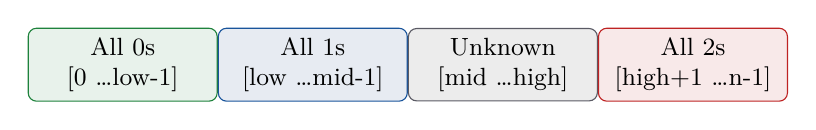
\begin{tikzpicture}[font=\small]
  \node[draw=mygreen, fill=mygreen!10, minimum width=2.4cm, minimum height=0.85cm,
        align=center, rounded corners=3pt](z) at (0,0){All 0s\\{[0 \ldots low-1]}};
  \node[draw=mybluelt, fill=myblue!10, minimum width=2.4cm, minimum height=0.85cm,
        align=center, rounded corners=3pt, right=0 of z](o){All 1s\\{[low \ldots mid-1]}};
  \node[draw=mygray, fill=gray!15, minimum width=2.4cm, minimum height=0.85cm,
        align=center, rounded corners=3pt, right=0 of o](u){Unknown\\{[mid \ldots high]}};
  \node[draw=myred, fill=myred!10, minimum width=2.4cm, minimum height=0.85cm,
        align=center, rounded corners=3pt, right=0 of u](t){All 2s\\{[high+1 \ldots n-1]}};
\end{tikzpicture}
\end{center}

\begin{dryrun}[Dry Run: arr = \{2, 0, 2, 1, 1, 0\}]
\begin{center}
\begin{tabular}{ccccll}
\toprule
\textbf{low} & \textbf{mid} & \textbf{high} & \textbf{arr[mid]} & \textbf{Array} & \textbf{Action}\\
\midrule
0 & 0 & 5 & 2 & \{2,0,2,1,1,0\} & swap(mid,high), high--\\
0 & 0 & 4 & 0 & \{0,0,2,1,1,2\} & swap(mid,low), low++,mid++\\
1 & 1 & 4 & 0 & \{0,0,2,1,1,2\} & swap(mid,low), low++,mid++\\
2 & 2 & 4 & 2 & \{0,0,2,1,1,2\} & swap(mid,high), high--\\
2 & 2 & 3 & 1 & \{0,0,1,1,2,2\} & mid++\\
2 & 3 & 3 & 1 & \{0,0,1,1,2,2\} & mid++\\
\multicolumn{6}{l}{mid(4) $>$ high(3): done. \textbf{Result: \{0,0,1,1,2,2\}}}\\
\bottomrule
\end{tabular}
\end{center}
\end{dryrun}

\begin{complexity}
Time: $O(n)$ --- single pass\quad Space: $O(1)$ --- in-place
\end{complexity}

\begin{interviewcorner}
Known as the \textbf{``Dutch National Flag Algorithm''}, invented by Edsger Dijkstra. Critical rule: when swapping \texttt{arr[mid]} with \texttt{arr[high]}, do \textbf{not} increment \texttt{mid} --- the element that came from \texttt{arr[high]} has never been inspected.
\end{interviewcorner}

\section{Majority Element --- Boyer-Moore Voting}

\textbf{Problem:} Find the element that appears \textbf{more than $n/2$ times}.

\begin{lstlisting}[caption={Boyer-Moore Voting Algorithm}]
public class MajorityElement {
    public static int majorityElement(int[] arr) {
        int candidate = arr[0];
        int count     = 1;

        // Phase 1: Find the candidate using vote cancellation
        for (int i = 1; i < arr.length; i++) {
            if (arr[i] == candidate) {
                count++;              // same element: vote for it
            } else {
                count--;              // different: cancel one vote
                if (count == 0) {
                    candidate = arr[i];  // candidate eliminated; pick new one
                    count = 1;
                }
            }
        }

        // Phase 2: Verify (necessary when majority not guaranteed to exist)
        int frequency = 0;
        for (int x : arr) {
            if (x == candidate) frequency++;
        }
        return (frequency > arr.length / 2) ? candidate : -1;
    }

    public static void main(String[] args) {
        int[] arr = {3, 2, 3, 1, 3, 4, 3};
        System.out.println(majorityElement(arr));  // 3
    }
}
\end{lstlisting}

\begin{dryrun}[Dry Run: arr = \{3, 2, 3, 1, 3, 4, 3\}]
\begin{center}
\begin{tabular}{cccl}
\toprule
\textbf{i} & \textbf{arr[i]} & \textbf{candidate / count} & \textbf{Note}\\
\midrule
0 & 3 & 3 / 1 & Initialise\\
1 & 2 & 3 / 0 & different: count-- $\to$ 0\\
2 & 3 & 3 / 1 & count=0, new candidate = 3\\
3 & 1 & 3 / 0 & different: count-- $\to$ 0\\
4 & 3 & 3 / 1 & new candidate = 3\\
5 & 4 & 3 / 0 & different: count-- $\to$ 0\\
6 & 3 & 3 / 1 & new candidate = 3\\
\bottomrule
\end{tabular}
\end{center}
\textbf{Verify:} 3 appears 4 times; $4 > 7/2 = 3$ \checkmark \quad \textbf{Result: 3}
\end{dryrun}

\begin{complexity}
Time: $O(n)$ two passes\quad Space: $O(1)$\quad (HashMap approach: $O(n)$ time + $O(n)$ space)
\end{complexity}

\section{Kadane's Algorithm --- Maximum Subarray Sum}

\textbf{Problem:} Find the contiguous subarray with the largest sum.

\textbf{Example:} arr = \{$-2, 1, -3, 4, -1, 2, 1, -5, 4$\} $\to$ answer = 6 (subarray \{4, $-1$, 2, 1\})

\begin{lstlisting}[caption={Kadane's Algorithm --- O(n) time O(1) space}]
public class KadanesAlgorithm {
    public static int maxSubarraySum(int[] arr) {
        int maxSum     = arr[0];   // best sum seen overall
        int currentSum = arr[0];   // best sum ending at current index

        for (int i = 1; i < arr.length; i++) {
            // Either extend the previous subarray OR start a fresh one
            currentSum = Math.max(arr[i], currentSum + arr[i]);
            maxSum     = Math.max(maxSum, currentSum);
        }
        return maxSum;
    }

    // BONUS: also return the subarray's start and end indices
    public static void maxSubarrayWithIndices(int[] arr) {
        int maxSum = arr[0], currentSum = arr[0];
        int start = 0, end = 0, tempStart = 0;

        for (int i = 1; i < arr.length; i++) {
            if (arr[i] > currentSum + arr[i]) {
                currentSum = arr[i];   // start fresh subarray
                tempStart  = i;
            } else {
                currentSum += arr[i];  // extend current subarray
            }
            if (currentSum > maxSum) {
                maxSum = currentSum;
                start  = tempStart;
                end    = i;
            }
        }
        System.out.println("Max Sum = " + maxSum);
        System.out.print("Subarray: ");
        for (int i = start; i <= end; i++) System.out.print(arr[i] + " ");
    }

    public static void main(String[] args) {
        int[] arr = {-2, 1, -3, 4, -1, 2, 1, -5, 4};
        System.out.println(maxSubarraySum(arr));   // 6
        maxSubarrayWithIndices(arr);               // Max Sum=6, Subarray: 4 -1 2 1
    }
}
\end{lstlisting}

\begin{dryrun}[Dry Run: arr = \{$-2$, 1, $-3$, 4, $-1$, 2, 1, $-5$, 4\}]
\begin{center}
\begin{tabular}{cccl}
\toprule
\textbf{i} & \textbf{arr[i]} & \textbf{currentSum} & \textbf{maxSum}\\
\midrule
init& ---& $-2$ & $-2$\\
1 & 1    & $\max(1,\ -2+1)=1$     & 1\\
2 & $-3$ & $\max(-3,\ 1-3)=-2$    & 1\\
3 & 4    & $\max(4,\ -2+4)=4$     & 4\\
4 & $-1$ & $\max(-1,\ 4-1)=3$     & 4\\
5 & 2    & $\max(2,\ 3+2)=5$      & 5\\
6 & 1    & $\max(1,\ 5+1)=6$      & \textbf{6}\\
7 & $-5$ & $\max(-5,\ 6-5)=1$     & 6\\
8 & 4    & $\max(4,\ 1+4)=5$      & 6\\
\bottomrule
\end{tabular}
\end{center}
\textbf{Result: 6}
\end{dryrun}

\begin{complexity}
Time: $O(n)$\quad Space: $O(1)$
\end{complexity}

\begin{interviewcorner}
One of the most famous DP/greedy problems. The key insight: at each index, decide whether to \textbf{extend} the existing subarray or \textbf{start fresh}. If \texttt{currentSum} goes negative, starting fresh is always better.
\end{interviewcorner}

\section{Rearrange Array by Sign}

\textbf{Problem:} Given an array with equal numbers of positive and negative integers, rearrange them alternately (positive first) without changing their relative order.

\begin{lstlisting}[caption={Rearrange Alternating Positive and Negative}]
public class RearrangeBySign {
    public static int[] rearrangeArray(int[] arr) {
        int n      = arr.length;
        int[] result = new int[n];
        int posIdx = 0;   // next position for positive: 0, 2, 4, ...
        int negIdx = 1;   // next position for negative: 1, 3, 5, ...

        for (int i = 0; i < n; i++) {
            if (arr[i] > 0) {
                result[posIdx] = arr[i];
                posIdx += 2;
            } else {
                result[negIdx] = arr[i];
                negIdx += 2;
            }
        }
        return result;
    }

    public static void main(String[] args) {
        int[] arr = {3, 1, -2, -5, 2, -4};
        int[] res = rearrangeArray(arr);
        for (int x : res) System.out.print(x + " ");
        // Output: 3 -2 1 -5 2 -4
    }
}
\end{lstlisting}

\begin{dryrun}[Dry Run: arr = \{3, 1, $-2$, $-5$, 2, $-4$\}]
\begin{center}
\begin{tabular}{ccccl}
\toprule
\textbf{i} & \textbf{arr[i]} & \textbf{Sign} & \textbf{Placed at} & \textbf{result state}\\
\midrule
0 & 3    & +ve & posIdx=0 & \{3,\_,\_,\_,\_,\_\}\\
1 & 1    & +ve & posIdx=2 & \{3,\_,1,\_,\_,\_\}\\
2 & $-2$ & $-$ve & negIdx=1 & \{3,$-2$,1,\_,\_,\_\}\\
3 & $-5$ & $-$ve & negIdx=3 & \{3,$-2$,1,$-5$,\_,\_\}\\
4 & 2    & +ve & posIdx=4 & \{3,$-2$,1,$-5$,2,\_\}\\
5 & $-4$ & $-$ve & negIdx=5 & \{3,$-2$,1,$-5$,2,$-4$\}\\
\bottomrule
\end{tabular}
\end{center}
\textbf{Result: \{3, $-2$, 1, $-5$, 2, $-4$\}}
\end{dryrun}

\begin{complexity}
Time: $O(n)$\quad Space: $O(n)$ for the result array
\end{complexity}

\begin{warningbox}[When counts are unequal]
The above assumes equal counts. If positive and negative counts differ, collect them separately into two lists, interleave up to the shorter count, then append the remainder.
\end{warningbox}

\section{Pascal's Triangle}

\textbf{Structure:} Each element is the sum of the two elements directly above it. The boundary elements are always 1.

\begin{center}
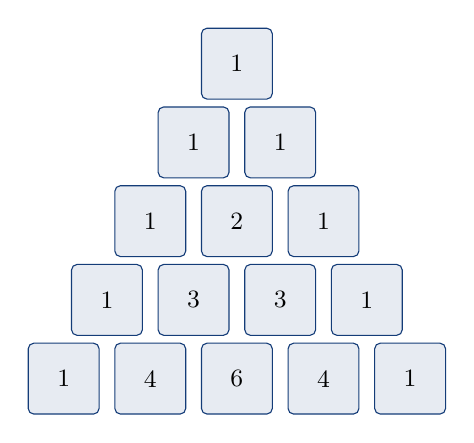
\begin{tikzpicture}[font=\small]
  \foreach \row/\vals/\y in {
    0/{1}/4.5,
    1/{1,1}/3.5,
    2/{1,2,1}/2.5,
    3/{1,3,3,1}/1.5,
    4/{1,4,6,4,1}/0.5}
  {
    \foreach [count=\col from 0] \v in \vals {
      \pgfmathsetmacro{\xpos}{(\col - \row/2) * 1.1}
      \node[draw=myblue,fill=myblue!10,minimum width=0.9cm,
            minimum height=0.9cm,rounded corners=2pt,font=\small]
        at (\xpos, \y) {\v};
    }
  }
\end{tikzpicture}
\end{center}

\begin{lstlisting}[caption={Print Pascal's Triangle --- n rows}]
public class PascalsTriangle {
    // Problem 1: Print entire Pascal's Triangle up to n rows
    public static void printTriangle(int n) {
        for (int row = 0; row < n; row++) {
            int val = 1;
            for (int col = 0; col <= row; col++) {
                System.out.print(val + " ");
                val = val * (row - col) / (col + 1);  // next element in row
            }
            System.out.println();
        }
    }

    // Problem 2: Return only the r-th row (0-indexed)
    public static int[] getRow(int r) {
        int[] row = new int[r + 1];
        row[0] = 1;
        for (int col = 1; col <= r; col++) {
            // row[col] = row[col-1] * (r - col + 1) / col
            row[col] = (int)((long) row[col - 1] * (r - col + 1) / col);
        }
        return row;
    }

    // Problem 3: Find element at row r, column c (both 0-indexed) = C(r, c)
    public static long getElement(int r, int c) {
        if (c > r - c) c = r - c;   // use symmetry: C(r,c) = C(r, r-c)
        long result = 1;
        for (int i = 0; i < c; i++) {
            result = result * (r - i) / (i + 1);
        }
        return result;
    }

    public static void main(String[] args) {
        System.out.println("Pascal's Triangle (5 rows):");
        printTriangle(5);

        System.out.print("Row 4: ");
        for (int x : getRow(4)) System.out.print(x + " ");  // 1 4 6 4 1
        System.out.println();

        System.out.println("Element at row=4, col=2: " + getElement(4, 2)); // 6
    }
}
\end{lstlisting}

\begin{dryrun}[Dry Run: getRow(4) --- row index 4 = \{1, 4, 6, 4, 1\}]
\begin{center}
\begin{tabular}{cccl}
\toprule
\textbf{col} & \textbf{row[col-1]} & \textbf{row[col] = prev $\times$ (r$-$col+1) / col} & \textbf{row}\\
\midrule
0 & ---& row[0] = 1                        & \{1,\_,\_,\_,\_\}\\
1 & 1  & $1 \times (4-1+1)/1 = 4$          & \{1,4,\_,\_,\_\}\\
2 & 4  & $4 \times (4-2+1)/2 = 6$          & \{1,4,6,\_,\_\}\\
3 & 6  & $6 \times (4-3+1)/3 = 4$          & \{1,4,6,4,\_\}\\
4 & 4  & $4 \times (4-4+1)/4 = 1$          & \{1,4,6,4,1\}\\
\bottomrule
\end{tabular}
\end{center}
\end{dryrun}

\begin{complexity}
Print $n$ rows: $O(n^2)$ time, $O(n^2)$ space\quad Get single row: $O(n)$ time, $O(n)$ space\quad Get single element: $O(c)$ time, $O(1)$ space
\end{complexity}

\section{3-Sum Problem}

\textbf{Problem:} Find all unique triplets in the array that sum to zero.

\begin{lstlisting}[caption={3-Sum --- Sort + Two Pointer, O(n$^2$)}]
import java.util.ArrayList;
import java.util.Arrays;
import java.util.List;

public class ThreeSum {
    public static List<List<Integer>> threeSum(int[] arr) {
        List<List<Integer>> result = new ArrayList<>();
        Arrays.sort(arr);   // sort first -- enables two-pointer approach
        int n = arr.length;

        for (int i = 0; i < n - 2; i++) {
            // Skip duplicate values for the fixed element
            if (i > 0 && arr[i] == arr[i - 1]) continue;

            int left  = i + 1;
            int right = n - 1;

            while (left < right) {
                int sum = arr[i] + arr[left] + arr[right];

                if (sum == 0) {
                    result.add(Arrays.asList(arr[i], arr[left], arr[right]));
                    // Skip duplicates for left and right pointers
                    while (left < right && arr[left]  == arr[left + 1])  left++;
                    while (left < right && arr[right] == arr[right - 1]) right--;
                    left++;
                    right--;
                } else if (sum < 0) {
                    left++;    // sum too small, increase left
                } else {
                    right--;   // sum too large, decrease right
                }
            }
        }
        return result;
    }

    public static void main(String[] args) {
        int[] arr = {-1, 0, 1, 2, -1, -4};
        System.out.println(threeSum(arr));
        // Output: [[-1, -1, 2], [-1, 0, 1]]
    }
}
\end{lstlisting}

\begin{dryrun}[Dry Run: arr after sort = \{$-4,-1,-1,0,1,2$\}]
\begin{center}
\begin{tabular}{ccccp{4.5cm}}
\toprule
\textbf{i} & \textbf{arr[i]} & \textbf{left} & \textbf{right} & \textbf{Action}\\
\midrule
0 & $-4$ & 1 & 5 & sum$=-3$ $\to$ left++\\
0 & $-4$ & 2 & 5 & sum$=-3$ $\to$ left++\\
0 & $-4$ & 3 & 5 & sum$=-2$ $\to$ left++\\
0 & $-4$ & 4 & 5 & sum$=-1$ $\to$ left++\\
0 & $-4$ & 5 & 5 & left$\not<$right $\to$ end\\
\midrule
1 & $-1$ & 2 & 5 & sum$=0$ \textbf{Found!} add[$-1,-1,2$]\\
1 & $-1$ & 3 & 4 & sum$=0$ \textbf{Found!} add[$-1,0,1$]\\
\midrule
2 & $-1$ & --- & --- & arr[2]==arr[1]: \textbf{skip duplicate}\\
\bottomrule
\end{tabular}
\end{center}
\textbf{Result: \{[$-1,-1,2$], [$-1,0,1$]\}}
\end{dryrun}

\begin{complexity}
Time: $O(n^2)$ --- sort $O(n\log n)$ + two-pointer for each fixed element $O(n)$\quad Space: $O(1)$ extra (excluding result)
\end{complexity}

\begin{interviewcorner}
\begin{itemize}
  \item \textbf{Brute force} is $O(n^3)$ --- three nested loops, check all triplets
  \item \textbf{HashSet} approach is also $O(n^2)$ but harder to deduplicate
  \item \textbf{Two-pointer after sort} is the standard interview solution
  \item \textbf{4-Sum:} Add one more outer loop, call 3-Sum logic inside $\to O(n^3)$
  \item Always skip duplicates after fixing each element to avoid duplicate triplets
\end{itemize}
\end{interviewcorner}

\section{Equilibrium Index}

\textbf{Problem:} Find index $i$ such that the sum of elements to its left equals the sum to its right.

\begin{lstlisting}[caption={Equilibrium Index --- Prefix Sum approach}]
public class EquilibriumIndex {
    public static int equilibrium(int[] arr) {
        int n = arr.length;

        // Total sum of array
        int totalSum = 0;
        for (int x : arr) totalSum += x;

        int leftSum = 0;
        for (int i = 0; i < n; i++) {
            // Right sum = totalSum - leftSum - arr[i]
            int rightSum = totalSum - leftSum - arr[i];

            if (leftSum == rightSum) return i;  // equilibrium found

            leftSum += arr[i];   // add current element to left sum
        }
        return -1;   // no equilibrium index
    }

    public static void main(String[] args) {
        int[] arr = {-7, 1, 5, 2, -4, 3, 0};
        System.out.println(equilibrium(arr));  // 3  (arr[3]=2; left=−1, right=−1)
    }
}
\end{lstlisting}

\begin{dryrun}[Dry Run: arr = \{$-7$, 1, 5, 2, $-4$, 3, 0\}, totalSum = 0]
\begin{center}
\begin{tabular}{ccccc}
\toprule
\textbf{i} & \textbf{arr[i]} & \textbf{leftSum} & \textbf{rightSum} & \textbf{Equal?}\\
\midrule
0 & $-7$ & 0    & $0-0-(-7)=7$   & No\\
1 & 1    & $-7$ & $0-(-7)-1=-6$  & No\\
2 & 5    & $-6$ & $0-(-6)-5=1$   & No\\
3 & 2    & $-1$ & $0-(-1)-2=-1$  & \textbf{Yes! $-1 = -1$}\\
\bottomrule
\end{tabular}
\end{center}
\textbf{Result: index 3}
\end{dryrun}

\begin{complexity}
Time: $O(n)$\quad Space: $O(1)$
\end{complexity}

%%------------------------------------------------------------
\section{Missing Elements From an Array With Duplicates}
\index{Array!missing elements with duplicates}
%%------------------------------------------------------------

\textbf{Problem (LeetCode 448 / APNA CLG 489):} Given an array \texttt{nums} of $n$ integers where values are in the range $[1, n]$ and \textit{some elements may be duplicated}, return \textbf{all integers} in $[1, n]$ that are missing from the array. The algorithm should run in $O(n)$ time and use $O(1)$ additional space.

\begin{warningbox}[Difference from ``Find the Missing Number'']
\textbf{Section 5.16} (Find the Missing Number) handled the case where the array has \textit{distinct} values and exactly \textit{one} number is missing --- solved in $O(n)$ with XOR or Gauss sum.\\[4pt]
\textbf{This problem} allows \textit{duplicates} and asks for \textit{all} missing numbers --- requires a different technique because Gauss sum and XOR no longer isolate individual missing values.
\end{warningbox}

\textbf{Approach --- Negative Marking (Index as a Hash):}

Since all values are in $[1, n]$ and indices are in $[0, n-1]$, we can use the array itself as a hash table. For each value $v$ encountered, mark \texttt{nums[v-1]} as negative (visited). Any index $i$ whose value remains positive means $i+1$ was never seen --- it is missing.

\begin{lstlisting}[caption={Missing Elements With Duplicates --- Negative Marking, O(n) time O(1) space}]
import java.util.ArrayList;
import java.util.List;

public class MissingElementsWithDuplicates {

    public static List<Integer> findMissingNumbers(int[] nums) {
        int n = nums.length;
        List<Integer> missing = new ArrayList<>();

        // --- PASS 1: Mark visited positions as negative ---
        for (int i = 0; i < n; i++) {
            // Use absolute value because the number may already have been negated
            int val = Math.abs(nums[i]);   // the value (1-indexed)
            int idx = val - 1;             // the corresponding index (0-indexed)

            if (nums[idx] > 0) {
                nums[idx] = -nums[idx];    // mark as visited (negate)
            }
            // If nums[idx] is already negative: value was already seen (duplicate)
        }

        // --- PASS 2: Collect all indices whose value is still positive ---
        for (int i = 0; i < n; i++) {
            if (nums[i] > 0) {
                missing.add(i + 1);        // index i means value (i+1) was never seen
            }
        }

        // --- Optional PASS 3: Restore original array ---
        for (int i = 0; i < n; i++) {
            nums[i] = Math.abs(nums[i]);
        }

        return missing;
    }

    public static void main(String[] args) {
        int[] arr1 = {4, 3, 2, 7, 8, 2, 3, 1};
        System.out.println(findMissingNumbers(arr1));   // [5, 6]

        int[] arr2 = {1, 1};
        System.out.println(findMissingNumbers(arr2));   // [2]

        int[] arr3 = {1, 2, 3};
        System.out.println(findMissingNumbers(arr3));   // []
    }
}
\end{lstlisting}

\begin{dryrun}[nums = \{4, 3, 2, 7, 8, 2, 3, 1\}, n = 8]
\textbf{Pass 1 --- Negative Marking:}
\begin{center}
\begin{tabular}{ccccp{4cm}}
\toprule
\textbf{i} & \textbf{nums[i]} & \textbf{val} & \textbf{idx} & \textbf{Array after marking}\\
\midrule
0 & 4  & 4 & 3 & \{4, 3, 2, \textbf{-7}, 8, 2, 3, 1\}\\
1 & 3  & 3 & 2 & \{4, 3, \textbf{-2}, -7, 8, 2, 3, 1\}\\
2 & -2 & 2 & 1 & \{4, \textbf{-3}, -2, -7, 8, 2, 3, 1\}\\
3 & -7 & 7 & 6 & \{4, -3, -2, -7, 8, 2, \textbf{-3}, 1\}\\
4 & 8  & 8 & 7 & \{4, -3, -2, -7, 8, 2, -3, \textbf{-1}\}\\
5 & 2  & 2 & 1 & already negative --- skip\\
6 & -3 & 3 & 2 & already negative --- skip\\
7 & -1 & 1 & 0 & \{\textbf{-4}, -3, -2, -7, 8, 2, -3, -1\}\\
\midrule
\multicolumn{5}{l}{Final: \{-4,-3,-2,-7,\textbf{8},\textbf{2},-3,-1\}}\\
\bottomrule
\end{tabular}
\end{center}

\vspace{4pt}
\textbf{Pass 2 --- Collect missing:}\\
Index 4 has value $+8 > 0$ $\to$ 5 is missing.\\
Index 5 has value $+2 > 0$ $\to$ 6 is missing.\\
All others are negative (their values were seen).

\textbf{Result: [5, 6]}
\end{dryrun}

\begin{center}
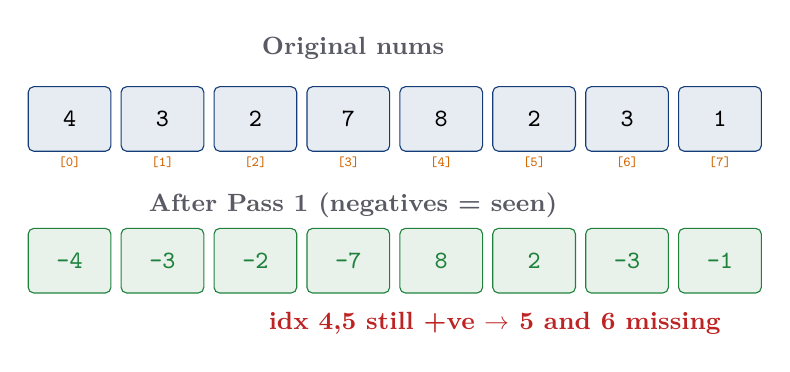
\begin{tikzpicture}[font=\small]
  % Original
  \node[text=mygray, font=\bfseries\small] at (3.6, 2.4) {Original nums};
  \foreach \v/\i in {4/0, 3/1, 2/2, 7/3, 8/4, 2/5, 3/6, 1/7}{
    \node[draw=myblue, fill=myblue!10, minimum width=1.05cm,
          minimum height=0.82cm, rounded corners=2pt, font=\ttfamily\small]
      at (\i*1.18, 1.5) {\v};
    \node[text=myorange, font=\tiny\ttfamily] at (\i*1.18, 0.95) {[\i]};
  }
  % After marking
  \node[text=mygray, font=\bfseries\small] at (3.6, 0.4) {After Pass 1 (negatives = seen)};
  \foreach \v/\i/\col in {-4/0/n,-3/1/n,-2/2/n,-7/3/n,8/4/y,2/5/y,-3/6/n,-1/7/n}{
    \ifx\col y
      \node[draw=myred, fill=myred!12, minimum width=1.05cm,
            minimum height=0.82cm, rounded corners=2pt, font=\ttfamily\small\bfseries, text=myred]
        at (\i*1.18, -0.3) {\v};
    \else
      \node[draw=mygreen, fill=mygreen!10, minimum width=1.05cm,
            minimum height=0.82cm, rounded corners=2pt, font=\ttfamily\small, text=mygreen]
        at (\i*1.18, -0.3) {\v};
    \fi
  }
  \node[text=myred, font=\small\bfseries] at (5.4+1.18*4*0, -1.1)
    {idx 4,5 still +ve $\to$ 5 and 6 missing};
\end{tikzpicture}
\end{center}

\begin{complexity}
Time: $O(n)$ --- two passes over array\quad Space: $O(1)$ extra (no auxiliary array; uses input array itself as hash)
\end{complexity}

\begin{interviewcorner}
\begin{itemize}
  \item \textbf{Why does negative marking work?} Values are in $[1,n]$ and indices in $[0,n-1]$, so value $v$ maps to index $v-1$ bijectively. Negating \texttt{nums[v-1]} encodes ``$v$ has been seen'' without losing the original magnitude
  \item \textbf{Handling duplicates:} If \texttt{nums[idx]} is already negative, the value was already marked --- we simply skip (no double-negation)
  \item \textbf{Always use \texttt{Math.abs()}} when reading during Pass 1, because earlier iterations may have already negated the value
  \item \textbf{Restore step} (Pass 3) is optional --- skip if you don't need the input array intact after the call
  \item Compared to a boolean visited array: same $O(n)$ time but $O(n)$ extra space --- negative marking achieves $O(1)$ extra space by reusing the input
\end{itemize}
\end{interviewcorner}

%%------------------------------------------------------------
\section{4-Sum Problem}

\textbf{Problem:} Find all unique quadruplets in the array that sum to a given target.

\textbf{Approach:} Fix two elements with nested loops, then apply the Two-Pointer technique on the remaining sorted subarray --- same idea as 3-Sum with one more outer loop.

\begin{lstlisting}[caption={4-Sum --- Fix Two + Two Pointer, O(n$^3$)}]
import java.util.ArrayList;
import java.util.Arrays;
import java.util.List;

public class FourSum {
    public static List<List<Integer>> fourSum(int[] arr, int target) {
        List<List<Integer>> result = new ArrayList<>();
        Arrays.sort(arr);           // sort first
        int n = arr.length;

        for (int i = 0; i < n - 3; i++) {
            if (i > 0 && arr[i] == arr[i - 1]) continue; // skip i duplicates

            for (int j = i + 1; j < n - 2; j++) {
                if (j > i + 1 && arr[j] == arr[j - 1]) continue; // skip j duplicates

                int left  = j + 1;
                int right = n - 1;

                while (left < right) {
                    long sum = (long) arr[i] + arr[j] + arr[left] + arr[right];

                    if (sum == target) {
                        result.add(Arrays.asList(arr[i], arr[j], arr[left], arr[right]));
                        while (left < right && arr[left]  == arr[left + 1])  left++;
                        while (left < right && arr[right] == arr[right - 1]) right--;
                        left++;
                        right--;
                    } else if (sum < target) {
                        left++;
                    } else {
                        right--;
                    }
                }
            }
        }
        return result;
    }

    public static void main(String[] args) {
        int[] arr = {1, 0, -1, 0, -2, 2};
        System.out.println(fourSum(arr, 0));
        // Output: [[-2,-1,1,2], [-2,0,0,2], [-1,0,0,1]]
    }
}
\end{lstlisting}

\begin{complexity}
Time: $O(n^3)$ --- two fixed pointers + two-pointer pass\quad Space: $O(1)$ extra (excluding output)
\end{complexity}

\begin{interviewcorner}
\begin{itemize}
  \item Use \texttt{long} for the sum to avoid integer overflow (4 ints can exceed \texttt{int} range)
  \item The deduplication logic (skip same values for i, j, left, right) is the tricky part
  \item Pattern generalises: $k$-Sum --- fix $k-2$ elements, do Two-Pointer on the rest: $O(n^{k-1})$
\end{itemize}
\end{interviewcorner}

%%------------------------------------------------------------
\section{Next Permutation}

\textbf{Problem:} Find the next lexicographically greater permutation of an array. If already the largest (fully descending), return the smallest (fully ascending).

\textbf{Example:} \texttt{[1,2,3]} $\to$ \texttt{[1,3,2]}\quad \texttt{[3,2,1]} $\to$ \texttt{[1,2,3]}\quad \texttt{[1,1,5]} $\to$ \texttt{[1,5,1]}

\textbf{Algorithm (3 steps, all $O(n)$):}
\begin{enumerate}
  \item Find the \textbf{pivot}: scan right to left, find first index $i$ where \texttt{arr[i] < arr[i+1]}
  \item Find the \textbf{successor}: scan right to left, find first element $>$ \texttt{arr[i]}; swap with \texttt{arr[i]}
  \item \textbf{Reverse} the suffix starting at $i+1$ (was descending; reversing gives ascending = smallest)
\end{enumerate}

\begin{lstlisting}[caption={Next Permutation --- O(n) time O(1) space}]
public class NextPermutation {
    public static void nextPermutation(int[] arr) {
        int n = arr.length;

        // Step 1: Find pivot (first from right where arr[i] < arr[i+1])
        int pivot = -1;
        for (int i = n - 2; i >= 0; i--) {
            if (arr[i] < arr[i + 1]) {
                pivot = i;
                break;
            }
        }

        // No pivot means fully descending: reverse whole array
        if (pivot == -1) {
            reverse(arr, 0, n - 1);
            return;
        }

        // Step 2: Find rightmost element > arr[pivot] and swap
        for (int i = n - 1; i > pivot; i--) {
            if (arr[i] > arr[pivot]) {
                int temp   = arr[pivot];
                arr[pivot] = arr[i];
                arr[i]     = temp;
                break;
            }
        }

        // Step 3: Reverse suffix after pivot
        reverse(arr, pivot + 1, n - 1);
    }

    private static void reverse(int[] arr, int start, int end) {
        while (start < end) {
            int temp   = arr[start];
            arr[start] = arr[end];
            arr[end]   = temp;
            start++; end--;
        }
    }

    public static void main(String[] args) {
        int[] arr1 = {1, 2, 3};  nextPermutation(arr1);
        for (int x : arr1) System.out.print(x + " "); // 1 3 2
        System.out.println();

        int[] arr2 = {3, 2, 1};  nextPermutation(arr2);
        for (int x : arr2) System.out.print(x + " "); // 1 2 3
        System.out.println();
    }
}
\end{lstlisting}

\begin{dryrun}[Next Permutation of \{2, 1, 5, 4, 3\}]
\begin{center}
\begin{tabular}{lp{5cm}l}
\toprule
\textbf{Step} & \textbf{Action} & \textbf{Array}\\
\midrule
Initial       & ---                                          & \{2,1,5,4,3\}\\
Step 1        & arr[1]=1 $<$ arr[2]=5 $\to$ pivot=1        & pivot at index 1\\
Step 2        & rightmost $>$1: arr[4]=3; swap[1]\&[4]      & \{2,3,5,4,1\}\\
Step 3        & reverse suffix [2..4]: \{5,4,1\}$\to$\{1,4,5\} & \{2,3,1,4,5\}\\
\bottomrule
\end{tabular}
\end{center}
\textbf{Result: \{2, 3, 1, 4, 5\}}
\end{dryrun}

\begin{complexity}
Time: $O(n)$ --- three linear passes\quad Space: $O(1)$ --- in-place
\end{complexity}

\begin{interviewcorner}
\begin{itemize}
  \item This is exactly \texttt{std::next\_permutation} from C++ STL
  \item \textbf{Why reverse the suffix?} After step 2, suffix is still descending. Reversing gives the smallest (ascending) arrangement
  \item Asked at Google, Facebook, Amazon, Microsoft
  \item Follow-up: \textit{Previous permutation} --- mirror logic: find first \texttt{arr[i] > arr[i+1]}, swap with rightmost smaller, reverse suffix
\end{itemize}
\end{interviewcorner}

%%############################################################
%%############################################################
\chapter{2-D Arrays (Matrices)}
\index{2-D Arrays}\index{Matrix}
%%############################################################

A \textbf{2-D array} (matrix) is an array of arrays --- a table of rows and columns. It is the gateway to grid problems, image processing, graph adjacency matrices, and dynamic programming tables.

\begin{definitionbox}{2-D Array}
A 2-D array \texttt{int[][] mat} of size $m \times n$ has $m$ rows and $n$ columns. Element at row $i$, column $j$ is accessed as \texttt{mat[i][j]} in $O(1)$.
\end{definitionbox}

\section{Memory Representation}
\index{Matrix!memory}

\begin{center}
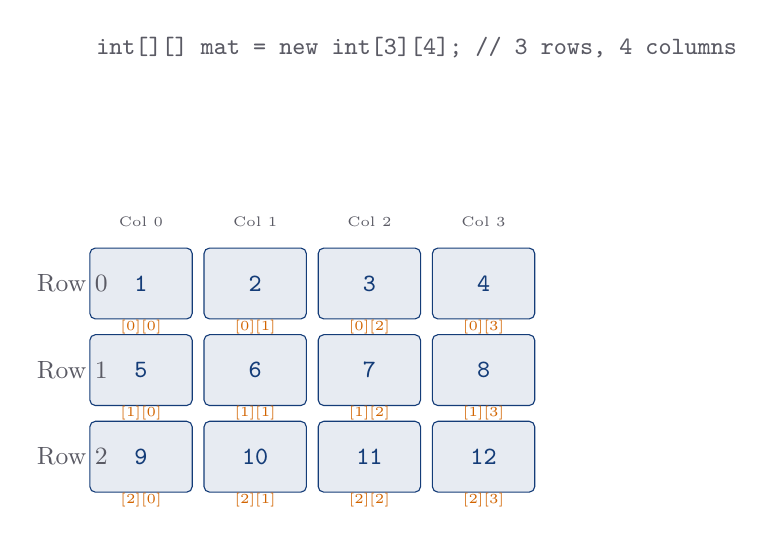
\begin{tikzpicture}[font=\small]
  % Grid label
  \node[text=mygray, font=\ttfamily\small] at (3.5, 3.0)
    {int[][] mat = new int[3][4];  // 3 rows, 4 columns};

  % Draw cells
  \foreach \r in {0,1,2}{
    \foreach \c in {0,1,2,3}{
      \pgfmathtruncatemacro{\val}{(\r*4+\c+1)}
      \node[draw=myblue, fill=myblue!10, minimum width=1.3cm, minimum height=0.9cm,
            rounded corners=2pt, font=\ttfamily\small, text=myblue]
        at (\c*1.45, -\r*1.1) {\val};
      \node[font=\tiny, text=myorange] at (\c*1.45, -\r*1.1-0.55)
        {[\r][\c]};
    }
  }
  % Row labels
  \foreach \r/\rn in {0/Row 0, 1/Row 1, 2/Row 2}{
    \node[left=0.2cm, text=mygray, font=\small] at (-0.1, -\r*1.1) {\rn};
  }
  % Column labels
  \foreach \c/\cn in {0/Col 0, 1/Col 1, 2/Col 2, 3/Col 3}{
    \node[above=0.1cm, text=mygray, font=\tiny] at (\c*1.45, 0.5) {\cn};
  }
\end{tikzpicture}
\end{center}

\textbf{Key Facts:}
\begin{itemize}
  \item \texttt{mat.length} $\to$ number of rows
  \item \texttt{mat[0].length} $\to$ number of columns
  \item Total elements: rows $\times$ columns
  \item Stored in \textbf{row-major order} in Java (each row is a separate 1-D array)
  \item Access \texttt{mat[i][j]}: $O(1)$ --- direct index calculation
\end{itemize}

\section{Declaring and Initialising a 2-D Array}
\index{Matrix!declaration}

\begin{lstlisting}[caption={Declaring, initialising, and traversing a 2-D array}]
public class MatrixBasics {
    public static void main(String[] args) {

        // Way 1: Declare size only (filled with 0s)
        int[][] mat1 = new int[3][4];   // 3 rows, 4 columns

        // Way 2: Declare with values (jagged is also allowed in Java)
        int[][] mat2 = {
            {1, 2, 3},
            {4, 5, 6},
            {7, 8, 9}
        };

        // Accessing a single element
        System.out.println(mat2[1][2]);   // 6  (row 1, col 2)

        // Length
        System.out.println("Rows : " + mat2.length);       // 3
        System.out.println("Cols : " + mat2[0].length);    // 3

        // Traversal: nested for loop
        System.out.println("Full matrix:");
        for (int i = 0; i < mat2.length; i++) {
            for (int j = 0; j < mat2[i].length; j++) {
                System.out.print(mat2[i][j] + " ");
            }
            System.out.println();   // new row = new line
        }
    }
}
\end{lstlisting}

\begin{dryrun}[Traversal of 3$\times$3 matrix \{\{1,2,3\},\{4,5,6\},\{7,8,9\}\}]
\begin{center}
\begin{tabular}{cccl}
\toprule
\textbf{i (row)} & \textbf{j (col)} & \textbf{mat[i][j]} & \textbf{Output}\\
\midrule
0 & 0,1,2 & 1, 2, 3 & \texttt{1 2 3}\\
1 & 0,1,2 & 4, 5, 6 & \texttt{4 5 6}\\
2 & 0,1,2 & 7, 8, 9 & \texttt{7 8 9}\\
\bottomrule
\end{tabular}
\end{center}
\end{dryrun}

\begin{complexity}
Traversal: Time $O(m \times n)$ \quad Space $O(1)$
\end{complexity}

\section{Print Diagonal Elements}
\index{Matrix!diagonal}

\textbf{Problem:} Print all elements on the main diagonal of a square matrix. The main diagonal consists of elements where row index $=$ column index: \texttt{mat[i][i]}.

\begin{center}
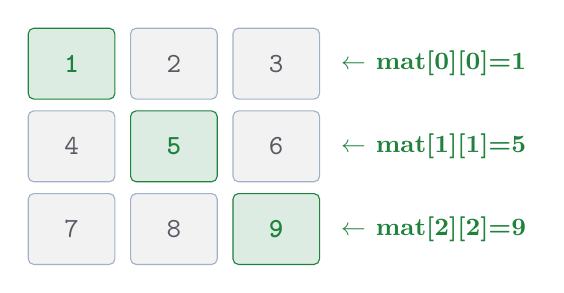
\begin{tikzpicture}[font=\small]
  \foreach \r in {0,1,2}{
    \foreach \c in {0,1,2}{
      \pgfmathtruncatemacro{\val}{(\r*3+\c+1)}
      \ifnum\r=\c
        \node[draw=mygreen, fill=mygreen!15, minimum width=1.1cm,
              minimum height=0.9cm, rounded corners=2pt,
              font=\ttfamily\bfseries, text=mygreen]
          at (\c*1.3, -\r*1.05) {\val};
      \else
        \node[draw=myblue!40, fill=gray!10, minimum width=1.1cm,
              minimum height=0.9cm, rounded corners=2pt, font=\ttfamily, text=mygray]
          at (\c*1.3, -\r*1.05) {\val};
      \fi
    }
  }
  \node[right=0.4cm, text=mygreen, font=\small\bfseries] at (2.9, 0)
    {$\leftarrow$ mat[0][0]=1};
  \node[right=0.4cm, text=mygreen, font=\small\bfseries] at (2.9, -1.05)
    {$\leftarrow$ mat[1][1]=5};
  \node[right=0.4cm, text=mygreen, font=\small\bfseries] at (2.9, -2.10)
    {$\leftarrow$ mat[2][2]=9};
\end{tikzpicture}
\end{center}

\begin{lstlisting}[caption={Print Diagonal Elements}]
public class PrintDiagonal {
    public static void printDiagonal(int[][] mat) {
        // Only valid for square matrix (rows == cols)
        for (int i = 0; i < mat.length; i++) {
            System.out.print(mat[i][i] + " ");   // row index == col index
        }
        System.out.println();
    }

    public static void main(String[] args) {
        int[][] mat = {
            {1, 2, 3},
            {4, 5, 6},
            {7, 8, 9}
        };
        printDiagonal(mat);   // Output: 1 5 9
    }
}
\end{lstlisting}

\begin{complexity}
Time: $O(n)$ for an $n \times n$ matrix \quad Space: $O(1)$
\end{complexity}

\section{Sum of Diagonal Elements}
\index{Matrix!diagonal sum}

\begin{lstlisting}[caption={Diagonal Sum --- main diagonal only}]
public class DiagonalSum {
    public static int diagonalSum(int[][] mat) {
        int sum = 0;
        for (int i = 0; i < mat.length; i++) {
            sum += mat[i][i];   // accumulate diagonal elements
        }
        return sum;
    }

    public static void main(String[] args) {
        int[][] mat = {
            {1, 2, 3},
            {4, 5, 6},
            {7, 8, 9}
        };
        System.out.println("Diagonal sum = " + diagonalSum(mat));  // 15
    }
}
\end{lstlisting}

\begin{dryrun}[arr = \{\{1,2,3\},\{4,5,6\},\{7,8,9\}\}]
\begin{center}
\begin{tabular}{cccc}
\toprule
\textbf{i} & \textbf{mat[i][i]} & \textbf{sum before} & \textbf{sum after}\\
\midrule
0 & 1 & 0  & 1\\
1 & 5 & 1  & 6\\
2 & 9 & 6  & 15\\
\bottomrule
\end{tabular}
\end{center}
\textbf{Result: 15}
\end{dryrun}

\begin{tipbox}[Both Diagonals Sum]
For the \textbf{anti-diagonal} (top-right to bottom-left), the index is \texttt{mat[i][n-1-i]}. To sum both diagonals, add both --- but if $n$ is odd, subtract \texttt{mat[n/2][n/2]} once (counted twice in the middle).
\end{tipbox}

\begin{complexity}
Time: $O(n)$ \quad Space: $O(1)$
\end{complexity}

\section{Search Element in a Matrix}
\index{Matrix!search}

\textbf{Problem:} Given an $m \times n$ matrix, return \texttt{true} if target exists, else \texttt{false}.

\subsection{Brute Force --- Check All Elements}

\begin{lstlisting}[caption={Search in Matrix --- Brute Force O(m*n)}]
public class SearchMatrix {
    public static boolean search(int[][] mat, int target) {
        for (int i = 0; i < mat.length; i++) {
            for (int j = 0; j < mat[0].length; j++) {
                if (mat[i][j] == target) {
                    return true;    // found
                }
            }
        }
        return false;               // not found
    }

    public static void main(String[] args) {
        int[][] mat = {
            {1,  4,  7,  11},
            {2,  5,  8,  12},
            {3,  6,  9,  16},
            {10, 13, 14, 17}
        };
        System.out.println(search(mat, 5));   // true
        System.out.println(search(mat, 20));  // false
    }
}
\end{lstlisting}

\begin{complexity}
Time: $O(m \times n)$ \quad Space: $O(1)$
\end{complexity}

\subsection{Optimised --- Staircase Search (Sorted Matrix)}

If each row is sorted left-to-right and each column is sorted top-to-bottom, we can search in $O(m + n)$ by starting from the \textbf{top-right corner}.

\begin{lstlisting}[caption={Search in Row-Column Sorted Matrix --- O(m+n)}]
public class SearchSortedMatrix {
    public static boolean searchSorted(int[][] mat, int target) {
        int row = 0;
        int col = mat[0].length - 1;   // start at top-right corner

        while (row < mat.length && col >= 0) {
            if (mat[row][col] == target) {
                return true;
            } else if (mat[row][col] > target) {
                col--;    // current value too large: move left
            } else {
                row++;    // current value too small: move down
            }
        }
        return false;
    }

    public static void main(String[] args) {
        int[][] mat = {
            {1,  4,  7,  11},
            {2,  5,  8,  12},
            {3,  6,  9,  16},
            {10, 13, 14, 17}
        };
        System.out.println(searchSorted(mat, 5));   // true
        System.out.println(searchSorted(mat, 20));  // false
    }
}
\end{lstlisting}

\begin{dryrun}[Searching for 5 in the matrix above (start top-right = mat[0][3] = 11)]
\begin{center}
\begin{tabular}{cccl}
\toprule
\textbf{row} & \textbf{col} & \textbf{mat[row][col]} & \textbf{Action}\\
\midrule
0 & 3 & 11 & $11 > 5$: col-- \\
0 & 2 & 7  & $7 > 5$: col--  \\
0 & 1 & 4  & $4 < 5$: row++  \\
1 & 1 & 5  & $5 = 5$: \textbf{Found!} return true\\
\bottomrule
\end{tabular}
\end{center}
\end{dryrun}

\begin{interviewcorner}
\textbf{Why top-right corner?} From top-right, moving left decreases value, moving down increases value --- gives us a clear binary decision at every step. Starting from top-left or bottom-right would not give this property.
\end{interviewcorner}

\begin{complexity}
Brute Force: $O(m \times n)$\quad Staircase (sorted matrix): $O(m + n)$\quad Space: $O(1)$ both
\end{complexity}

\section{Check if Matrix is Symmetric}
\index{Matrix!symmetric}

A matrix is \textbf{symmetric} if \texttt{mat[i][j] == mat[j][i]} for all $i, j$. Only applicable to square matrices.

\begin{lstlisting}[caption={Check Symmetric --- only compare upper triangle, O(n$^2$/2)}]
public class SymmetricMatrix {
    public static boolean isSymmetric(int[][] mat) {
        int n = mat.length;
        // Only check upper triangle (above diagonal)
        for (int i = 0; i < n; i++) {
            for (int j = i + 1; j < n; j++) {   // j starts from i+1
                if (mat[i][j] != mat[j][i]) {
                    return false;   // violation found
                }
            }
        }
        return true;
    }

    public static void main(String[] args) {
        int[][] sym = {
            {1, 2, 3},
            {2, 5, 6},
            {3, 6, 9}
        };
        int[][] notSym = {
            {1, 2, 3},
            {4, 5, 6},
            {7, 8, 9}
        };
        System.out.println(isSymmetric(sym));     // true
        System.out.println(isSymmetric(notSym));  // false
    }
}
\end{lstlisting}

\begin{dryrun}[Check sym matrix: only upper triangle pairs]
\begin{center}
\begin{tabular}{ccccl}
\toprule
\textbf{i} & \textbf{j} & \textbf{mat[i][j]} & \textbf{mat[j][i]} & \textbf{Equal?}\\
\midrule
0 & 1 & 2 & 2 & Yes\\
0 & 2 & 3 & 3 & Yes\\
1 & 2 & 6 & 6 & Yes\\
\multicolumn{5}{l}{No violation found $\to$ \textbf{Symmetric}}\\
\bottomrule
\end{tabular}
\end{center}
\end{dryrun}

\begin{tipbox}[Why start j from i+1?]
The diagonal (\texttt{mat[i][i]}) is always equal to itself. Below-diagonal pairs are mirror images of above-diagonal --- checking both would be redundant. Starting $j$ from $i+1$ checks each pair exactly once: $O(n^2/2) \approx O(n^2)$.
\end{tipbox}

\begin{complexity}
Time: $O(n^2)$ (half the pairs) \quad Space: $O(1)$
\end{complexity}

\section{Matrix Transpose}
\index{Matrix!transpose}

The \textbf{transpose} of a matrix flips it over its diagonal: row $i$ becomes column $i$. \texttt{mat[i][j]} and \texttt{mat[j][i]} are swapped.

\begin{center}
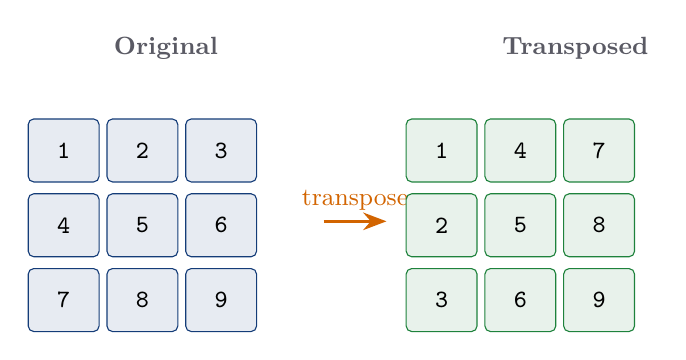
\begin{tikzpicture}[font=\small]
  % Original
  \node[text=mygray, font=\bfseries\small] at (1.3, 1.3) {Original};
  \foreach \r/\vals in {0/{1,2,3}, 1/{4,5,6}, 2/{7,8,9}}{
    \foreach [count=\c from 0] \v in \vals{
      \node[draw=myblue, fill=myblue!10, minimum width=0.9cm,
            minimum height=0.8cm, rounded corners=2pt, font=\ttfamily\small]
        at (\c*1.0, -\r*0.95) {\v};
    }
  }
  % Arrow
  \draw[myorange, -{Stealth}, very thick] (3.3, -0.9) -- (4.1, -0.9)
    node[above, midway, font=\small, text=myorange]{transpose};
  % Transposed
  \node[text=mygray, font=\bfseries\small] at (6.5, 1.3) {Transposed};
  \foreach \r/\vals in {0/{1,4,7}, 1/{2,5,8}, 2/{3,6,9}}{
    \foreach [count=\c from 0] \v in \vals{
      \node[draw=mygreen, fill=mygreen!10, minimum width=0.9cm,
            minimum height=0.8cm, rounded corners=2pt, font=\ttfamily\small]
        at (4.8+\c*1.0, -\r*0.95) {\v};
    }
  }
\end{tikzpicture}
\end{center}

\begin{lstlisting}[caption={Matrix Transpose --- in-place, swap upper triangle only}]
public class Transpose {
    public static void transpose(int[][] mat) {
        int n = mat.length;
        // Only swap above-diagonal elements (j > i)
        // If we swapped all, we'd undo every swap!
        for (int i = 0; i < n; i++) {
            for (int j = i + 1; j < n; j++) {
                int temp    = mat[i][j];
                mat[i][j]   = mat[j][i];
                mat[j][i]   = temp;
            }
        }
    }

    public static void main(String[] args) {
        int[][] mat = {
            {1, 2, 3},
            {4, 5, 6},
            {7, 8, 9}
        };
        transpose(mat);
        // mat is now:
        // 1 4 7
        // 2 5 8
        // 3 6 9
        for (int[] row : mat) {
            for (int v : row) System.out.print(v + " ");
            System.out.println();
        }
    }
}
\end{lstlisting}

\begin{dryrun}[Transpose of \{\{1,2,3\},\{4,5,6\},\{7,8,9\}\}]
\begin{center}
\begin{tabular}{cccl}
\toprule
\textbf{i} & \textbf{j} & \textbf{Swap} & \textbf{Effect}\\
\midrule
0 & 1 & mat[0][1] $\leftrightarrow$ mat[1][0] & 2 $\leftrightarrow$ 4\\
0 & 2 & mat[0][2] $\leftrightarrow$ mat[2][0] & 3 $\leftrightarrow$ 7\\
1 & 2 & mat[1][2] $\leftrightarrow$ mat[2][1] & 6 $\leftrightarrow$ 8\\
\bottomrule
\end{tabular}
\end{center}
\textbf{Result:} \{\{1,4,7\}, \{2,5,8\}, \{3,6,9\}\}
\end{dryrun}

\begin{complexity}
Time: $O(n^2)$ \quad Space: $O(1)$ --- in-place, only one \texttt{temp} variable
\end{complexity}

\section{Rotate Matrix 90\textdegree{} Clockwise}
\index{Matrix!rotate 90 clockwise}

\textbf{Key insight:} Rotate $90°$ clockwise = \textbf{Transpose} + \textbf{Reverse each row}.

\begin{center}
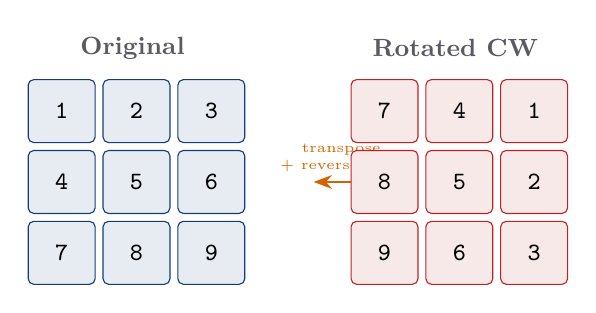
\begin{tikzpicture}[font=\small, node distance=0.4cm]
  \foreach \r/\vals in {0/{1,2,3}, 1/{4,5,6}, 2/{7,8,9}}{
    \foreach [count=\c from 0] \v in \vals{
      \node[draw=myblue, fill=myblue!10, minimum width=0.85cm,
            minimum height=0.8cm, rounded corners=2pt, font=\ttfamily\small]
        at (\c*0.95, -\r*0.90) {\v};
    }
  }
  \node[text=mygray, font=\bfseries\small] at (0.9, 0.8) {Original};

  \draw[myorange,{Stealth}-{Stealth}, thick] (3.2,-0.9) -- (3.9,-0.9)
    node[above, midway, font=\tiny, text=myorange, align=center]{transpose\\+ reverse rows};

  \foreach \r/\vals in {0/{7,4,1}, 1/{8,5,2}, 2/{9,6,3}}{
    \foreach [count=\c from 0] \v in \vals{
      \node[draw=myred, fill=myred!10, minimum width=0.85cm,
            minimum height=0.8cm, rounded corners=2pt, font=\ttfamily\small]
        at (4.1+\c*0.95, -\r*0.90) {\v};
    }
  }
  \node[text=mygray, font=\bfseries\small] at (5.0, 0.8) {Rotated CW};
\end{tikzpicture}
\end{center}

\begin{lstlisting}[caption={Rotate Matrix 90° Clockwise --- Transpose + Reverse Rows}]
public class RotateCW {
    public static void rotate(int[][] mat) {
        int n = mat.length;

        // Step 1: Transpose the matrix
        for (int i = 0; i < n; i++) {
            for (int j = i + 1; j < n; j++) {
                int temp  = mat[i][j];
                mat[i][j] = mat[j][i];
                mat[j][i] = temp;
            }
        }

        // Step 2: Reverse each row
        for (int i = 0; i < n; i++) {
            int left = 0, right = n - 1;
            while (left < right) {
                int temp       = mat[i][left];
                mat[i][left]   = mat[i][right];
                mat[i][right]  = temp;
                left++;
                right--;
            }
        }
    }

    public static void main(String[] args) {
        int[][] mat = {
            {1, 2, 3},
            {4, 5, 6},
            {7, 8, 9}
        };
        rotate(mat);
        for (int[] row : mat) {
            for (int v : row) System.out.print(v + " ");
            System.out.println();
        }
        // Output:
        // 7 4 1
        // 8 5 2
        // 9 6 3
    }
}
\end{lstlisting}

\begin{dryrun}[Rotate \{\{1,2,3\},\{4,5,6\},\{7,8,9\}\} clockwise]
\begin{center}
\begin{tabular}{lll}
\toprule
\textbf{Step} & \textbf{Operation} & \textbf{Matrix State}\\
\midrule
Initial        & ---                 & \{\{1,2,3\},\{4,5,6\},\{7,8,9\}\}\\
After Transpose& swap upper triangle & \{\{1,4,7\},\{2,5,8\},\{3,6,9\}\}\\
After Rev Row 0& reverse \{1,4,7\}   & \{\{7,4,1\},\{2,5,8\},\{3,6,9\}\}\\
After Rev Row 1& reverse \{2,5,8\}   & \{\{7,4,1\},\{8,5,2\},\{3,6,9\}\}\\
After Rev Row 2& reverse \{3,6,9\}   & \{\{7,4,1\},\{8,5,2\},\{9,6,3\}\}\\
\bottomrule
\end{tabular}
\end{center}
\end{dryrun}

\begin{complexity}
Time: $O(n^2)$ \quad Space: $O(1)$ --- fully in-place
\end{complexity}

\section{Rotate Matrix 90\textdegree{} Anticlockwise}
\index{Matrix!rotate 90 anticlockwise}

\textbf{Key insight:} Rotate $90°$ anticlockwise = \textbf{Transpose} + \textbf{Reverse each column}.

\begin{lstlisting}[caption={Rotate Matrix 90° Anticlockwise --- Transpose + Reverse Columns}]
public class RotateCCW {
    public static void rotateAnti(int[][] mat) {
        int n = mat.length;

        // Step 1: Transpose
        for (int i = 0; i < n; i++) {
            for (int j = i + 1; j < n; j++) {
                int temp  = mat[i][j];
                mat[i][j] = mat[j][i];
                mat[j][i] = temp;
            }
        }

        // Step 2: Reverse each COLUMN (not row!)
        for (int j = 0; j < n; j++) {
            int top = 0, bottom = n - 1;
            while (top < bottom) {
                int temp        = mat[top][j];
                mat[top][j]     = mat[bottom][j];
                mat[bottom][j]  = temp;
                top++;
                bottom--;
            }
        }
    }

    public static void main(String[] args) {
        int[][] mat = {
            {1, 2, 3},
            {4, 5, 6},
            {7, 8, 9}
        };
        rotateAnti(mat);
        for (int[] row : mat) {
            for (int v : row) System.out.print(v + " ");
            System.out.println();
        }
        // Output:
        // 3 6 9
        // 2 5 8
        // 1 4 7
    }
}
\end{lstlisting}

\begin{dryrun}[Rotate \{\{1,2,3\},\{4,5,6\},\{7,8,9\}\} anticlockwise]
\begin{center}
\begin{tabular}{lll}
\toprule
\textbf{Step} & \textbf{Operation} & \textbf{Matrix State}\\
\midrule
Initial           & ---                    & \{\{1,2,3\},\{4,5,6\},\{7,8,9\}\}\\
After Transpose   & swap upper triangle    & \{\{1,4,7\},\{2,5,8\},\{3,6,9\}\}\\
After Rev Col 0   & reverse col \{1,2,3\}  & \{\{3,4,7\},\{2,5,8\},\{1,6,9\}\}\\
After Rev Col 1   & reverse col \{4,5,6\}  & \{\{3,6,7\},\{2,5,8\},\{1,4,9\}\}\\
After Rev Col 2   & reverse col \{7,8,9\}  & \{\{3,6,9\},\{2,5,8\},\{1,4,7\}\}\\
\bottomrule
\end{tabular}
\end{center}
\end{dryrun}

\begin{tipbox}[CW vs CCW Memory Trick]
\textbf{Clockwise:} Transpose $\to$ Reverse \textbf{rows}\\
\textbf{Anticlockwise:} Transpose $\to$ Reverse \textbf{columns}
\end{tipbox}

\begin{complexity}
Time: $O(n^2)$ \quad Space: $O(1)$
\end{complexity}

\section{Spiral Matrix --- Print in Spiral Order}
\index{Matrix!spiral order}

\textbf{Problem:} Print all elements of an $m \times n$ matrix in \textbf{clockwise spiral order}, starting from the top-left corner.

\begin{center}
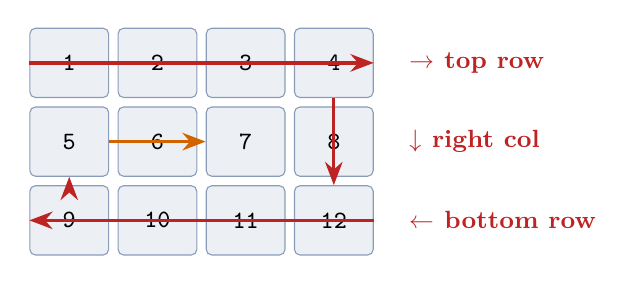
\begin{tikzpicture}[font=\small]
  % Draw the 3x4 matrix
  \foreach \r/\vals in {0/{1,2,3,4}, 1/{5,6,7,8}, 2/{9,10,11,12}}{
    \foreach [count=\c from 0] \v in \vals{
      \node[draw=myblue!50, fill=myblue!8, minimum width=1.0cm,
            minimum height=0.88cm, rounded corners=2pt, font=\ttfamily\small]
        (m\r\c) at (\c*1.12, -\r*1.0) {\v};
    }
  }
  % Spiral arrows
  \draw[myred, very thick, -{Stealth}]
    (m00.west) -- (m03.east);
  \draw[myred, very thick, -{Stealth}]
    (m03.south) -- (m23.north);
  \draw[myred, very thick, -{Stealth}]
    (m23.east) -- (m20.west);
  \draw[myred, very thick, -{Stealth}]
    (m20.north) -- (m10.south);
  \draw[myorange, very thick, -{Stealth}]
    (m10.east) -- (m12.west);
  % Labels
  \node[right=0.3cm, text=myred, font=\small\bfseries] at (3.9, 0)
    {$\to$ top row};
  \node[right=0.3cm, text=myred, font=\small\bfseries] at (3.9, -1.0)
    {$\downarrow$ right col};
  \node[right=0.3cm, text=myred, font=\small\bfseries] at (3.9, -2.0)
    {$\leftarrow$ bottom row};
\end{tikzpicture}
\end{center}

\textbf{Approach:} Maintain four boundaries: \texttt{top}, \texttt{bottom}, \texttt{left}, \texttt{right}. Traverse all four sides, then shrink boundaries inward. Repeat until boundaries cross.

\begin{lstlisting}[caption={Spiral Matrix --- boundary shrinking approach}]
import java.util.ArrayList;
import java.util.List;

public class SpiralMatrix {
    public static List<Integer> spiralOrder(int[][] mat) {
        List<Integer> result = new ArrayList<>();
        if (mat == null || mat.length == 0) return result;

        int top    = 0;
        int bottom = mat.length - 1;
        int left   = 0;
        int right  = mat[0].length - 1;

        while (top <= bottom && left <= right) {

            // 1. Traverse top row (left to right)
            for (int j = left; j <= right; j++)
                result.add(mat[top][j]);
            top++;

            // 2. Traverse right column (top to bottom)
            for (int i = top; i <= bottom; i++)
                result.add(mat[i][right]);
            right--;

            // 3. Traverse bottom row (right to left) -- if still valid
            if (top <= bottom) {
                for (int j = right; j >= left; j--)
                    result.add(mat[bottom][j]);
                bottom--;
            }

            // 4. Traverse left column (bottom to top) -- if still valid
            if (left <= right) {
                for (int i = bottom; i >= top; i--)
                    result.add(mat[i][left]);
                left++;
            }
        }
        return result;
    }

    public static void main(String[] args) {
        int[][] mat = {
            {1,  2,  3,  4},
            {5,  6,  7,  8},
            {9, 10, 11, 12}
        };
        System.out.println(spiralOrder(mat));
        // Output: [1, 2, 3, 4, 8, 12, 11, 10, 9, 5, 6, 7]
    }
}
\end{lstlisting}

\begin{dryrun}[Spiral order of 3$\times$4 matrix]
\begin{center}
\begin{tabular}{llll}
\toprule
\textbf{Pass} & \textbf{Direction} & \textbf{Elements} & \textbf{Boundary after}\\
\midrule
1 & Top row $\to$    & 1, 2, 3, 4    & top=1\\
2 & Right col $\downarrow$ & 8, 12    & right=2\\
3 & Bottom row $\leftarrow$ & 11, 10, 9 & bottom=1\\
4 & Left col $\uparrow$    & 5          & left=1\\
5 & Top row $\to$    & 6, 7          & top=2 (done)\\
\bottomrule
\end{tabular}
\end{center}
\textbf{Output: [1, 2, 3, 4, 8, 12, 11, 10, 9, 5, 6, 7]}
\end{dryrun}

\begin{complexity}
Time: $O(m \times n)$ --- every element visited exactly once\quad Space: $O(1)$ extra (output list not counted)
\end{complexity}

\begin{interviewcorner}
\begin{itemize}
  \item The guard conditions \texttt{if (top <= bottom)} and \texttt{if (left <= right)} before steps 3 and 4 prevent double-counting rows/columns in non-square matrices
  \item Common follow-up: generate an $n \times n$ spiral matrix (fill values in spiral order)
  \item Appears in: Amazon, Google, Microsoft interviews
\end{itemize}
\end{interviewcorner}

\section{2-D Arrays --- Quick Revision}
\index{Matrix!revision}
%%------------------------------------------------------------

\begin{center}
\renewcommand{\arraystretch}{1.55}
\setlength{\tabcolsep}{9pt}
\begin{tabular}{
  !{\color{myblue}\vrule width 1.2pt}
  >{\bfseries}p{4.8cm}
  !{\color{myblue!40}\vrule}
  p{2.6cm}
  !{\color{myblue!40}\vrule}
  p{5.8cm}
  !{\color{myblue}\vrule width 1.2pt}
}
\arrayrulecolor{myblue}\hline
\rowcolor{myblue}
\color{white}\textbf{Problem} &
\color{white}\textbf{Time} &
\color{white}\textbf{Key Idea}\\
\arrayrulecolor{myblue}\hline
\rowcolor{myblue!8}
Print Diagonal        & $O(n)$       & \texttt{mat[i][i]}\\
\rowcolor{white}
Diagonal Sum          & $O(n)$       & Accumulate \texttt{mat[i][i]}\\
\rowcolor{myblue!8}
Search (brute)        & $O(mn)$      & Nested loop check all\\
\rowcolor{white}
Search (sorted)       & $O(m+n)$     & Top-right: left or down\\
\rowcolor{myblue!8}
Symmetric Check       & $O(n^2)$     & \texttt{mat[i][j] == mat[j][i]}\\
\rowcolor{white}
Transpose             & $O(n^2)$     & Swap \texttt{mat[i][j]} and \texttt{mat[j][i]}\\
\rowcolor{myblue!8}
Rotate CW 90°         & $O(n^2)$     & Transpose + reverse rows\\
\rowcolor{white}
Rotate CCW 90°        & $O(n^2)$     & Transpose + reverse columns\\
\rowcolor{myblue!8}
Spiral Order          & $O(mn)$      & 4 boundaries: shrink inward\\
\rowcolor{white}
4-Sum                 & $O(n^3)$     & Fix 2 + Two-Pointer on rest\\
\rowcolor{myblue!8}
Next Permutation      & $O(n)$       & Pivot + successor + reverse suffix\\
\arrayrulecolor{myblue}\hline
\end{tabular}
\end{center}

\vspace{6pt}
\begin{definitionbox}{APNA CLG Quick Revision (from lecture notes)}
\begin{itemize}
  \item \textbf{Diagonal} $\to$ \texttt{mat[i][i]}
  \item \textbf{Search} $\to$ check all elements (brute), or top-right staircase (sorted)
  \item \textbf{Symmetric} $\to$ \texttt{mat[i][j] == mat[j][i]}
  \item \textbf{Transpose} $\to$ swap \texttt{mat[i][j] $\leftrightarrow$ mat[j][i]}
  \item \textbf{Rotate CW} $\to$ Transpose + reverse rows
  \item \textbf{Rotate CCW} $\to$ Transpose + reverse columns
\end{itemize}
\end{definitionbox}

%%############################################################

%%############################################################
%%############################################################
\chapter{Array Problems --- Hard Level}
%%############################################################

{\sloppy These problems require combining multiple techniques --- sorting, divide and conquer, merge sort trees, or mathematical insight. All are directly asked at top-tier companies.\par}

%%------------------------------------------------------------
\section{Merge Two Sorted Arrays Without Extra Space}
%%------------------------------------------------------------

\textbf{Problem:} Given two sorted arrays \texttt{arr1[]} (size $m$) and \texttt{arr2[]} (size $n$), merge them in-place so that \texttt{arr1} contains the $m$ smallest elements and \texttt{arr2} contains the $n$ largest, both sorted.

\textbf{Approach --- Gap Method (Shell Sort idea):} Start with gap $= \lceil (m+n)/2 \rceil$. Compare elements that are \texttt{gap} apart across both arrays and swap if out of order. Halve the gap each time. Stop when gap $= 0$.

\begin{lstlisting}[caption={Merge Without Extra Space --- Gap Method, O(n log n) time O(1) space}]
public class MergeWithoutSpace {

    // Swap arr1[i] and arr2[j] if arr1[i] > arr2[j]
    static void swapIfGreater(int[] arr1, int[] arr2, int i, int j) {
        if (arr1[i] > arr2[j]) {
            int temp = arr1[i];
            arr1[i]  = arr2[j];
            arr2[j]  = temp;
        }
    }

    static void merge(int[] arr1, int[] arr2) {
        int m = arr1.length;
        int n = arr2.length;

        // Initial gap: ceil of (m+n)/2
        int gap = (m + n + 1) / 2;

        while (gap > 0) {
            int left = 0;
            int right = left + gap;

            while (right < m + n) {
                // Case 1: both pointers in arr1
                if (left < m && right < m) {
                    swapIfGreater(arr1, arr1, left, right);
                }
                // Case 2: left in arr1, right in arr2
                else if (left < m && right >= m) {
                    swapIfGreater(arr1, arr2, left, right - m);
                }
                // Case 3: both pointers in arr2
                else {
                    swapIfGreater(arr2, arr2, left - m, right - m);
                }
                left++;
                right++;
            }

            // Halve the gap (ceil division)
            if (gap == 1) break;
            gap = (gap + 1) / 2;
        }
    }

    public static void main(String[] args) {
        int[] arr1 = {1, 3, 5, 7};
        int[] arr2 = {0, 2, 6, 8, 9};
        merge(arr1, arr2);
        // arr1 = {0, 1, 2, 3}   arr2 = {5, 6, 7, 8, 9}
        for (int x : arr1) System.out.print(x + " ");
        System.out.println();
        for (int x : arr2) System.out.print(x + " ");
    }
}
\end{lstlisting}

\begin{dryrun}[arr1 = \{1,3,5,7\}, arr2 = \{0,2,6,8,9\}, combined size = 9]
\begin{center}
\begin{tabular}{cp{4.5cm}p{4cm}}
\toprule
\textbf{Gap} & \textbf{Comparisons / Swaps} & \textbf{State after pass}\\
\midrule
5 & Positions (0,5),(1,6),(2,7),(3,8) & arr1=\{0,2,5,7\}, arr2=\{1,3,6,8,9\}\\
3 & Positions (0,3),(1,4)\ldots(5,8) & arr1=\{0,1,2,3\}, arr2=\{5,6,7,8,9\}\\
2 & No swaps needed & unchanged\\
1 & No swaps needed & unchanged\\
\midrule
\multicolumn{3}{l}{\textbf{Result:} arr1=\{0,1,2,3\} \quad arr2=\{5,6,7,8,9\}}\\
\bottomrule
\end{tabular}
\end{center}
\end{dryrun}

\begin{complexity}
Time: $O((m+n)\log(m+n))$ --- gap halves each pass, each pass is $O(m+n)$\quad Space: $O(1)$ --- fully in-place
\end{complexity}

\begin{interviewcorner}
\begin{itemize}
  \item Brute force: copy both to temp array, sort, copy back --- $O((m+n)\log(m+n))$ but $O(m+n)$ space
  \item The gap method achieves same time complexity but $O(1)$ space --- that is what interviewers want
  \item The gap calculation uses ceiling division: \texttt{gap = (gap + 1) / 2}
  \item Always handle 3 cases: both in arr1, split across arr1/arr2, both in arr2
\end{itemize}
\end{interviewcorner}

%%------------------------------------------------------------
\section{Maximum Product Subarray}
%%------------------------------------------------------------

\textbf{Problem:} Find the contiguous subarray with the largest product.

\textbf{Key insight:} Unlike sum (Kadane's), negatives complicate products --- two negatives make a positive. So track both \textbf{maximum} and \textbf{minimum} product ending at each index. When we see a negative number, the max and min swap roles.

\begin{lstlisting}[caption={Maximum Product Subarray --- O(n) time O(1) space}]
public class MaxProductSubarray {

    public static int maxProduct(int[] arr) {
        int maxProd = arr[0]; // best product seen overall
        int minP    = arr[0]; // min product ending here (tracks negative chain)
        int maxP    = arr[0]; // max product ending here

        for (int i = 1; i < arr.length; i++) {
            // When arr[i] is negative, max and min swap roles
            // So compute both and take the correct one
            int tempMax = Math.max(arr[i], Math.max(maxP * arr[i], minP * arr[i]));
            int tempMin = Math.min(arr[i], Math.min(maxP * arr[i], minP * arr[i]));

            maxP    = tempMax;
            minP    = tempMin;
            maxProd = Math.max(maxProd, maxP);
        }
        return maxProd;
    }

    public static void main(String[] args) {
        int[] arr1 = {2, 3, -2, 4};
        System.out.println(maxProduct(arr1)); // 6  (subarray {2,3})

        int[] arr2 = {-2, 0, -1};
        System.out.println(maxProduct(arr2)); // 0

        int[] arr3 = {-2, 3, -4};
        System.out.println(maxProduct(arr3)); // 24 (whole array)
    }
}
\end{lstlisting}

\begin{dryrun}[arr = \{2, 3, $-$2, 4\}]
\begin{center}
\begin{tabular}{ccccc}
\toprule
\textbf{i} & \textbf{arr[i]} & \textbf{maxP} & \textbf{minP} & \textbf{maxProd}\\
\midrule
init & 2  & 2   & 2    & 2\\
1    & 3  & 6   & 3    & 6\\
2    & $-2$ & $-2$ & $-12$ & 6\\
3    & 4  & 4   & $-48$ & 6\\
\midrule
\multicolumn{5}{l}{\textbf{Result: 6} (subarray \{2, 3\})}\\
\bottomrule
\end{tabular}
\end{center}
\end{dryrun}

\begin{complexity}
Time: $O(n)$ --- single pass\quad Space: $O(1)$
\end{complexity}

\begin{interviewcorner}
\begin{itemize}
  \item \textbf{Why track min?} A very negative product $\times$ a negative number = large positive. The min product can become the max at any point
  \item \textbf{What does zero do?} Resets both maxP and minP --- subarray cannot span across a zero beneficially
  \item \textbf{Compare with Kadane's:} Kadane's tracks one variable (currentSum). Max product tracks two (maxP, minP) because multiplication is not monotone
  \item Alternative: prefix product $\times$ suffix product approach also works in $O(n)$
\end{itemize}
\end{interviewcorner}

%%------------------------------------------------------------
\section{Find the Repeating and Missing Number}
%%------------------------------------------------------------

\textbf{Problem:} Given an array of size $n$ containing integers from 1 to $n$ where one number is repeated and one is missing, find both.

\textbf{Approach --- Math (Sum and Sum of Squares):} Let repeating number $= A$, missing $= B$.
\[
S_{\text{actual}} - S_{\text{expected}} = A - B \quad \text{(Equation 1)}
\]
\[
S2_{\text{actual}} - S2_{\text{expected}} = A^2 - B^2 = (A-B)(A+B) \quad \text{(Equation 2)}
\]
Divide Eq.2 by Eq.1 to get $A + B$, then solve.

\begin{lstlisting}[caption={Repeating and Missing --- Math approach, O(n) time O(1) space}]
public class RepeatMissing {

    public static int[] findRepeatMissing(int[] arr) {
        int n = arr.length;

        // Expected sums for 1..n
        long Sn  = (long) n * (n + 1) / 2;           // sum of 1..n
        long S2n = (long) n * (n + 1) * (2 * n + 1) / 6; // sum of squares 1..n

        // Actual sums
        long S  = 0, S2 = 0;
        for (int x : arr) {
            S  += x;
            S2 += (long) x * x;
        }

        // val1 = A - B   (from sum equation)
        long val1 = S - Sn;
        // val2 = A + B   (from sum-of-squares equation divided by val1)
        long val2 = (S2 - S2n) / val1;

        int A = (int) ((val1 + val2) / 2); // repeating
        int B = (int) (val2 - A);           // missing

        return new int[]{A, B};
    }

    public static void main(String[] args) {
        int[] arr = {3, 1, 3, 4, 2}; // repeating=3, missing=5
        int[] result = findRepeatMissing(arr);
        System.out.println("Repeating: " + result[0]); // 3
        System.out.println("Missing:   " + result[1]);  // 5
    }
}
\end{lstlisting}

\begin{dryrun}[arr = \{3, 1, 3, 4, 2\}, n = 5]
\begin{center}
\begin{tabular}{ll}
\toprule
\textbf{Calculation} & \textbf{Value}\\
\midrule
Expected sum $S_n = 5 \times 6/2$        & 15\\
Actual sum $S = 3+1+3+4+2$               & 13\\
$\text{val1} = S - S_n = 13 - 15$        & $-2$ \quad (i.e.\ $A - B = -2$)\\
Expected $S2_n = 5 \times 6 \times 11/6$ & 55\\
Actual $S2 = 9+1+9+16+4$                 & 39\\
$\text{val2} = (39-55)/(-2)$             & $8$ \quad (i.e.\ $A + B = 8$)\\
$A = (-2 + 8)/2$                         & $3$ (repeating)\\
$B = 8 - 3$                              & $5$ (missing)\\
\bottomrule
\end{tabular}
\end{center}
\end{dryrun}

\begin{complexity}
Time: $O(n)$\quad Space: $O(1)$\\[4pt]
Use \texttt{long} for sums --- $n^2$ can overflow \texttt{int} for large $n$.
\end{complexity}

\begin{interviewcorner}
\begin{itemize}
  \item \textbf{Alternative: XOR approach} --- XOR all elements with 1 to $n$; the result is $A \oplus B$. Then find a set bit to separate the two groups. Also $O(n)$, $O(1)$ space, no overflow risk
  \item \textbf{Alternative: count array} --- count occurrences in $O(n)$ time but $O(n)$ space
  \item The math approach is elegant but must use \texttt{long} to prevent overflow
  \item Always verify: plug $A$ and $B$ back to confirm $A - B = \text{val1}$
\end{itemize}
\end{interviewcorner}

%%------------------------------------------------------------
\section{Majority Element II}
%%------------------------------------------------------------

\textbf{Problem:} Find all elements that appear more than $\lfloor n/3 \rfloor$ times. (There can be \textbf{at most 2} such elements.)

\textbf{Approach --- Extended Boyer-Moore Voting:} Maintain two candidates and two counters. First pass finds candidates; second pass verifies them.

\begin{lstlisting}[caption={Majority Element II --- Extended Boyer-Moore, O(n) time O(1) space}]
import java.util.ArrayList;
import java.util.List;

public class MajorityElementII {

    public static List<Integer> majorityElement(int[] arr) {
        // Phase 1: Find at most 2 candidates
        int cand1 = 0, cand2 = 0;
        int cnt1  = 0, cnt2  = 0;

        for (int x : arr) {
            if (x == cand1) {
                cnt1++;                   // vote for candidate 1
            } else if (x == cand2) {
                cnt2++;                   // vote for candidate 2
            } else if (cnt1 == 0) {
                cand1 = x; cnt1 = 1;     // new candidate 1
            } else if (cnt2 == 0) {
                cand2 = x; cnt2 = 1;     // new candidate 2
            } else {
                cnt1--; cnt2--;           // cancel one vote from each
            }
        }

        // Phase 2: Verify both candidates actually exceed n/3
        cnt1 = 0; cnt2 = 0;
        for (int x : arr) {
            if (x == cand1) cnt1++;
            else if (x == cand2) cnt2++;
        }

        List<Integer> result = new ArrayList<>();
        int n = arr.length;
        if (cnt1 > n / 3) result.add(cand1);
        if (cnt2 > n / 3) result.add(cand2);
        return result;
    }

    public static void main(String[] args) {
        int[] arr = {3, 2, 3, 1, 3, 2, 2};
        System.out.println(majorityElement(arr)); // [3, 2]

        int[] arr2 = {1};
        System.out.println(majorityElement(arr2)); // [1]
    }
}
\end{lstlisting}

\begin{dryrun}[arr = \{3, 2, 3, 1, 3, 2, 2\}, $n/3 = 2.33$ so threshold = 3]
\begin{center}
\begin{tabular}{cccccc}
\toprule
\textbf{x} & \textbf{cand1} & \textbf{cnt1} & \textbf{cand2} & \textbf{cnt2} & \textbf{Action}\\
\midrule
3 & 3 & 1 & 0 & 0 & new cand1\\
2 & 3 & 1 & 2 & 1 & new cand2\\
3 & 3 & 2 & 2 & 1 & vote cand1\\
1 & 3 & 1 & 2 & 0 & cancel both\\
3 & 3 & 2 & 2 & 0 & vote cand1\\
2 & 3 & 2 & 2 & 1 & new cand2\\
2 & 3 & 2 & 2 & 2 & vote cand2\\
\midrule
\multicolumn{6}{l}{Verify: 3 appears 3 times $> 2.33$ ✓ \quad 2 appears 3 times $> 2.33$ ✓}\\
\multicolumn{6}{l}{\textbf{Result: [3, 2]}}\\
\bottomrule
\end{tabular}
\end{center}
\end{dryrun}

\begin{complexity}
Time: $O(n)$ --- two passes\quad Space: $O(1)$
\end{complexity}

\begin{interviewcorner}
\begin{itemize}
  \item \textbf{Why at most 2 elements?} If 3 or more elements each exceeded $n/3$ occurrences, total count would exceed $n$ --- impossible
  \item \textbf{Difference from Majority Element I:} ME-I has one candidate (threshold $n/2$); ME-II has two candidates (threshold $n/3$). Generalises to $k-1$ candidates for threshold $n/k$
  \item The verification phase is mandatory --- Phase 1 only guarantees \textit{candidates}, not winners
  \item \textbf{HashMap approach:} Count frequencies in $O(n)$ time + $O(n)$ space --- valid but not optimal
\end{itemize}
\end{interviewcorner}

%%------------------------------------------------------------
\section{Count Inversions}
%%------------------------------------------------------------

\textbf{Problem:} Count the number of pairs $(i, j)$ where $i < j$ but \texttt{arr[i] > arr[j]}. An inversion is a pair that is ``out of order''.

\textbf{Approach --- Modified Merge Sort:} During the merge step, whenever an element from the right half is placed before elements from the left half, all remaining left-half elements form inversions with it. Count them.

\begin{lstlisting}[caption={Count Inversions --- Modified Merge Sort, O(n log n) time O(n) space}]
public class CountInversions {
    static long count = 0; // global inversion count

    static void merge(int[] arr, int left, int mid, int right) {
        int n1 = mid - left + 1;
        int n2 = right - mid;
        int[] L = new int[n1];
        int[] R = new int[n2];

        for (int i = 0; i < n1; i++) L[i] = arr[left + i];
        for (int j = 0; j < n2; j++) R[j] = arr[mid + 1 + j];

        int i = 0, j = 0, k = left;
        while (i < n1 && j < n2) {
            if (L[i] <= R[j]) {
                arr[k++] = L[i++]; // no inversion
            } else {
                // L[i] > R[j]: all remaining left elements form inversions with R[j]
                count += (n1 - i); // this is the key step
                arr[k++] = R[j++];
            }
        }
        while (i < n1) arr[k++] = L[i++];
        while (j < n2) arr[k++] = R[j++];
    }

    static void mergeSort(int[] arr, int left, int right) {
        if (left < right) {
            int mid = (left + right) / 2;
            mergeSort(arr, left, mid);
            mergeSort(arr, mid + 1, right);
            merge(arr, left, mid, right);
        }
    }

    public static void main(String[] args) {
        int[] arr = {5, 4, 3, 2, 1};
        count = 0;
        mergeSort(arr, 0, arr.length - 1);
        System.out.println("Inversions: " + count); // 10
    }
}
\end{lstlisting}

\begin{dryrun}[arr = \{3, 2, 1\}]
\begin{center}
\begin{tabular}{lll}
\toprule
\textbf{Merge step} & \textbf{Comparison} & \textbf{Inversions added}\\
\midrule
Merge \{3\} and \{2\}     & 3 $>$ 2: all 1 left element inverts with 2 & count = 1\\
Merge \{2,3\} and \{1\}   & 2 $>$ 1: 2 remaining left elements invert  & count = 3\\
\midrule
\multicolumn{3}{l}{\textbf{Total inversions: 3} \quad (pairs: (3,2), (3,1), (2,1))}\\
\bottomrule
\end{tabular}
\end{center}
\end{dryrun}

\begin{complexity}
Time: $O(n \log n)$ --- same as merge sort\quad Space: $O(n)$ for temp arrays\\[4pt]
Brute force ($O(n^2)$): check all pairs $(i,j)$ with $i < j$ and \texttt{arr[i] > arr[j]}.
\end{complexity}

\begin{interviewcorner}
\begin{itemize}
  \item \textbf{Why does merge sort work?} During merge, the left and right halves are already sorted. If \texttt{L[i] > R[j]}, then all elements from \texttt{L[i]} to end of L are greater than \texttt{R[j]} --- hence \texttt{n1 - i} inversions in one step
  \item Use \texttt{long} for the count --- fully reversed array of size $n$ has $n(n-1)/2$ inversions, which overflows \texttt{int} for large $n$
  \item Inversions measure ``sortedness'' --- 0 inversions = sorted, $n(n-1)/2$ = reverse sorted
  \item Asked at Amazon, Microsoft, Adobe
\end{itemize}
\end{interviewcorner}

%%------------------------------------------------------------
\section{Reverse Pairs}
%%------------------------------------------------------------

\textbf{Problem:} Count the number of \textit{important reverse pairs}: pairs $(i,j)$ where $i < j$ and \texttt{arr[i] > 2 * arr[j]}.

\textbf{Approach --- Modified Merge Sort:} Similar to Count Inversions but the condition is \texttt{arr[i] > 2 * arr[j]} (not just \texttt{arr[i] > arr[j]}). Count pairs \textit{before} merging (using two pointers on sorted halves), then merge normally.

\begin{lstlisting}[caption={Reverse Pairs --- Modified Merge Sort, O(n log n)}]
public class ReversePairs {
    static long count = 0;

    static void countPairs(int[] arr, int left, int mid, int right) {
        // Both halves are sorted at this point
        // For each i in left half, find how many j in right half satisfy arr[i] > 2*arr[j]
        int j = mid + 1;
        for (int i = left; i <= mid; i++) {
            // Advance j while condition holds (right half is sorted so j only moves right)
            while (j <= right && arr[i] > 2L * arr[j]) {
                j++;
            }
            count += (j - (mid + 1)); // all elements from mid+1 to j-1 form pairs with arr[i]
        }
    }

    static void merge(int[] arr, int left, int mid, int right) {
        int n1 = mid - left + 1;
        int n2 = right - mid;
        int[] L = new int[n1];
        int[] R = new int[n2];

        for (int i = 0; i < n1; i++) L[i] = arr[left + i];
        for (int j = 0; j < n2; j++) R[j] = arr[mid + 1 + j];

        int i = 0, k = left;
        int jj = 0;
        while (i < n1 && jj < n2) {
            if (L[i] <= R[jj]) arr[k++] = L[i++];
            else                arr[k++] = R[jj++];
        }
        while (i  < n1) arr[k++] = L[i++];
        while (jj < n2) arr[k++] = R[jj++];
    }

    static void mergeSort(int[] arr, int left, int right) {
        if (left < right) {
            int mid = (left + right) / 2;
            mergeSort(arr, left, mid);
            mergeSort(arr, mid + 1, right);
            countPairs(arr, left, mid, right); // count BEFORE merging
            merge(arr, left, mid, right);
        }
    }

    public static void main(String[] args) {
        int[] arr = {1, 3, 2, 3, 1};
        count = 0;
        mergeSort(arr, 0, arr.length - 1);
        System.out.println("Reverse pairs: " + count); // 2
        // Pairs: (3,1) at indices (1,4) and (3,1) at indices (3,4)
    }
}
\end{lstlisting}

\begin{dryrun}[arr = \{1, 3, 2, 3, 1\}]
\begin{center}
\begin{tabular}{ll}
\toprule
\textbf{Count pairs phase (left sorted, right sorted)} & \textbf{Pairs found}\\
\midrule
Left=\{1,3\}, Right=\{2,3,1\} & 3 $>$ 2×1=2: 1 pair (3,1)\\
Left=\{1,2,3,3\}, Right=\{1\} & 3$>$2, 3$>$2: 2 pairs (3,1),(3,1)\\
\midrule
\multicolumn{2}{l}{\textbf{Total: 2 reverse pairs}}\\
\bottomrule
\end{tabular}
\end{center}
\end{dryrun}

\begin{complexity}
Time: $O(n \log n)$ --- merge sort with an extra linear pass per level\quad Space: $O(n)$
\end{complexity}

\begin{interviewcorner}
\begin{itemize}
  \item \textbf{Key difference from Count Inversions:} The condition is \texttt{arr[i] > 2*arr[j]}, not \texttt{arr[i] > arr[j]}. This means you \textit{cannot} count pairs inside the merge step --- you must count \textit{before} merging, then merge separately
  \item Use \texttt{2L * arr[j]} (long multiplication) to avoid overflow when \texttt{arr[j]} is large
  \item The two-pointer in \texttt{countPairs} is valid because both halves are sorted: as $i$ increases, $j$ never needs to go back
  \item LeetCode 493 --- asked at Google, Amazon
\end{itemize}
\end{interviewcorner}

%%------------------------------------------------------------
\section{Trapping Rainwater}
\index{Trapping Rainwater}
%%------------------------------------------------------------

\textbf{Problem:} Given an array \texttt{height[]} where each element represents the height of a bar, find how much water can be trapped between the bars after it rains.

\textbf{Example:} \texttt{height = [0,1,0,2,1,0,1,3,2,1,2,1]} $\to$ answer = 6 units

\begin{center}
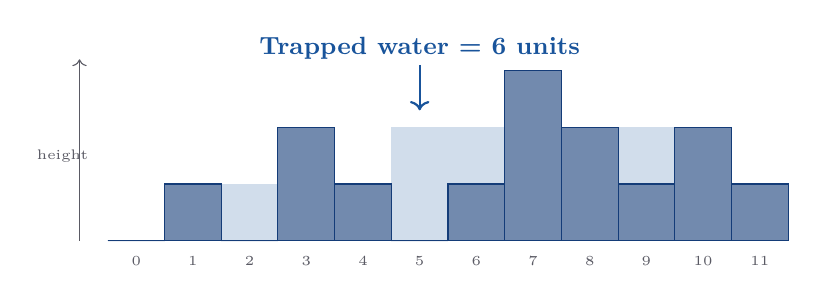
\begin{tikzpicture}[font=\small, scale=0.72]
  % Water fill (light blue rectangles behind bars)
  \fill[mybluelt!20] (2,0) rectangle (3,1);   % col 2, water up to 1
  \fill[mybluelt!20] (4,0) rectangle (5,1);   % col 4, water up to 1
  \fill[mybluelt!20] (5,0) rectangle (6,1);   % col 5
  \fill[mybluelt!20] (5,1) rectangle (6,2);
  \fill[mybluelt!20] (6,0) rectangle (7,1);   % col 6
  \fill[mybluelt!20] (6,1) rectangle (7,2);
  \fill[mybluelt!20] (9,0) rectangle (10,2);  % col 9
  \fill[mybluelt!20] (10,0) rectangle (11,1); % col 10

  % Bars
  \foreach \x/\h in {0/0,1/1,2/0,3/2,4/1,5/0,6/1,7/3,8/2,9/1,10/2,11/1}{
    \fill[myblue!60] (\x,0) rectangle (\x+1,\h);
    \draw[myblue] (\x,0) rectangle (\x+1,\h);
    \node[font=\tiny, text=mygray] at (\x+0.5,-0.35) {\x};
  }
  % Water label
  \node[text=mybluelt, font=\small\bfseries] at (5.5, 3.4) {Trapped water = 6 units};
  \draw[mybluelt, ->, thick] (5.5, 3.1) -- (5.5, 2.3);
  % Height label
  \node[text=mygray, font=\tiny] at (-0.8, 1.5) {height};
  \draw[mygray, ->] (-0.5, 0) -- (-0.5, 3.2);
\end{tikzpicture}
\end{center}

\textbf{Key Insight:} Water at index $i$ = $\min(\text{maxLeft}[i],\; \text{maxRight}[i]) - \text{height}[i]$.

The water level at any position is bounded by the \textit{shorter} of the tallest bars on its left and right. If that minimum exceeds the current bar height, water accumulates.

\subsection{Brute Force --- $O(n^2)$}

For each index, scan left and right to find the tallest bar on each side.

\begin{lstlisting}[caption={Trapping Rainwater --- Brute Force O(n$^2$)}]
public class TrappingRainwaterBrute {
    public static int trap(int[] height) {
        int n = height.length;
        int totalWater = 0;

        for (int i = 1; i < n - 1; i++) {
            // Find max height to the LEFT of i (including i)
            int maxLeft = 0;
            for (int j = 0; j <= i; j++) {
                maxLeft = Math.max(maxLeft, height[j]);
            }

            // Find max height to the RIGHT of i (including i)
            int maxRight = 0;
            for (int j = i; j < n; j++) {
                maxRight = Math.max(maxRight, height[j]);
            }

            // Water above this bar = min boundary - bar height
            totalWater += Math.min(maxLeft, maxRight) - height[i];
        }
        return totalWater;
    }
}
\end{lstlisting}

\begin{complexity}
Time: $O(n^2)$\quad Space: $O(1)$
\end{complexity}

\subsection{Prefix Array Approach --- $O(n)$ time $O(n)$ space}

Pre-compute \texttt{leftMax[]} and \texttt{rightMax[]} arrays, then calculate water in a single pass.

\begin{lstlisting}[caption={Trapping Rainwater --- Prefix Arrays O(n)}]
public class TrappingRainwaterPrefix {
    public static int trap(int[] height) {
        int n = height.length;
        if (n == 0) return 0;

        // leftMax[i]  = max height from index 0 to i  (inclusive)
        int[] leftMax  = new int[n];
        // rightMax[i] = max height from index i to n-1 (inclusive)
        int[] rightMax = new int[n];

        leftMax[0] = height[0];
        for (int i = 1; i < n; i++) {
            leftMax[i] = Math.max(leftMax[i - 1], height[i]);
        }

        rightMax[n - 1] = height[n - 1];
        for (int i = n - 2; i >= 0; i--) {
            rightMax[i] = Math.max(rightMax[i + 1], height[i]);
        }

        // Water at each index = min(leftMax, rightMax) - height[i]
        int totalWater = 0;
        for (int i = 0; i < n; i++) {
            totalWater += Math.min(leftMax[i], rightMax[i]) - height[i];
        }
        return totalWater;
    }

    public static void main(String[] args) {
        int[] h = {0,1,0,2,1,0,1,3,2,1,2,1};
        System.out.println(trap(h));  // 6
    }
}
\end{lstlisting}

\begin{dryrun}[height = \{0,1,0,2,1,0,1,3,2,1,2,1\}]
\begin{center}
\begin{tabular}{cccccc}
\toprule
\textbf{i} & \textbf{h[i]} & \textbf{leftMax} & \textbf{rightMax} & \textbf{min(L,R)} & \textbf{water}\\
\midrule
0 & 0 & 0 & 3 & 0 & 0\\
1 & 1 & 1 & 3 & 1 & 0\\
2 & 0 & 1 & 3 & 1 & \textbf{1}\\
3 & 2 & 2 & 3 & 2 & 0\\
4 & 1 & 2 & 3 & 2 & \textbf{1}\\
5 & 0 & 2 & 3 & 2 & \textbf{2}\\
6 & 1 & 2 & 3 & 2 & \textbf{1}\\
7 & 3 & 3 & 3 & 3 & 0\\
8 & 2 & 3 & 2 & 2 & 0\\
9 & 1 & 3 & 2 & 2 & \textbf{1}\\
10& 2 & 3 & 2 & 2 & 0\\
11& 1 & 3 & 1 & 1 & 0\\
\midrule
\multicolumn{5}{r}{\textbf{Total}} & \textbf{6}\\
\bottomrule
\end{tabular}
\end{center}
\end{dryrun}

\begin{complexity}
Time: $O(n)$ --- three linear passes\quad Space: $O(n)$ for two prefix arrays
\end{complexity}

\subsection{Two Pointer Approach --- $O(n)$ time $O(1)$ space (Optimal)}

Use two pointers moving inward. At any point, the side with the smaller max determines the water level --- no need to know the other side's max.

\begin{lstlisting}[caption={Trapping Rainwater --- Two Pointer O(n) time O(1) space}]
public class TrappingRainwaterTwoPointer {
    public static int trap(int[] height) {
        int left  = 0, right = height.length - 1;
        int leftMax = 0, rightMax = 0;
        int totalWater = 0;

        while (left < right) {
            if (height[left] <= height[right]) {
                // Left side is the bottleneck
                if (height[left] >= leftMax) {
                    leftMax = height[left];   // update left max
                } else {
                    totalWater += leftMax - height[left]; // water trapped
                }
                left++;
            } else {
                // Right side is the bottleneck
                if (height[right] >= rightMax) {
                    rightMax = height[right]; // update right max
                } else {
                    totalWater += rightMax - height[right]; // water trapped
                }
                right--;
            }
        }
        return totalWater;
    }

    public static void main(String[] args) {
        int[] h1 = {0,1,0,2,1,0,1,3,2,1,2,1};
        System.out.println(trap(h1));  // 6

        int[] h2 = {4,2,0,3,2,5};
        System.out.println(trap(h2));  // 9
    }
}
\end{lstlisting}

\begin{dryrun}[height = \{4, 2, 0, 3, 2, 5\}]
\begin{center}
\begin{tabular}{cccccccp{3cm}}
\toprule
\textbf{L} & \textbf{R} & \textbf{h[L]} & \textbf{h[R]} & \textbf{lMax} & \textbf{rMax} & \textbf{water} & \textbf{Action}\\
\midrule
0 & 5 & 4 & 5 & 0 & 0 & 0 & lMax=4, L++\\
1 & 5 & 2 & 5 & 4 & 0 & 0 & water+=2, L++\\
2 & 5 & 0 & 5 & 4 & 0 & 2 & water+=4, L++\\
3 & 5 & 3 & 5 & 4 & 0 & 6 & water+=1, L++\\
4 & 5 & 2 & 5 & 4 & 0 & 7 & water+=2, L++\\
5 & 5 & -- & -- & -- & -- & 9 & L$\not<$R: stop\\
\bottomrule
\end{tabular}
\end{center}
\textbf{Result: 9}
\end{dryrun}

\begin{complexity}
\begin{center}
\begin{tabular}{lll}
\toprule
\textbf{Approach} & \textbf{Time} & \textbf{Space}\\
\midrule
Brute Force              & $O(n^2)$  & $O(1)$\\
Prefix Arrays            & $O(n)$    & $O(n)$\\
Two Pointer (optimal)    & $O(n)$    & $O(1)$\\
\bottomrule
\end{tabular}
\end{center}
\end{complexity}

\begin{interviewcorner}
\begin{itemize}
  \item \textbf{Why two pointers work:} When \texttt{height[left] <= height[right]}, the water at \texttt{left} is determined by \texttt{leftMax} alone --- we already know \texttt{rightMax} $\geq$ \texttt{height[right]} $\geq$ \texttt{height[left]}, so the right boundary is never the bottleneck
  \item \textbf{Key formula:} water at index $i$ = $\max(0,\; \min(\text{leftMax}, \text{rightMax}) - \text{height}[i])$
  \item LeetCode 42 --- asked at Amazon, Google, Microsoft, Adobe
  \item Edge cases: empty array, single bar, monotonically increasing/decreasing (no water)
\end{itemize}
\end{interviewcorner}

%%------------------------------------------------------------
\section{Best Time to Buy and Sell Stock}
\index{Best Time to Buy and Sell Stock}
%%------------------------------------------------------------

\textbf{Problem:} Given an array \texttt{prices[]} where \texttt{prices[i]} is the price of a stock on day $i$, find the maximum profit you can achieve. You may complete at most \textbf{one} transaction (buy one, sell one). You must buy before you sell.

\textbf{Example:} \texttt{prices = [7, 1, 5, 3, 6, 4]} $\to$ answer = 5 (buy day 1 at \$1, sell day 4 at \$6)

\begin{center}
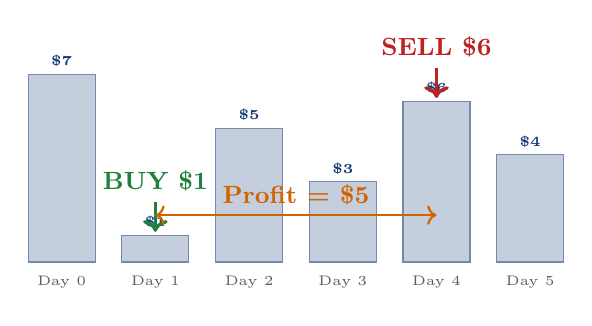
\begin{tikzpicture}[font=\small, scale=0.85]
  % Price bars
  \foreach \d/\p in {0/7, 1/1, 2/5, 3/3, 4/6, 5/4}{
    \fill[myblue!25] (\d*1.4, 0) rectangle (\d*1.4+1.0, \p*0.4);
    \draw[myblue!60] (\d*1.4, 0) rectangle (\d*1.4+1.0, \p*0.4);
    \node[font=\tiny, text=mygray] at (\d*1.4+0.5, -0.3) {Day \d};
    \node[font=\tiny\bfseries, text=myblue] at (\d*1.4+0.5, \p*0.4+0.2) {\$\p};
  }
  % Buy arrow
  \draw[mygreen, ->, very thick] (1.4+0.5, 1*0.4+0.5) node[above, text=mygreen, font=\small\bfseries]{BUY \$1} -- (1.4+0.5, 1*0.4+0.05);
  % Sell arrow
  \draw[myred, ->, very thick] (4*1.4+0.5, 6*0.4+0.5) node[above, text=myred, font=\small\bfseries]{SELL \$6} -- (4*1.4+0.5, 6*0.4+0.05);
  % Profit annotation
  \draw[myorange, <->, thick] (1.4+0.5, 0.7) -- (4*1.4+0.5, 0.7)
    node[midway, above, font=\small\bfseries, text=myorange]{Profit = \$5};
\end{tikzpicture}
\end{center}

\textbf{Key Insight:} Track the \textbf{minimum price seen so far} as you scan left to right. At each day, the best profit is \texttt{price[i] - minSoFar}. Keep the global maximum of all such profits.

\begin{lstlisting}[caption={Best Time to Buy and Sell Stock --- O(n) time O(1) space}]
public class BestTimeToBuySellStock {
    public static int maxProfit(int[] prices) {
        int minPrice  = Integer.MAX_VALUE;  // cheapest buying opportunity so far
        int maxProfit = 0;                  // best profit seen so far

        for (int i = 0; i < prices.length; i++) {

            if (prices[i] < minPrice) {
                minPrice = prices[i];       // found a cheaper day to buy
            } else if (prices[i] - minPrice > maxProfit) {
                maxProfit = prices[i] - minPrice; // found a better profit
            }
        }
        return maxProfit;
    }

    public static void main(String[] args) {
        int[] prices1 = {7, 1, 5, 3, 6, 4};
        System.out.println(maxProfit(prices1)); // 5  (buy@1 sell@6)

        int[] prices2 = {7, 6, 4, 3, 1};
        System.out.println(maxProfit(prices2)); // 0  (prices always fall, no profit)

        int[] prices3 = {1, 2};
        System.out.println(maxProfit(prices3)); // 1
    }
}
\end{lstlisting}

\begin{dryrun}[prices = \{7, 1, 5, 3, 6, 4\}]
\begin{center}
\begin{tabular}{ccccl}
\toprule
\textbf{i} & \textbf{prices[i]} & \textbf{minPrice} & \textbf{maxProfit} & \textbf{Note}\\
\midrule
0 & 7 & 7           & 0 & New min: 7\\
1 & 1 & \textbf{1}  & 0 & New min: 1\\
2 & 5 & 1           & \textbf{4} & Profit = 5-1 = 4\\
3 & 3 & 1           & 4 & Profit = 3-1 = 2, not better\\
4 & 6 & 1           & \textbf{5} & Profit = 6-1 = 5, new best!\\
5 & 4 & 1           & 5 & Profit = 4-1 = 3, not better\\
\bottomrule
\end{tabular}
\end{center}
\textbf{Result: maxProfit = 5}
\end{dryrun}

\begin{center}
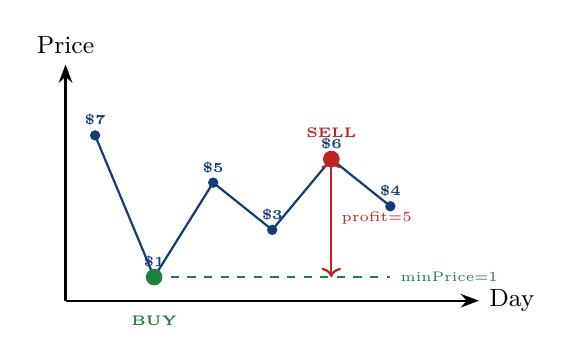
\begin{tikzpicture}[font=\small, scale=0.75]
  \draw[-{Stealth}, thick] (0,0) -- (7,0) node[right]{\small Day};
  \draw[-{Stealth}, thick] (0,0) -- (0,4) node[above]{\small Price};
  % Plot line
  \draw[myblue, thick] (0.5,2.8)--(1.5,0.4)--(2.5,2.0)--(3.5,1.2)--(4.5,2.4)--(5.5,1.6);
  \foreach \d/\p/\lbl in {0.5/2.8/7, 1.5/0.4/1, 2.5/2.0/5, 3.5/1.2/3, 4.5/2.4/6, 5.5/1.6/4}{
    \fill[myblue] (\d, \p) circle (2.5pt);
    \node[above, font=\tiny\bfseries, text=myblue] at (\d, \p) {\$\lbl};
  }
  % Min line
  \draw[mygreen, dashed, thick] (1.5,0.4) -- (5.5,0.4)
    node[right, text=mygreen, font=\tiny]{minPrice=1};
  % Best profit arrow
  \draw[myred, <->, thick] (4.5,0.4) -- (4.5,2.4)
    node[right, midway, text=myred, font=\tiny]{profit=5};
  % Dots at buy/sell
  \fill[mygreen] (1.5,0.4) circle (4pt);
  \fill[myred]   (4.5,2.4) circle (4pt);
  \node[below, text=mygreen, font=\tiny\bfseries] at (1.5,-0.1) {BUY};
  \node[above, text=myred,   font=\tiny\bfseries] at (4.5,2.6)  {SELL};
\end{tikzpicture}
\end{center}

\begin{complexity}
Time: $O(n)$ --- single pass\quad Space: $O(1)$ --- only two variables
\end{complexity}

\begin{interviewcorner}
\begin{itemize}
  \item \textbf{Why single pass works:} We always want to buy at the \textit{lowest price seen so far} and sell at the \textit{highest price after} that buy. Scanning left to right, \texttt{minPrice} gives the best buy opportunity up to the current day
  \item \textbf{What if prices always fall?} \texttt{maxProfit} stays 0 --- return 0, no transaction made
  \item \textbf{LeetCode 121} --- one of the most-asked problems at every major company
  \item \textbf{Follow-up: Multiple transactions (LeetCode 122)} --- you can buy and sell as many times as you want. Approach: greedily add every positive consecutive difference: \texttt{if (prices[i] > prices[i-1]) profit += prices[i] - prices[i-1]}
  \item \textbf{Follow-up: At most 2 transactions (LeetCode 123)} --- Dynamic programming with states
  \item Always check: is the sell day \textit{after} the buy day? (The single-pass approach guarantees this since \texttt{minPrice} is always from a previous or current day)
\end{itemize}
\end{interviewcorner}

\end{document}
